\documentclass[a4paper]{book}
\usepackage{a4wide}
\usepackage{makeidx}
\usepackage{fancyhdr}
\usepackage{graphicx}
\usepackage{multicol}
\usepackage{float}
\usepackage{textcomp}
\usepackage{alltt}
\usepackage{times}
\usepackage{ifpdf}
\ifpdf
\usepackage[pdftex,
            pagebackref=true,
            colorlinks=true,
            linkcolor=blue,
            unicode
           ]{hyperref}
\else
\usepackage[ps2pdf,
            pagebackref=true,
            colorlinks=true,
            linkcolor=blue,
            unicode
           ]{hyperref}
\usepackage{pspicture}
\fi
\usepackage[utf8]{inputenc}
\usepackage{doxygen}
\makeindex
\setcounter{tocdepth}{3}
\renewcommand{\footrulewidth}{0.4pt}
\begin{document}
\begin{titlepage}
\vspace*{7cm}
\begin{center}
{\Large AdaptiveMonteCarloonmultivariatebinaryspaces }\\
\vspace*{1cm}
{\large Generated by Doxygen 1.5.8}\\
\vspace*{0.5cm}
{\small Mon Oct 25 15:54:52 2010}\\
\end{center}
\end{titlepage}
\clearemptydoublepage
\pagenumbering{roman}
\tableofcontents
\clearemptydoublepage
\pagenumbering{arabic}
\chapter{Namespace Index}
\section{Namespace List}
Here is a list of all namespaces with brief descriptions:\begin{CompactList}
\item\contentsline{section}{\hyperlink{namespacebvnorm}{bvnorm} }{\pageref{namespacebvnorm}}{}
\item\contentsline{section}{\hyperlink{namespaceceopt}{ceopt} }{\pageref{namespaceceopt}}{}
\item\contentsline{section}{\hyperlink{namespacedefault}{default} }{\pageref{namespacedefault}}{}
\item\contentsline{section}{\hyperlink{namespaceeditcols}{editcols} }{\pageref{namespaceeditcols}}{}
\item\contentsline{section}{\hyperlink{namespaceeval}{eval} }{\pageref{namespaceeval}}{}
\item\contentsline{section}{\hyperlink{namespacegen}{gen} }{\pageref{namespacegen}}{}
\item\contentsline{section}{\hyperlink{namespacemcmc}{mcmc} }{\pageref{namespacemcmc}}{}
\item\contentsline{section}{\hyperlink{namespaceplotting}{plotting} }{\pageref{namespaceplotting}}{}
\item\contentsline{section}{\hyperlink{namespacesampling}{sampling} }{\pageref{namespacesampling}}{}
\item\contentsline{section}{\hyperlink{namespacesaopt}{saopt} }{\pageref{namespacesaopt}}{}
\item\contentsline{section}{\hyperlink{namespacesmc}{smc} }{\pageref{namespacesmc}}{}
\item\contentsline{section}{\hyperlink{namespacestarter}{starter} }{\pageref{namespacestarter}}{}
\item\contentsline{section}{\hyperlink{namespacetestfile}{testfile} }{\pageref{namespacetestfile}}{}
\end{CompactList}

\chapter{Class Index}
\section{Class Hierarchy}
This inheritance list is sorted roughly, but not completely, alphabetically:\begin{CompactList}
\item \contentsline{section}{gen::binary}{\pageref{classgen_1_1binary}}{}
\begin{CompactList}
\item \contentsline{section}{gen::binary\_\-ind}{\pageref{classgen_1_1binary__ind}}{}
\item \contentsline{section}{gen::binary\_\-log}{\pageref{classgen_1_1binary__log}}{}
\item \contentsline{section}{gen::binary\_\-mn}{\pageref{classgen_1_1binary__mn}}{}
\item \contentsline{section}{gen::binary\_\-post}{\pageref{classgen_1_1binary__post}}{}
\item \contentsline{section}{gen::binary\_\-post\_\-old}{\pageref{classgen_1_1binary__post__old}}{}
\end{CompactList}
\item \contentsline{section}{bvnorm::bvnorm\_\-gen}{\pageref{classbvnorm_1_1bvnorm__gen}}{}
\item \contentsline{section}{sampling::data}{\pageref{classsampling_1_1data}}{}
\item \contentsline{section}{mcmc::mcmc}{\pageref{classmcmc_1_1mcmc}}{}
\item \contentsline{section}{sampling::sampler}{\pageref{classsampling_1_1sampler}}{}
\item \contentsline{section}{smc::smc}{\pageref{classsmc_1_1smc}}{}
\end{CompactList}

\chapter{Class Index}
\section{Class List}
Here are the classes, structs, unions and interfaces with brief descriptions:\begin{CompactList}
\item\contentsline{section}{\hyperlink{classgen_1_1binary}{gen::binary} (The generator interface to be implemented by generators )}{\pageref{classgen_1_1binary}}{}
\item\contentsline{section}{\hyperlink{classgen_1_1binary__ind}{gen::binary\_\-ind} (Generates samples with independent components )}{\pageref{classgen_1_1binary__ind}}{}
\item\contentsline{section}{\hyperlink{classgen_1_1binary__log}{gen::binary\_\-log} }{\pageref{classgen_1_1binary__log}}{}
\item\contentsline{section}{\hyperlink{classgen_1_1binary__mn}{gen::binary\_\-mn} }{\pageref{classgen_1_1binary__mn}}{}
\item\contentsline{section}{\hyperlink{classgen_1_1binary__post}{gen::binary\_\-post} }{\pageref{classgen_1_1binary__post}}{}
\item\contentsline{section}{\hyperlink{classgen_1_1binary__post__old}{gen::binary\_\-post\_\-old} }{\pageref{classgen_1_1binary__post__old}}{}
\item\contentsline{section}{\hyperlink{classbvnorm_1_1bvnorm__gen}{bvnorm::bvnorm\_\-gen} }{\pageref{classbvnorm_1_1bvnorm__gen}}{}
\item\contentsline{section}{\hyperlink{classsampling_1_1data}{sampling::data} }{\pageref{classsampling_1_1data}}{}
\item\contentsline{section}{\hyperlink{classmcmc_1_1mcmc}{mcmc::mcmc} }{\pageref{classmcmc_1_1mcmc}}{}
\item\contentsline{section}{\hyperlink{classsampling_1_1sampler}{sampling::sampler} }{\pageref{classsampling_1_1sampler}}{}
\item\contentsline{section}{\hyperlink{classsmc_1_1smc}{smc::smc} (Sequential Monte Carlo class for model choice problems )}{\pageref{classsmc_1_1smc}}{}
\end{CompactList}

\chapter{File Index}
\section{File List}
Here is a list of all files with brief descriptions:\begin{CompactList}
\item\contentsline{section}{/mnt/eden/cschafer/Documents/smcdss/trunk/src/\hyperlink{bvnorm_8py}{bvnorm.py} }{\pageref{bvnorm_8py}}{}
\item\contentsline{section}{/mnt/eden/cschafer/Documents/smcdss/trunk/src/\hyperlink{ceopt_8py}{ceopt.py} }{\pageref{ceopt_8py}}{}
\item\contentsline{section}{/mnt/eden/cschafer/Documents/smcdss/trunk/src/\hyperlink{default_8py}{default.py} }{\pageref{default_8py}}{}
\item\contentsline{section}{/mnt/eden/cschafer/Documents/smcdss/trunk/src/\hyperlink{editcols_8py}{editcols.py} }{\pageref{editcols_8py}}{}
\item\contentsline{section}{/mnt/eden/cschafer/Documents/smcdss/trunk/src/\hyperlink{eval_8py}{eval.py} }{\pageref{eval_8py}}{}
\item\contentsline{section}{/mnt/eden/cschafer/Documents/smcdss/trunk/src/\hyperlink{gen_8py}{gen.py} }{\pageref{gen_8py}}{}
\item\contentsline{section}{/mnt/eden/cschafer/Documents/smcdss/trunk/src/\hyperlink{mcmc_8py}{mcmc.py} }{\pageref{mcmc_8py}}{}
\item\contentsline{section}{/mnt/eden/cschafer/Documents/smcdss/trunk/src/\hyperlink{plotting_8py}{plotting.py} }{\pageref{plotting_8py}}{}
\item\contentsline{section}{/mnt/eden/cschafer/Documents/smcdss/trunk/src/\hyperlink{sampling_8py}{sampling.py} }{\pageref{sampling_8py}}{}
\item\contentsline{section}{/mnt/eden/cschafer/Documents/smcdss/trunk/src/\hyperlink{saopt_8py}{saopt.py} }{\pageref{saopt_8py}}{}
\item\contentsline{section}{/mnt/eden/cschafer/Documents/smcdss/trunk/src/\hyperlink{smc_8py}{smc.py} }{\pageref{smc_8py}}{}
\item\contentsline{section}{/mnt/eden/cschafer/Documents/smcdss/trunk/src/\hyperlink{starter_8py}{starter.py} }{\pageref{starter_8py}}{}
\item\contentsline{section}{/mnt/eden/cschafer/Documents/smcdss/trunk/src/\hyperlink{testfile_8py}{testfile.py} }{\pageref{testfile_8py}}{}
\end{CompactList}

\chapter{Namespace Documentation}
\hypertarget{namespacebvnorm}{
\section{bvnorm Namespace Reference}
\label{namespacebvnorm}\index{bvnorm@{bvnorm}}
}
\subsection*{Classes}
\begin{CompactItemize}
\item 
class \hyperlink{classbvnorm_1_1bvnorm__gen}{bvnorm\_\-gen}
\end{CompactItemize}
\subsection*{Variables}
\begin{CompactItemize}
\item 
tuple \hyperlink{namespacebvnorm_ffd1e4833c9d3af70673f92d0e9bb471}{bvnorm} = \hyperlink{classbvnorm_1_1bvnorm__gen}{bvnorm\_\-gen}(name='\hyperlink{namespacebvnorm_ffd1e4833c9d3af70673f92d0e9bb471}{bvnorm}', longname='A bivariate normal', shapes='r', extradoc=\char`\"{}\char`\"{}\char`\"{}Bivariate normal distribution with correlation r.normal.pdf(x,y) = exp(-(x$\ast$x-2$\ast$r$\ast$x$\ast$y+y$\ast$y)/(2$\ast$(1-r$\ast$r))) / (2$\ast$pi$\ast$sqrt(1-r$\ast$r))\char`\"{}\char`\"{}\char`\"{})
\end{CompactItemize}


\subsection{Variable Documentation}
\hypertarget{namespacebvnorm_ffd1e4833c9d3af70673f92d0e9bb471}{
\index{bvnorm@{bvnorm}!bvnorm@{bvnorm}}
\index{bvnorm@{bvnorm}!bvnorm@{bvnorm}}
\subsubsection[{bvnorm}]{\setlength{\rightskip}{0pt plus 5cm}tuple {\bf bvnorm::bvnorm} = {\bf bvnorm\_\-gen}(name='{\bf bvnorm}', longname='A bivariate normal', shapes='r', extradoc=\char`\"{}\char`\"{}\char`\"{}Bivariate normal distribution with correlation r.normal.pdf(x,y) = exp(-(x$\ast$x-2$\ast$r$\ast$x$\ast$y+y$\ast$y)/(2$\ast$(1-r$\ast$r))) / (2$\ast$pi$\ast$sqrt(1-r$\ast$r))\char`\"{}\char`\"{}\char`\"{})}}
\label{namespacebvnorm_ffd1e4833c9d3af70673f92d0e9bb471}



\hypertarget{namespaceceopt}{
\section{ceopt Namespace Reference}
\label{namespaceceopt}\index{ceopt@{ceopt}}
}
\subsection*{Functions}
\begin{CompactItemize}
\item 
def \hyperlink{namespaceceopt_7c618a38f2a7288326b5cd95efc4be86}{ceopt}
\begin{CompactList}\small\item\em Run cross entropy optimization. \item\end{CompactList}\item 
def \hyperlink{namespaceceopt_7e223ba50a9bfff0599dd2ec8a823ca3}{cebrutesearch}
\begin{CompactList}\small\item\em Find the highest score and corresponding model by brute force search. \item\end{CompactList}\item 
def \hyperlink{namespaceceopt_59ffe1ffe93974a9623cac3917f0c409}{cetest}
\begin{CompactList}\small\item\em Run repeated tests of ce optimization. \item\end{CompactList}\item 
def \hyperlink{namespaceceopt_221be49549179d59d8c5bfe30706ca2c}{ceeval}
\begin{CompactList}\small\item\em Convert test runs into .eval-files and plots the respective histograms as .pdf-files. \item\end{CompactList}\item 
def \hyperlink{namespaceceopt_070fc29c5e852338e3352b09633c4fd3}{main}
\end{CompactItemize}
\subsection*{Variables}
\begin{CompactItemize}
\item 
string \hyperlink{namespaceceopt_909c15e21c1762433b80d29c7a095bc9}{TEST\_\-PATH} = '/home/cschafer/Documents/Python/workspace/\hyperlink{classsampling_1_1data}{data}/testruns'
\item 
string \hyperlink{namespaceceopt_cbf36072c5792daee6740a457808e012}{PDF\_\-PATH} = '/home/cschafer/Tex/amc\_\-on\_\-mbs/img/fragmaster'
\end{CompactItemize}


\subsection{Function Documentation}
\hypertarget{namespaceceopt_7e223ba50a9bfff0599dd2ec8a823ca3}{
\index{ceopt@{ceopt}!cebrutesearch@{cebrutesearch}}
\index{cebrutesearch@{cebrutesearch}!ceopt@{ceopt}}
\subsubsection[{cebrutesearch}]{\setlength{\rightskip}{0pt plus 5cm}def ceopt::cebrutesearch ( {\em gen}, \/   {\em targetDistr}, \/   {\em state\_\-max}, \/   {\em score\_\-max} = {\tt -inf})}}
\label{namespaceceopt_7e223ba50a9bfff0599dd2ec8a823ca3}


Find the highest score and corresponding model by brute force search. 

\hypertarget{namespaceceopt_221be49549179d59d8c5bfe30706ca2c}{
\index{ceopt@{ceopt}!ceeval@{ceeval}}
\index{ceeval@{ceeval}!ceopt@{ceopt}}
\subsubsection[{ceeval}]{\setlength{\rightskip}{0pt plus 5cm}def ceopt::ceeval ( {\em filename}, \/   {\em color} = {\tt False}, \/   {\em verbose} = {\tt False})}}
\label{namespaceceopt_221be49549179d59d8c5bfe30706ca2c}


Convert test runs into .eval-files and plots the respective histograms as .pdf-files. 

\hypertarget{namespaceceopt_7c618a38f2a7288326b5cd95efc4be86}{
\index{ceopt@{ceopt}!ceopt@{ceopt}}
\index{ceopt@{ceopt}!ceopt@{ceopt}}
\subsubsection[{ceopt}]{\setlength{\rightskip}{0pt plus 5cm}def ceopt::ceopt ( {\em targetDistr}, \/   {\em gens}, \/   {\em param}, \/   {\em nparticles}, \/   {\em plot}, \/   {\em verbose})}}
\label{namespaceceopt_7c618a38f2a7288326b5cd95efc4be86}


Run cross entropy optimization. 

\hypertarget{namespaceceopt_59ffe1ffe93974a9623cac3917f0c409}{
\index{ceopt@{ceopt}!cetest@{cetest}}
\index{cetest@{cetest}!ceopt@{ceopt}}
\subsubsection[{cetest}]{\setlength{\rightskip}{0pt plus 5cm}def ceopt::cetest ( {\em targetDistr}, \/   {\em gens}, \/   {\em param}, \/   {\em runs}, \/   {\em nparticles}, \/   {\em filestub}, \/   {\em test}, \/   {\em plot}, \/   {\em verbose})}}
\label{namespaceceopt_59ffe1ffe93974a9623cac3917f0c409}


Run repeated tests of ce optimization. 

\hypertarget{namespaceceopt_070fc29c5e852338e3352b09633c4fd3}{
\index{ceopt@{ceopt}!main@{main}}
\index{main@{main}!ceopt@{ceopt}}
\subsubsection[{main}]{\setlength{\rightskip}{0pt plus 5cm}def ceopt::main ()}}
\label{namespaceceopt_070fc29c5e852338e3352b09633c4fd3}




\subsection{Variable Documentation}
\hypertarget{namespaceceopt_cbf36072c5792daee6740a457808e012}{
\index{ceopt@{ceopt}!PDF\_\-PATH@{PDF\_\-PATH}}
\index{PDF\_\-PATH@{PDF\_\-PATH}!ceopt@{ceopt}}
\subsubsection[{PDF\_\-PATH}]{\setlength{\rightskip}{0pt plus 5cm}string {\bf ceopt::PDF\_\-PATH} = '/home/cschafer/Tex/amc\_\-on\_\-mbs/img/fragmaster'}}
\label{namespaceceopt_cbf36072c5792daee6740a457808e012}


\hypertarget{namespaceceopt_909c15e21c1762433b80d29c7a095bc9}{
\index{ceopt@{ceopt}!TEST\_\-PATH@{TEST\_\-PATH}}
\index{TEST\_\-PATH@{TEST\_\-PATH}!ceopt@{ceopt}}
\subsubsection[{TEST\_\-PATH}]{\setlength{\rightskip}{0pt plus 5cm}string {\bf ceopt::TEST\_\-PATH} = '/home/cschafer/Documents/Python/workspace/{\bf data}/testruns'}}
\label{namespaceceopt_909c15e21c1762433b80d29c7a095bc9}



\hypertarget{namespacedefault}{
\section{default Namespace Reference}
\label{namespacedefault}\index{default@{default}}
}
\subsection*{Variables}
\begin{CompactItemize}
\item 
string \hyperlink{namespacedefault_0c31828afc488101f96b519cb1cc97a4}{KERNEL} = 'MH'
\item 
int \hyperlink{namespacedefault_db3632d348cbdfb3166f68e74436e88a}{MAXTIME} = 30
\item 
string \hyperlink{namespacedefault_25dbe07c88b53f5e3d634a41030abc92}{THS\_\-ITER} = 'inf'
\item 
int \hyperlink{namespacedefault_e13d6e2cfb0c69b63bf1b94dc7b89f33}{NEIGHBORS} = 1
\item 
int \hyperlink{namespacedefault_a86f89a12973ba89585f8d3bf80e39bb}{NPARTICLES} = 20000
\item 
int \hyperlink{namespacedefault_f01f9265706877b864e148aa2497d491}{NBRIDGE} = 1
\item 
int \hyperlink{namespacedefault_2def7e326b1fcf05090331eb05eb87f0}{KAPPA} = 0
\item 
string \hyperlink{namespacedefault_011365b6827b95abcd94e942b9634033}{PROPOSAL} = 'logistic'
\item 
float \hyperlink{namespacedefault_b4c0f28797b1b7456f058a25d23f1b54}{FRACTION\_\-MEAN} = 0.02
\item 
float \hyperlink{namespacedefault_43dd32dbb17b845bfcdaf6c00b63388e}{FRACTION\_\-CORR} = 0.2
\item 
float \hyperlink{namespacedefault_f6f2749b29850745ee984eab37b6ff02}{SMOOTH\_\-MEAN} = 0.3
\item 
float \hyperlink{namespacedefault_76a017cb874d74e81d5094a72f1c52a6}{SMOOTH\_\-CORR} = 0.2
\item 
float \hyperlink{namespacedefault_6824ae496ae216b60d5f134a9bb0aaea}{THRESHOLD\_\-RANDOMNESS} = 0.02
\item 
int \hyperlink{namespacedefault_6ed59fbe2b196fcc3ae1a6b604276d6f}{MIN\_\-P} = 12
\item 
int \hyperlink{namespacedefault_d8fe4498e40472b3484b47a9b8f9b4f4}{NSTEPS} = 300000
\item 
\hyperlink{namespacedefault_9b628d43cf39c122618124e250f484d4}{TEST} = False
\item 
\hyperlink{namespacedefault_faa31f8e93aab4e3c4ac7150c07a2163}{VERBOSE} = False
\item 
int \hyperlink{namespacedefault_5a47bc24cc2e81c2b486201e0150ed2d}{RUNS} = 200
\item 
string \hyperlink{namespacedefault_16c08c1aa9ed63675d727816602bd477}{SCORETYPE} = 'hb'
\item 
string \hyperlink{namespacedefault_050715858d86503e16fb8c76ba80f8ef}{DATASET} = 'boston'
\item 
string \hyperlink{namespacedefault_5f4c31e5e7cfc29df6f2858a2823e01e}{DATA\_\-PATH} = ''
\item 
string \hyperlink{namespacedefault_67f5df46d57b595458bd2b48834fa686}{OUTFILE\_\-PATH} = ''
\item 
float \hyperlink{namespacedefault_97d9d8ec55531a1738ba8e112b028503}{BOXDATA} = 0.8
\item 
\hyperlink{namespacedefault_6c7b3398123a66516eb33bdd5be92f72}{FRAGMASTER} = False
\item 
\hyperlink{namespacedefault_75efb1111f068d4ec2410c969f8e8163}{TITLES} = False
\item 
\hyperlink{namespacedefault_e15b6feffdfa11718d2f69bed850b8e5}{COLOR} = False
\item 
int \hyperlink{namespacedefault_afe0a3920f5df428cdac98ff509ecb64}{NUMBER} = 1
\item 
string \hyperlink{namespacedefault_a394b7f75e7cdba5f60003c6db292474}{EVAL\_\-PATH} = ''
\item 
string \hyperlink{namespacedefault_8d9fb97268090be4e6cec6c944f44a56}{FRAGMASTER\_\-PATH} = ''
\item 
list \hyperlink{namespacedefault_d933462cfca0c3f8181f44fc9f57060d}{OUTER\_\-MARGIN} = \mbox{[}40, 4, 5, 4\mbox{]}
\item 
list \hyperlink{namespacedefault_fb792579817a22922ee3388b3ab96b27}{INNER\_\-MARGIN} = \mbox{[}0, 0, 0, 0\mbox{]}
\item 
string \hyperlink{namespacedefault_9b4e126bc71dd911f1f777eb99e81064}{FONT\_\-FAMILY} = 'serif'
\item 
int \hyperlink{namespacedefault_38fe4c2b86af6bcf5c5a4b568a55b865}{TITLE\_\-LINE} = 1
\end{CompactItemize}


\subsection{Variable Documentation}
\hypertarget{namespacedefault_97d9d8ec55531a1738ba8e112b028503}{
\index{default@{default}!BOXDATA@{BOXDATA}}
\index{BOXDATA@{BOXDATA}!default@{default}}
\subsubsection[{BOXDATA}]{\setlength{\rightskip}{0pt plus 5cm}float {\bf default::BOXDATA} = 0.8}}
\label{namespacedefault_97d9d8ec55531a1738ba8e112b028503}


\hypertarget{namespacedefault_e15b6feffdfa11718d2f69bed850b8e5}{
\index{default@{default}!COLOR@{COLOR}}
\index{COLOR@{COLOR}!default@{default}}
\subsubsection[{COLOR}]{\setlength{\rightskip}{0pt plus 5cm}{\bf default::COLOR} = False}}
\label{namespacedefault_e15b6feffdfa11718d2f69bed850b8e5}


\hypertarget{namespacedefault_5f4c31e5e7cfc29df6f2858a2823e01e}{
\index{default@{default}!DATA\_\-PATH@{DATA\_\-PATH}}
\index{DATA\_\-PATH@{DATA\_\-PATH}!default@{default}}
\subsubsection[{DATA\_\-PATH}]{\setlength{\rightskip}{0pt plus 5cm}string {\bf default::DATA\_\-PATH} = ''}}
\label{namespacedefault_5f4c31e5e7cfc29df6f2858a2823e01e}


\hypertarget{namespacedefault_050715858d86503e16fb8c76ba80f8ef}{
\index{default@{default}!DATASET@{DATASET}}
\index{DATASET@{DATASET}!default@{default}}
\subsubsection[{DATASET}]{\setlength{\rightskip}{0pt plus 5cm}string {\bf default::DATASET} = 'boston'}}
\label{namespacedefault_050715858d86503e16fb8c76ba80f8ef}


\hypertarget{namespacedefault_a394b7f75e7cdba5f60003c6db292474}{
\index{default@{default}!EVAL\_\-PATH@{EVAL\_\-PATH}}
\index{EVAL\_\-PATH@{EVAL\_\-PATH}!default@{default}}
\subsubsection[{EVAL\_\-PATH}]{\setlength{\rightskip}{0pt plus 5cm}string {\bf default::EVAL\_\-PATH} = ''}}
\label{namespacedefault_a394b7f75e7cdba5f60003c6db292474}


\hypertarget{namespacedefault_9b4e126bc71dd911f1f777eb99e81064}{
\index{default@{default}!FONT\_\-FAMILY@{FONT\_\-FAMILY}}
\index{FONT\_\-FAMILY@{FONT\_\-FAMILY}!default@{default}}
\subsubsection[{FONT\_\-FAMILY}]{\setlength{\rightskip}{0pt plus 5cm}string {\bf default::FONT\_\-FAMILY} = 'serif'}}
\label{namespacedefault_9b4e126bc71dd911f1f777eb99e81064}


\hypertarget{namespacedefault_43dd32dbb17b845bfcdaf6c00b63388e}{
\index{default@{default}!FRACTION\_\-CORR@{FRACTION\_\-CORR}}
\index{FRACTION\_\-CORR@{FRACTION\_\-CORR}!default@{default}}
\subsubsection[{FRACTION\_\-CORR}]{\setlength{\rightskip}{0pt plus 5cm}float {\bf default::FRACTION\_\-CORR} = 0.2}}
\label{namespacedefault_43dd32dbb17b845bfcdaf6c00b63388e}


\hypertarget{namespacedefault_b4c0f28797b1b7456f058a25d23f1b54}{
\index{default@{default}!FRACTION\_\-MEAN@{FRACTION\_\-MEAN}}
\index{FRACTION\_\-MEAN@{FRACTION\_\-MEAN}!default@{default}}
\subsubsection[{FRACTION\_\-MEAN}]{\setlength{\rightskip}{0pt plus 5cm}float {\bf default::FRACTION\_\-MEAN} = 0.02}}
\label{namespacedefault_b4c0f28797b1b7456f058a25d23f1b54}


\hypertarget{namespacedefault_6c7b3398123a66516eb33bdd5be92f72}{
\index{default@{default}!FRAGMASTER@{FRAGMASTER}}
\index{FRAGMASTER@{FRAGMASTER}!default@{default}}
\subsubsection[{FRAGMASTER}]{\setlength{\rightskip}{0pt plus 5cm}{\bf default::FRAGMASTER} = False}}
\label{namespacedefault_6c7b3398123a66516eb33bdd5be92f72}


\hypertarget{namespacedefault_8d9fb97268090be4e6cec6c944f44a56}{
\index{default@{default}!FRAGMASTER\_\-PATH@{FRAGMASTER\_\-PATH}}
\index{FRAGMASTER\_\-PATH@{FRAGMASTER\_\-PATH}!default@{default}}
\subsubsection[{FRAGMASTER\_\-PATH}]{\setlength{\rightskip}{0pt plus 5cm}string {\bf default::FRAGMASTER\_\-PATH} = ''}}
\label{namespacedefault_8d9fb97268090be4e6cec6c944f44a56}


\hypertarget{namespacedefault_fb792579817a22922ee3388b3ab96b27}{
\index{default@{default}!INNER\_\-MARGIN@{INNER\_\-MARGIN}}
\index{INNER\_\-MARGIN@{INNER\_\-MARGIN}!default@{default}}
\subsubsection[{INNER\_\-MARGIN}]{\setlength{\rightskip}{0pt plus 5cm}list {\bf default::INNER\_\-MARGIN} = \mbox{[}0, 0, 0, 0\mbox{]}}}
\label{namespacedefault_fb792579817a22922ee3388b3ab96b27}


\hypertarget{namespacedefault_2def7e326b1fcf05090331eb05eb87f0}{
\index{default@{default}!KAPPA@{KAPPA}}
\index{KAPPA@{KAPPA}!default@{default}}
\subsubsection[{KAPPA}]{\setlength{\rightskip}{0pt plus 5cm}int {\bf default::KAPPA} = 0}}
\label{namespacedefault_2def7e326b1fcf05090331eb05eb87f0}


\hypertarget{namespacedefault_0c31828afc488101f96b519cb1cc97a4}{
\index{default@{default}!KERNEL@{KERNEL}}
\index{KERNEL@{KERNEL}!default@{default}}
\subsubsection[{KERNEL}]{\setlength{\rightskip}{0pt plus 5cm}string {\bf default::KERNEL} = 'MH'}}
\label{namespacedefault_0c31828afc488101f96b519cb1cc97a4}


\hypertarget{namespacedefault_db3632d348cbdfb3166f68e74436e88a}{
\index{default@{default}!MAXTIME@{MAXTIME}}
\index{MAXTIME@{MAXTIME}!default@{default}}
\subsubsection[{MAXTIME}]{\setlength{\rightskip}{0pt plus 5cm}int {\bf default::MAXTIME} = 30}}
\label{namespacedefault_db3632d348cbdfb3166f68e74436e88a}


\hypertarget{namespacedefault_6ed59fbe2b196fcc3ae1a6b604276d6f}{
\index{default@{default}!MIN\_\-P@{MIN\_\-P}}
\index{MIN\_\-P@{MIN\_\-P}!default@{default}}
\subsubsection[{MIN\_\-P}]{\setlength{\rightskip}{0pt plus 5cm}int {\bf default::MIN\_\-P} = 12}}
\label{namespacedefault_6ed59fbe2b196fcc3ae1a6b604276d6f}


\hypertarget{namespacedefault_f01f9265706877b864e148aa2497d491}{
\index{default@{default}!NBRIDGE@{NBRIDGE}}
\index{NBRIDGE@{NBRIDGE}!default@{default}}
\subsubsection[{NBRIDGE}]{\setlength{\rightskip}{0pt plus 5cm}int {\bf default::NBRIDGE} = 1}}
\label{namespacedefault_f01f9265706877b864e148aa2497d491}


\hypertarget{namespacedefault_e13d6e2cfb0c69b63bf1b94dc7b89f33}{
\index{default@{default}!NEIGHBORS@{NEIGHBORS}}
\index{NEIGHBORS@{NEIGHBORS}!default@{default}}
\subsubsection[{NEIGHBORS}]{\setlength{\rightskip}{0pt plus 5cm}int {\bf default::NEIGHBORS} = 1}}
\label{namespacedefault_e13d6e2cfb0c69b63bf1b94dc7b89f33}


\hypertarget{namespacedefault_a86f89a12973ba89585f8d3bf80e39bb}{
\index{default@{default}!NPARTICLES@{NPARTICLES}}
\index{NPARTICLES@{NPARTICLES}!default@{default}}
\subsubsection[{NPARTICLES}]{\setlength{\rightskip}{0pt plus 5cm}int {\bf default::NPARTICLES} = 20000}}
\label{namespacedefault_a86f89a12973ba89585f8d3bf80e39bb}


\hypertarget{namespacedefault_d8fe4498e40472b3484b47a9b8f9b4f4}{
\index{default@{default}!NSTEPS@{NSTEPS}}
\index{NSTEPS@{NSTEPS}!default@{default}}
\subsubsection[{NSTEPS}]{\setlength{\rightskip}{0pt plus 5cm}int {\bf default::NSTEPS} = 300000}}
\label{namespacedefault_d8fe4498e40472b3484b47a9b8f9b4f4}


\hypertarget{namespacedefault_afe0a3920f5df428cdac98ff509ecb64}{
\index{default@{default}!NUMBER@{NUMBER}}
\index{NUMBER@{NUMBER}!default@{default}}
\subsubsection[{NUMBER}]{\setlength{\rightskip}{0pt plus 5cm}int {\bf default::NUMBER} = 1}}
\label{namespacedefault_afe0a3920f5df428cdac98ff509ecb64}


\hypertarget{namespacedefault_d933462cfca0c3f8181f44fc9f57060d}{
\index{default@{default}!OUTER\_\-MARGIN@{OUTER\_\-MARGIN}}
\index{OUTER\_\-MARGIN@{OUTER\_\-MARGIN}!default@{default}}
\subsubsection[{OUTER\_\-MARGIN}]{\setlength{\rightskip}{0pt plus 5cm}list {\bf default::OUTER\_\-MARGIN} = \mbox{[}40, 4, 5, 4\mbox{]}}}
\label{namespacedefault_d933462cfca0c3f8181f44fc9f57060d}


\hypertarget{namespacedefault_67f5df46d57b595458bd2b48834fa686}{
\index{default@{default}!OUTFILE\_\-PATH@{OUTFILE\_\-PATH}}
\index{OUTFILE\_\-PATH@{OUTFILE\_\-PATH}!default@{default}}
\subsubsection[{OUTFILE\_\-PATH}]{\setlength{\rightskip}{0pt plus 5cm}string {\bf default::OUTFILE\_\-PATH} = ''}}
\label{namespacedefault_67f5df46d57b595458bd2b48834fa686}


\hypertarget{namespacedefault_011365b6827b95abcd94e942b9634033}{
\index{default@{default}!PROPOSAL@{PROPOSAL}}
\index{PROPOSAL@{PROPOSAL}!default@{default}}
\subsubsection[{PROPOSAL}]{\setlength{\rightskip}{0pt plus 5cm}string {\bf default::PROPOSAL} = 'logistic'}}
\label{namespacedefault_011365b6827b95abcd94e942b9634033}


\hypertarget{namespacedefault_5a47bc24cc2e81c2b486201e0150ed2d}{
\index{default@{default}!RUNS@{RUNS}}
\index{RUNS@{RUNS}!default@{default}}
\subsubsection[{RUNS}]{\setlength{\rightskip}{0pt plus 5cm}int {\bf default::RUNS} = 200}}
\label{namespacedefault_5a47bc24cc2e81c2b486201e0150ed2d}


\hypertarget{namespacedefault_16c08c1aa9ed63675d727816602bd477}{
\index{default@{default}!SCORETYPE@{SCORETYPE}}
\index{SCORETYPE@{SCORETYPE}!default@{default}}
\subsubsection[{SCORETYPE}]{\setlength{\rightskip}{0pt plus 5cm}string {\bf default::SCORETYPE} = 'hb'}}
\label{namespacedefault_16c08c1aa9ed63675d727816602bd477}


\hypertarget{namespacedefault_76a017cb874d74e81d5094a72f1c52a6}{
\index{default@{default}!SMOOTH\_\-CORR@{SMOOTH\_\-CORR}}
\index{SMOOTH\_\-CORR@{SMOOTH\_\-CORR}!default@{default}}
\subsubsection[{SMOOTH\_\-CORR}]{\setlength{\rightskip}{0pt plus 5cm}float {\bf default::SMOOTH\_\-CORR} = 0.2}}
\label{namespacedefault_76a017cb874d74e81d5094a72f1c52a6}


\hypertarget{namespacedefault_f6f2749b29850745ee984eab37b6ff02}{
\index{default@{default}!SMOOTH\_\-MEAN@{SMOOTH\_\-MEAN}}
\index{SMOOTH\_\-MEAN@{SMOOTH\_\-MEAN}!default@{default}}
\subsubsection[{SMOOTH\_\-MEAN}]{\setlength{\rightskip}{0pt plus 5cm}float {\bf default::SMOOTH\_\-MEAN} = 0.3}}
\label{namespacedefault_f6f2749b29850745ee984eab37b6ff02}


\hypertarget{namespacedefault_9b628d43cf39c122618124e250f484d4}{
\index{default@{default}!TEST@{TEST}}
\index{TEST@{TEST}!default@{default}}
\subsubsection[{TEST}]{\setlength{\rightskip}{0pt plus 5cm}{\bf default::TEST} = False}}
\label{namespacedefault_9b628d43cf39c122618124e250f484d4}


\hypertarget{namespacedefault_6824ae496ae216b60d5f134a9bb0aaea}{
\index{default@{default}!THRESHOLD\_\-RANDOMNESS@{THRESHOLD\_\-RANDOMNESS}}
\index{THRESHOLD\_\-RANDOMNESS@{THRESHOLD\_\-RANDOMNESS}!default@{default}}
\subsubsection[{THRESHOLD\_\-RANDOMNESS}]{\setlength{\rightskip}{0pt plus 5cm}float {\bf default::THRESHOLD\_\-RANDOMNESS} = 0.02}}
\label{namespacedefault_6824ae496ae216b60d5f134a9bb0aaea}


\hypertarget{namespacedefault_25dbe07c88b53f5e3d634a41030abc92}{
\index{default@{default}!THS\_\-ITER@{THS\_\-ITER}}
\index{THS\_\-ITER@{THS\_\-ITER}!default@{default}}
\subsubsection[{THS\_\-ITER}]{\setlength{\rightskip}{0pt plus 5cm}string {\bf default::THS\_\-ITER} = 'inf'}}
\label{namespacedefault_25dbe07c88b53f5e3d634a41030abc92}


\hypertarget{namespacedefault_38fe4c2b86af6bcf5c5a4b568a55b865}{
\index{default@{default}!TITLE\_\-LINE@{TITLE\_\-LINE}}
\index{TITLE\_\-LINE@{TITLE\_\-LINE}!default@{default}}
\subsubsection[{TITLE\_\-LINE}]{\setlength{\rightskip}{0pt plus 5cm}int {\bf default::TITLE\_\-LINE} = 1}}
\label{namespacedefault_38fe4c2b86af6bcf5c5a4b568a55b865}


\hypertarget{namespacedefault_75efb1111f068d4ec2410c969f8e8163}{
\index{default@{default}!TITLES@{TITLES}}
\index{TITLES@{TITLES}!default@{default}}
\subsubsection[{TITLES}]{\setlength{\rightskip}{0pt plus 5cm}{\bf default::TITLES} = False}}
\label{namespacedefault_75efb1111f068d4ec2410c969f8e8163}


\hypertarget{namespacedefault_faa31f8e93aab4e3c4ac7150c07a2163}{
\index{default@{default}!VERBOSE@{VERBOSE}}
\index{VERBOSE@{VERBOSE}!default@{default}}
\subsubsection[{VERBOSE}]{\setlength{\rightskip}{0pt plus 5cm}{\bf default::VERBOSE} = False}}
\label{namespacedefault_faa31f8e93aab4e3c4ac7150c07a2163}



\hypertarget{namespaceeditcols}{
\section{editcols Namespace Reference}
\label{namespaceeditcols}\index{editcols@{editcols}}
}
\subsection*{Functions}
\begin{CompactItemize}
\item 
def \hyperlink{namespaceeditcols_a92bfbedd2a1f59a4741b1bb2b4b1a38}{editcols}
\item 
def \hyperlink{namespaceeditcols_41465a54c2a568b6abad72ffbb139917}{main}
\end{CompactItemize}


\subsection{Function Documentation}
\hypertarget{namespaceeditcols_a92bfbedd2a1f59a4741b1bb2b4b1a38}{
\index{editcols@{editcols}!editcols@{editcols}}
\index{editcols@{editcols}!editcols@{editcols}}
\subsubsection[{editcols}]{\setlength{\rightskip}{0pt plus 5cm}def editcols::editcols ( {\em args})}}
\label{namespaceeditcols_a92bfbedd2a1f59a4741b1bb2b4b1a38}


\hypertarget{namespaceeditcols_41465a54c2a568b6abad72ffbb139917}{
\index{editcols@{editcols}!main@{main}}
\index{main@{main}!editcols@{editcols}}
\subsubsection[{main}]{\setlength{\rightskip}{0pt plus 5cm}def editcols::main ()}}
\label{namespaceeditcols_41465a54c2a568b6abad72ffbb139917}



\hypertarget{namespaceeval}{
\section{eval Namespace Reference}
\label{namespaceeval}\index{eval@{eval}}
}
\subsection*{Functions}
\begin{CompactItemize}
\item 
def \hyperlink{namespaceeval_2852fcd5af5e95c3f5548a3a51b0c52e}{maketitle}
\item 
def \hyperlink{namespaceeval_c26f3aa5011d54adf5e4c1fbe53a0f54}{evalest}
\begin{CompactList}\small\item\em Make pdf-boxplots from testfiles. \item\end{CompactList}\item 
def \hyperlink{namespaceeval_0dcd0d97820f287e38e356cdf3da3a0c}{evalopt}
\item 
def \hyperlink{namespaceeval_e3b126f2e6d2aa6c1ed96ecf02d91e8d}{main}
\begin{CompactList}\small\item\em Parse command line options to smctest. \item\end{CompactList}\end{CompactItemize}
\subsection*{Variables}
\begin{CompactItemize}
\item 
string \hyperlink{namespaceeval_257985d7d7884932360c75335c8e5052}{TEST\_\-PATH} = '/home/cschafer/Documents/Python/workspace/\hyperlink{classsampling_1_1data}{data}/testruns'
\item 
string \hyperlink{namespaceeval_0f22d22751fdd8f5b825e7484476fe1d}{PDF\_\-PATH} = '/home/cschafer/Tex'
\end{CompactItemize}


\subsection{Function Documentation}
\hypertarget{namespaceeval_c26f3aa5011d54adf5e4c1fbe53a0f54}{
\index{eval@{eval}!evalest@{evalest}}
\index{evalest@{evalest}!eval@{eval}}
\subsubsection[{evalest}]{\setlength{\rightskip}{0pt plus 5cm}def eval::evalest ( {\em filestubs} = {\tt \mbox{[}'$\ast$'\mbox{]}}, \/   {\em boxdata} = {\tt 0.8}, \/   {\em titles} = {\tt False}, \/   {\em color} = {\tt False})}}
\label{namespaceeval_c26f3aa5011d54adf5e4c1fbe53a0f54}


Make pdf-boxplots from testfiles. 

\begin{Desc}
\item[Parameters:]
\begin{description}
\item[{\em file}]Name of the \hyperlink{namespacetestfile}{testfile} to be processed. \item[{\em boxdata}]Percentage of data to be included in the core of the boxplot. \end{description}
\end{Desc}
\hypertarget{namespaceeval_0dcd0d97820f287e38e356cdf3da3a0c}{
\index{eval@{eval}!evalopt@{evalopt}}
\index{evalopt@{evalopt}!eval@{eval}}
\subsubsection[{evalopt}]{\setlength{\rightskip}{0pt plus 5cm}def eval::evalopt ( {\em filestubs} = {\tt \mbox{[}'$\ast$'\mbox{]}}, \/   {\em number} = {\tt None}, \/   {\em boxdata} = {\tt 0.8}, \/   {\em titles} = {\tt False}, \/   {\em color} = {\tt False})}}
\label{namespaceeval_0dcd0d97820f287e38e356cdf3da3a0c}


\hypertarget{namespaceeval_e3b126f2e6d2aa6c1ed96ecf02d91e8d}{
\index{eval@{eval}!main@{main}}
\index{main@{main}!eval@{eval}}
\subsubsection[{main}]{\setlength{\rightskip}{0pt plus 5cm}def eval::main ()}}
\label{namespaceeval_e3b126f2e6d2aa6c1ed96ecf02d91e8d}


Parse command line options to smctest. 

Type evalt --help for help. \hypertarget{namespaceeval_2852fcd5af5e95c3f5548a3a51b0c52e}{
\index{eval@{eval}!maketitle@{maketitle}}
\index{maketitle@{maketitle}!eval@{eval}}
\subsubsection[{maketitle}]{\setlength{\rightskip}{0pt plus 5cm}def eval::maketitle ( {\em file})}}
\label{namespaceeval_2852fcd5af5e95c3f5548a3a51b0c52e}




\subsection{Variable Documentation}
\hypertarget{namespaceeval_0f22d22751fdd8f5b825e7484476fe1d}{
\index{eval@{eval}!PDF\_\-PATH@{PDF\_\-PATH}}
\index{PDF\_\-PATH@{PDF\_\-PATH}!eval@{eval}}
\subsubsection[{PDF\_\-PATH}]{\setlength{\rightskip}{0pt plus 5cm}string {\bf eval::PDF\_\-PATH} = '/home/cschafer/Tex'}}
\label{namespaceeval_0f22d22751fdd8f5b825e7484476fe1d}


\hypertarget{namespaceeval_257985d7d7884932360c75335c8e5052}{
\index{eval@{eval}!TEST\_\-PATH@{TEST\_\-PATH}}
\index{TEST\_\-PATH@{TEST\_\-PATH}!eval@{eval}}
\subsubsection[{TEST\_\-PATH}]{\setlength{\rightskip}{0pt plus 5cm}string {\bf eval::TEST\_\-PATH} = '/home/cschafer/Documents/Python/workspace/{\bf data}/testruns'}}
\label{namespaceeval_257985d7d7884932360c75335c8e5052}



\hypertarget{namespacegen}{
\section{gen Namespace Reference}
\label{namespacegen}\index{gen@{gen}}
}
\subsection*{Classes}
\begin{CompactItemize}
\item 
class \hyperlink{classgen_1_1binary}{binary}
\begin{CompactList}\small\item\em The generator interface to be implemented by generators. \item\end{CompactList}\item 
class \hyperlink{classgen_1_1binary__ind}{binary\_\-ind}
\begin{CompactList}\small\item\em Generates samples with independent components. \item\end{CompactList}\item 
class \hyperlink{classgen_1_1binary__mn}{binary\_\-mn}
\item 
class \hyperlink{classgen_1_1binary__log}{binary\_\-log}
\item 
class \hyperlink{classgen_1_1binary__post__old}{binary\_\-post\_\-old}
\item 
class \hyperlink{classgen_1_1binary__post}{binary\_\-post}
\end{CompactItemize}
\subsection*{Functions}
\begin{CompactItemize}
\item 
def \hyperlink{namespacegen_6b7ade8b5daf3fe3773bbd616e9e2b42}{bin2dec}
\begin{CompactList}\small\item\em Converts a boolean array into an integer. \item\end{CompactList}\item 
def \hyperlink{namespacegen_21553f88e5b189da2003268cfabb215f}{bin2str}
\begin{CompactList}\small\item\em Converts a boolean array into a \hyperlink{classgen_1_1binary}{binary} string. \item\end{CompactList}\item 
def \hyperlink{namespacegen_804c568d405e9b3b8234ca18666fd0e3}{dec2bin}
\begin{CompactList}\small\item\em Converts an integer into a boolean array containing its \hyperlink{classgen_1_1binary}{binary} representation. \item\end{CompactList}\item 
def \hyperlink{namespacegen_287d3a33d4580585adcc84c10c39082a}{crosscols}
\begin{CompactList}\small\item\em Returns an array of all pairs between firstcol and lastcol. \item\end{CompactList}\end{CompactItemize}
\subsection*{Variables}
\begin{CompactItemize}
\item 
\hyperlink{namespacegen_448acbda618185ee4482080762551d0c}{WEAVE} = True
\item 
int \hyperlink{namespacegen_283eb6a0f532506a7be95ca53d71ef06}{DECIMALS} = 10
\begin{CompactList}\small\item\em precision for breakin \item\end{CompactList}\item 
int \hyperlink{namespacegen_257a6a4ead271854ce0abaee1e27ce1d}{LOOPS} = 25
\begin{CompactList}\small\item\em maximum number of loops \item\end{CompactList}\item 
int \hyperlink{namespacegen_d75234477e080aeb312e8cb2813d5ba6}{MAX\_\-FEASIBLE} = 12
\begin{CompactList}\small\item\em maximum size feasible for exhaustive exploration \item\end{CompactList}\item 
string \hyperlink{namespacegen_cd9fd05ba9face577992611e21fd84ca}{PATH} = \char`\"{}/home/cschafer/Eden/Documents/Python/workspace\char`\"{}
\item 
\hyperlink{namespacegen_362c029b7eeb5fb3c67104ac5a218849}{hasrpy} = True
\end{CompactItemize}


\subsection{Function Documentation}
\hypertarget{namespacegen_6b7ade8b5daf3fe3773bbd616e9e2b42}{
\index{gen@{gen}!bin2dec@{bin2dec}}
\index{bin2dec@{bin2dec}!gen@{gen}}
\subsubsection[{bin2dec}]{\setlength{\rightskip}{0pt plus 5cm}def gen::bin2dec ( {\em b})}}
\label{namespacegen_6b7ade8b5daf3fe3773bbd616e9e2b42}


Converts a boolean array into an integer. 

\hypertarget{namespacegen_21553f88e5b189da2003268cfabb215f}{
\index{gen@{gen}!bin2str@{bin2str}}
\index{bin2str@{bin2str}!gen@{gen}}
\subsubsection[{bin2str}]{\setlength{\rightskip}{0pt plus 5cm}def gen::bin2str ( {\em b})}}
\label{namespacegen_21553f88e5b189da2003268cfabb215f}


Converts a boolean array into a \hyperlink{classgen_1_1binary}{binary} string. 

\hypertarget{namespacegen_287d3a33d4580585adcc84c10c39082a}{
\index{gen@{gen}!crosscols@{crosscols}}
\index{crosscols@{crosscols}!gen@{gen}}
\subsubsection[{crosscols}]{\setlength{\rightskip}{0pt plus 5cm}def gen::crosscols ( {\em firstcol}, \/   {\em lastcol})}}
\label{namespacegen_287d3a33d4580585adcc84c10c39082a}


Returns an array of all pairs between firstcol and lastcol. 

\hypertarget{namespacegen_804c568d405e9b3b8234ca18666fd0e3}{
\index{gen@{gen}!dec2bin@{dec2bin}}
\index{dec2bin@{dec2bin}!gen@{gen}}
\subsubsection[{dec2bin}]{\setlength{\rightskip}{0pt plus 5cm}def gen::dec2bin ( {\em n}, \/   {\em dim} = {\tt 0})}}
\label{namespacegen_804c568d405e9b3b8234ca18666fd0e3}


Converts an integer into a boolean array containing its \hyperlink{classgen_1_1binary}{binary} representation. 



\subsection{Variable Documentation}
\hypertarget{namespacegen_283eb6a0f532506a7be95ca53d71ef06}{
\index{gen@{gen}!DECIMALS@{DECIMALS}}
\index{DECIMALS@{DECIMALS}!gen@{gen}}
\subsubsection[{DECIMALS}]{\setlength{\rightskip}{0pt plus 5cm}int {\bf gen::DECIMALS} = 10}}
\label{namespacegen_283eb6a0f532506a7be95ca53d71ef06}


precision for breakin 

\hypertarget{namespacegen_362c029b7eeb5fb3c67104ac5a218849}{
\index{gen@{gen}!hasrpy@{hasrpy}}
\index{hasrpy@{hasrpy}!gen@{gen}}
\subsubsection[{hasrpy}]{\setlength{\rightskip}{0pt plus 5cm}{\bf gen::hasrpy} = True}}
\label{namespacegen_362c029b7eeb5fb3c67104ac5a218849}


\hypertarget{namespacegen_257a6a4ead271854ce0abaee1e27ce1d}{
\index{gen@{gen}!LOOPS@{LOOPS}}
\index{LOOPS@{LOOPS}!gen@{gen}}
\subsubsection[{LOOPS}]{\setlength{\rightskip}{0pt plus 5cm}int {\bf gen::LOOPS} = 25}}
\label{namespacegen_257a6a4ead271854ce0abaee1e27ce1d}


maximum number of loops 

\hypertarget{namespacegen_d75234477e080aeb312e8cb2813d5ba6}{
\index{gen@{gen}!MAX\_\-FEASIBLE@{MAX\_\-FEASIBLE}}
\index{MAX\_\-FEASIBLE@{MAX\_\-FEASIBLE}!gen@{gen}}
\subsubsection[{MAX\_\-FEASIBLE}]{\setlength{\rightskip}{0pt plus 5cm}int {\bf gen::MAX\_\-FEASIBLE} = 12}}
\label{namespacegen_d75234477e080aeb312e8cb2813d5ba6}


maximum size feasible for exhaustive exploration 

\hypertarget{namespacegen_cd9fd05ba9face577992611e21fd84ca}{
\index{gen@{gen}!PATH@{PATH}}
\index{PATH@{PATH}!gen@{gen}}
\subsubsection[{PATH}]{\setlength{\rightskip}{0pt plus 5cm}string {\bf gen::PATH} = \char`\"{}/home/cschafer/Eden/Documents/Python/workspace\char`\"{}}}
\label{namespacegen_cd9fd05ba9face577992611e21fd84ca}


\hypertarget{namespacegen_448acbda618185ee4482080762551d0c}{
\index{gen@{gen}!WEAVE@{WEAVE}}
\index{WEAVE@{WEAVE}!gen@{gen}}
\subsubsection[{WEAVE}]{\setlength{\rightskip}{0pt plus 5cm}{\bf gen::WEAVE} = True}}
\label{namespacegen_448acbda618185ee4482080762551d0c}



\hypertarget{namespacemcmc}{
\section{mcmc Namespace Reference}
\label{namespacemcmc}\index{mcmc@{mcmc}}
}
\subsection*{Classes}
\begin{CompactItemize}
\item 
class \hyperlink{classmcmc_1_1mcmc}{mcmc}
\end{CompactItemize}
\subsection*{Functions}
\begin{CompactItemize}
\item 
def \hyperlink{namespacemcmc_60fb0f78f00fa057c4f90a4a7ed2f111}{mcmctest}
\begin{CompactList}\small\item\em Run repeated tests of bridge \hyperlink{namespacesmc}{smc}. \item\end{CompactList}\item 
def \hyperlink{namespacemcmc_4ad3e26158616bd6ddc216215bd5198c}{mcmceval}
\begin{CompactList}\small\item\em Plot test run quantiles as .pdf-files. \item\end{CompactList}\item 
def \hyperlink{namespacemcmc_3320bffb49a11dc6dc758ebe59506f51}{main}
\end{CompactItemize}
\subsection*{Variables}
\begin{CompactItemize}
\item 
string \hyperlink{namespacemcmc_ed142f91127f59debb6ed1904b67d983}{PATH} = '/home/cschafer/Documents/Python/workspace/\hyperlink{classsampling_1_1data}{data}'
\end{CompactItemize}


\subsection{Function Documentation}
\hypertarget{namespacemcmc_3320bffb49a11dc6dc758ebe59506f51}{
\index{mcmc@{mcmc}!main@{main}}
\index{main@{main}!mcmc@{mcmc}}
\subsubsection[{main}]{\setlength{\rightskip}{0pt plus 5cm}def mcmc::main ()}}
\label{namespacemcmc_3320bffb49a11dc6dc758ebe59506f51}


\hypertarget{namespacemcmc_4ad3e26158616bd6ddc216215bd5198c}{
\index{mcmc@{mcmc}!mcmceval@{mcmceval}}
\index{mcmceval@{mcmceval}!mcmc@{mcmc}}
\subsubsection[{mcmceval}]{\setlength{\rightskip}{0pt plus 5cm}def mcmc::mcmceval ( {\em filename} = {\tt PATH~+~'/testruns'}, \/   {\em boxdata} = {\tt 0.8})}}
\label{namespacemcmc_4ad3e26158616bd6ddc216215bd5198c}


Plot test run quantiles as .pdf-files. 

\hypertarget{namespacemcmc_60fb0f78f00fa057c4f90a4a7ed2f111}{
\index{mcmc@{mcmc}!mcmctest@{mcmctest}}
\index{mcmctest@{mcmctest}!mcmc@{mcmc}}
\subsubsection[{mcmctest}]{\setlength{\rightskip}{0pt plus 5cm}def mcmc::mcmctest ( {\em targetDistr}, \/   {\em filestub}, \/   {\em runs}, \/   {\em kernel}, \/   {\em test}, \/   {\em plot}, \/   {\em verbose}, \/   {\em maxtime} = {\tt inf}, \/   {\em ths\_\-iter} = {\tt inf})}}
\label{namespacemcmc_60fb0f78f00fa057c4f90a4a7ed2f111}


Run repeated tests of bridge \hyperlink{namespacesmc}{smc}. 



\subsection{Variable Documentation}
\hypertarget{namespacemcmc_ed142f91127f59debb6ed1904b67d983}{
\index{mcmc@{mcmc}!PATH@{PATH}}
\index{PATH@{PATH}!mcmc@{mcmc}}
\subsubsection[{PATH}]{\setlength{\rightskip}{0pt plus 5cm}string {\bf mcmc::PATH} = '/home/cschafer/Documents/Python/workspace/{\bf data}'}}
\label{namespacemcmc_ed142f91127f59debb6ed1904b67d983}



\hypertarget{namespaceplotting}{
\section{plotting Namespace Reference}
\label{namespaceplotting}\index{plotting@{plotting}}
}
\subsection*{Functions}
\begin{CompactItemize}
\item 
def \hyperlink{namespaceplotting_b505da9b5173fdd94b5900e8a9017160}{plotSteps}
\begin{CompactList}\small\item\em Plots the marginal probabilites and correlation matrix of each step during ce optimization. \item\end{CompactList}\item 
def \hyperlink{namespaceplotting_40bdd65430f0e2b3e2fbe73977a45976}{plot4}
\begin{CompactList}\small\item\em Generates perfect samples from the posterior and initializes an independent, multinormal and log regression generator to plot their respective histograms. \item\end{CompactList}\end{CompactItemize}
\subsection*{Variables}
\begin{CompactItemize}
\item 
string \hyperlink{namespaceplotting_9422d71ff1b0ed3d54e826072cbc5df6}{PATH} = '/home/cschafer/Documents/Python/workspace/\hyperlink{classsampling_1_1data}{data}'
\end{CompactItemize}


\subsection{Function Documentation}
\hypertarget{namespaceplotting_40bdd65430f0e2b3e2fbe73977a45976}{
\index{plotting@{plotting}!plot4@{plot4}}
\index{plot4@{plot4}!plotting@{plotting}}
\subsubsection[{plot4}]{\setlength{\rightskip}{0pt plus 5cm}def plotting::plot4 ( {\em post}, \/   {\em m} = {\tt 1500}, \/   {\em n} = {\tt 2000}, \/   {\em verbose} = {\tt True})}}
\label{namespaceplotting_40bdd65430f0e2b3e2fbe73977a45976}


Generates perfect samples from the posterior and initializes an independent, multinormal and log regression generator to plot their respective histograms. 

\hypertarget{namespaceplotting_b505da9b5173fdd94b5900e8a9017160}{
\index{plotting@{plotting}!plotSteps@{plotSteps}}
\index{plotSteps@{plotSteps}!plotting@{plotting}}
\subsubsection[{plotSteps}]{\setlength{\rightskip}{0pt plus 5cm}def plotting::plotSteps ( {\em left}, \/   {\em right}, \/   {\em step}, \/   {\em plotdir} = {\tt \char`\"{}pdf/step\char`\"{}}, \/   {\em diff} = {\tt False})}}
\label{namespaceplotting_b505da9b5173fdd94b5900e8a9017160}


Plots the marginal probabilites and correlation matrix of each step during ce optimization. 



\subsection{Variable Documentation}
\hypertarget{namespaceplotting_9422d71ff1b0ed3d54e826072cbc5df6}{
\index{plotting@{plotting}!PATH@{PATH}}
\index{PATH@{PATH}!plotting@{plotting}}
\subsubsection[{PATH}]{\setlength{\rightskip}{0pt plus 5cm}string {\bf plotting::PATH} = '/home/cschafer/Documents/Python/workspace/{\bf data}'}}
\label{namespaceplotting_9422d71ff1b0ed3d54e826072cbc5df6}



\hypertarget{namespacesampling}{
\section{sampling Namespace Reference}
\label{namespacesampling}\index{sampling@{sampling}}
}
\subsection*{Classes}
\begin{CompactItemize}
\item 
class \hyperlink{classsampling_1_1data}{data}
\item 
class \hyperlink{classsampling_1_1sampler}{sampler}
\end{CompactItemize}

\hypertarget{namespacesaopt}{
\section{saopt Namespace Reference}
\label{namespacesaopt}\index{saopt@{saopt}}
}
\subsection*{Functions}
\begin{CompactItemize}
\item 
def \hyperlink{namespacesaopt_27363a0082deed7804d30ebdf145cd0a}{saopt}
\begin{CompactList}\small\item\em Run simulated annealing optimization. \item\end{CompactList}\item 
def \hyperlink{namespacesaopt_515091c950b58a3cc0c8e785fc3f802a}{satest}
\begin{CompactList}\small\item\em Run repeated tests of sa optimization. \item\end{CompactList}\item 
def \hyperlink{namespacesaopt_cc9749cdc655806017ef69dc2654c483}{main}
\end{CompactItemize}
\subsection*{Variables}
\begin{CompactItemize}
\item 
string \hyperlink{namespacesaopt_4077ce3616d15b802bafa0748162883e}{TEST\_\-PATH} = '/home/cschafer/Documents/Python/workspace/\hyperlink{classsampling_1_1data}{data}/testruns'
\end{CompactItemize}


\subsection{Function Documentation}
\hypertarget{namespacesaopt_cc9749cdc655806017ef69dc2654c483}{
\index{saopt@{saopt}!main@{main}}
\index{main@{main}!saopt@{saopt}}
\subsubsection[{main}]{\setlength{\rightskip}{0pt plus 5cm}def saopt::main ()}}
\label{namespacesaopt_cc9749cdc655806017ef69dc2654c483}


\hypertarget{namespacesaopt_27363a0082deed7804d30ebdf145cd0a}{
\index{saopt@{saopt}!saopt@{saopt}}
\index{saopt@{saopt}!saopt@{saopt}}
\subsubsection[{saopt}]{\setlength{\rightskip}{0pt plus 5cm}def saopt::saopt ( {\em targetDistr}, \/   {\em n}, \/   {\em verbose})}}
\label{namespacesaopt_27363a0082deed7804d30ebdf145cd0a}


Run simulated annealing optimization. 

\hypertarget{namespacesaopt_515091c950b58a3cc0c8e785fc3f802a}{
\index{saopt@{saopt}!satest@{satest}}
\index{satest@{satest}!saopt@{saopt}}
\subsubsection[{satest}]{\setlength{\rightskip}{0pt plus 5cm}def saopt::satest ( {\em targetDistr}, \/   {\em runs}, \/   {\em n}, \/   {\em filestub}, \/   {\em test}, \/   {\em verbose})}}
\label{namespacesaopt_515091c950b58a3cc0c8e785fc3f802a}


Run repeated tests of sa optimization. 



\subsection{Variable Documentation}
\hypertarget{namespacesaopt_4077ce3616d15b802bafa0748162883e}{
\index{saopt@{saopt}!TEST\_\-PATH@{TEST\_\-PATH}}
\index{TEST\_\-PATH@{TEST\_\-PATH}!saopt@{saopt}}
\subsubsection[{TEST\_\-PATH}]{\setlength{\rightskip}{0pt plus 5cm}string {\bf saopt::TEST\_\-PATH} = '/home/cschafer/Documents/Python/workspace/{\bf data}/testruns'}}
\label{namespacesaopt_4077ce3616d15b802bafa0748162883e}



\hypertarget{namespacesmc}{
\section{smc Namespace Reference}
\label{namespacesmc}\index{smc@{smc}}
}
\subsection*{Classes}
\begin{CompactItemize}
\item 
class \hyperlink{classsmc_1_1smc}{smc}
\begin{CompactList}\small\item\em Sequential Monte Carlo class for model choice problems. \item\end{CompactList}\end{CompactItemize}
\subsection*{Functions}
\begin{CompactItemize}
\item 
def \hyperlink{namespacesmc_90ae893d3420c53ca98ea6d16a27ebf6}{smctest}
\begin{CompactList}\small\item\em Run repeated tests of bridge \hyperlink{namespacesmc}{smc}. \item\end{CompactList}\item 
def \hyperlink{namespacesmc_e7960431b019652bb6041acbe319314a}{smceval}
\begin{CompactList}\small\item\em Make pdf-boxplots from testfiles. \item\end{CompactList}\item 
def \hyperlink{namespacesmc_060a055567983af558dd15bda3d5a7be}{main}
\begin{CompactList}\small\item\em Parse command line options to smctest. \item\end{CompactList}\end{CompactItemize}
\subsection*{Variables}
\begin{CompactItemize}
\item 
\hyperlink{namespacesmc_fa23f48b546729c612828f8c434748d3}{WEAVE} = False
\begin{CompactList}\small\item\em True, if scipy.weave is available. \item\end{CompactList}\item 
string \hyperlink{namespacesmc_e5f7d905ee9ecc1f072955328a069bba}{PATH} = '/home/cschafer/Documents/Python/workspace/\hyperlink{classsampling_1_1data}{data}'
\begin{CompactList}\small\item\em Absolute path to the data directory. \item\end{CompactList}\end{CompactItemize}


\subsection{Function Documentation}
\hypertarget{namespacesmc_060a055567983af558dd15bda3d5a7be}{
\index{smc@{smc}!main@{main}}
\index{main@{main}!smc@{smc}}
\subsubsection[{main}]{\setlength{\rightskip}{0pt plus 5cm}def smc::main ()}}
\label{namespacesmc_060a055567983af558dd15bda3d5a7be}


Parse command line options to smctest. 

Type \hyperlink{namespacesmc}{smc} --help for help. \hypertarget{namespacesmc_e7960431b019652bb6041acbe319314a}{
\index{smc@{smc}!smceval@{smceval}}
\index{smceval@{smceval}!smc@{smc}}
\subsubsection[{smceval}]{\setlength{\rightskip}{0pt plus 5cm}def smc::smceval ( {\em filestubs} = {\tt '$\ast$'}, \/   {\em boxdata} = {\tt 0.8}, \/   {\em fragmaster} = {\tt False})}}
\label{namespacesmc_e7960431b019652bb6041acbe319314a}


Make pdf-boxplots from testfiles. 

\begin{Desc}
\item[Parameters:]
\begin{description}
\item[{\em filename}]Name of the \hyperlink{namespacetestfile}{testfile} to be processed. \item[{\em boxdata}]Percentage of data to be included in the core of the boxplot. \end{description}
\end{Desc}
\hypertarget{namespacesmc_90ae893d3420c53ca98ea6d16a27ebf6}{
\index{smc@{smc}!smctest@{smctest}}
\index{smctest@{smctest}!smc@{smc}}
\subsubsection[{smctest}]{\setlength{\rightskip}{0pt plus 5cm}def smc::smctest ( {\em targetDistr}, \/   {\em filestub}, \/   {\em runs}, \/   {\em nbridge}, \/   {\em nparticles}, \/   {\em kappa}, \/   {\em test}, \/   {\em plot}, \/   {\em verbose})}}
\label{namespacesmc_90ae893d3420c53ca98ea6d16a27ebf6}


Run repeated tests of bridge \hyperlink{namespacesmc}{smc}. 

\begin{Desc}
\item[Parameters:]
\begin{description}
\item[{\em targetDistr}]The target distribution. \item[{\em filestub}]Name of the test-file without numbering. \item[{\em runs}]Number of testruns to perform. \item[{\em nbridge}]Number of bridge steps between the prior and the target. \item[{\em nparticles}]Number of particles. \item[{\em kappa}]Prior smoothing parameter: 0 $<$= kappa $<$= 1. \item[{\em test}]True, if no \hyperlink{namespacetestfile}{testfile} is desired. \item[{\em plot}]True, if the steps are to be plotted. \item[{\em verbose}]True, if reports to standard are desired. \end{description}
\end{Desc}


\subsection{Variable Documentation}
\hypertarget{namespacesmc_e5f7d905ee9ecc1f072955328a069bba}{
\index{smc@{smc}!PATH@{PATH}}
\index{PATH@{PATH}!smc@{smc}}
\subsubsection[{PATH}]{\setlength{\rightskip}{0pt plus 5cm}string {\bf smc::PATH} = '/home/cschafer/Documents/Python/workspace/{\bf data}'}}
\label{namespacesmc_e5f7d905ee9ecc1f072955328a069bba}


Absolute path to the data directory. 

\hypertarget{namespacesmc_fa23f48b546729c612828f8c434748d3}{
\index{smc@{smc}!WEAVE@{WEAVE}}
\index{WEAVE@{WEAVE}!smc@{smc}}
\subsubsection[{WEAVE}]{\setlength{\rightskip}{0pt plus 5cm}{\bf smc::WEAVE} = False}}
\label{namespacesmc_fa23f48b546729c612828f8c434748d3}


True, if scipy.weave is available. 


\hypertarget{namespacestarter}{
\section{starter Namespace Reference}
\label{namespacestarter}\index{starter@{starter}}
}
\subsection*{Functions}
\begin{CompactItemize}
\item 
def \hyperlink{namespacestarter_e0a0cc7ba8875c428361e4e9b1fdbe37}{starter}
\item 
def \hyperlink{namespacestarter_69dcc5f42ff248c07a8db4132c72ccc2}{main}
\end{CompactItemize}


\subsection{Function Documentation}
\hypertarget{namespacestarter_69dcc5f42ff248c07a8db4132c72ccc2}{
\index{starter@{starter}!main@{main}}
\index{main@{main}!starter@{starter}}
\subsubsection[{main}]{\setlength{\rightskip}{0pt plus 5cm}def starter::main ()}}
\label{namespacestarter_69dcc5f42ff248c07a8db4132c72ccc2}


\hypertarget{namespacestarter_e0a0cc7ba8875c428361e4e9b1fdbe37}{
\index{starter@{starter}!starter@{starter}}
\index{starter@{starter}!starter@{starter}}
\subsubsection[{starter}]{\setlength{\rightskip}{0pt plus 5cm}def starter::starter ( {\em args})}}
\label{namespacestarter_e0a0cc7ba8875c428361e4e9b1fdbe37}



\hypertarget{namespacetestfile}{
\section{testfile Namespace Reference}
\label{namespacetestfile}\index{testfile@{testfile}}
}
\subsection*{Functions}
\begin{CompactItemize}
\item 
def \hyperlink{namespacetestfile_99113854298691c9eeb8a8898644a974}{dec2bin}
\item 
def \hyperlink{namespacetestfile_4072711694fcae0f9109bc45c7bb49ba}{randomModel}
\item 
def \hyperlink{namespacetestfile_3d8b61f805030ee5a2344dcd3c3c99c2}{loglinear}
\item 
def \hyperlink{namespacetestfile_9ca7719f709048d58857d39899d701de}{computeMU}
\item 
def \hyperlink{namespacetestfile_67f6cac6991933db387292d093863552}{marginal\_\-loglinear}
\item 
def \hyperlink{namespacetestfile_4d944ca85cf8ac83c850faaf02a61361}{computeMOMENTS}
\item 
def \hyperlink{namespacetestfile_bfa1bb5dd9c351ed90706ff1c941046d}{printMOMENTS}
\end{CompactItemize}
\subsection*{Variables}
\begin{CompactItemize}
\item 
int \hyperlink{namespacetestfile_91df5af6cb9c0d7b55401a5f33b65bd5}{DIM} = 6
\item 
tuple \hyperlink{namespacetestfile_1651280ab7e62f5b47d4526ce503f08e}{ALPHA}
\item 
int \hyperlink{namespacetestfile_a00aea5cbc11b484cdd7edce5d1c1807}{MU} = 0
\end{CompactItemize}


\subsection{Function Documentation}
\hypertarget{namespacetestfile_4d944ca85cf8ac83c850faaf02a61361}{
\index{testfile@{testfile}!computeMOMENTS@{computeMOMENTS}}
\index{computeMOMENTS@{computeMOMENTS}!testfile@{testfile}}
\subsubsection[{computeMOMENTS}]{\setlength{\rightskip}{0pt plus 5cm}def testfile::computeMOMENTS ( {\em dim})}}
\label{namespacetestfile_4d944ca85cf8ac83c850faaf02a61361}


\hypertarget{namespacetestfile_9ca7719f709048d58857d39899d701de}{
\index{testfile@{testfile}!computeMU@{computeMU}}
\index{computeMU@{computeMU}!testfile@{testfile}}
\subsubsection[{computeMU}]{\setlength{\rightskip}{0pt plus 5cm}def testfile::computeMU ()}}
\label{namespacetestfile_9ca7719f709048d58857d39899d701de}


\hypertarget{namespacetestfile_99113854298691c9eeb8a8898644a974}{
\index{testfile@{testfile}!dec2bin@{dec2bin}}
\index{dec2bin@{dec2bin}!testfile@{testfile}}
\subsubsection[{dec2bin}]{\setlength{\rightskip}{0pt plus 5cm}def testfile::dec2bin ( {\em n}, \/   {\em dim} = {\tt 0})}}
\label{namespacetestfile_99113854298691c9eeb8a8898644a974}


\hypertarget{namespacetestfile_3d8b61f805030ee5a2344dcd3c3c99c2}{
\index{testfile@{testfile}!loglinear@{loglinear}}
\index{loglinear@{loglinear}!testfile@{testfile}}
\subsubsection[{loglinear}]{\setlength{\rightskip}{0pt plus 5cm}def testfile::loglinear ( {\em b})}}
\label{namespacetestfile_3d8b61f805030ee5a2344dcd3c3c99c2}


\hypertarget{namespacetestfile_67f6cac6991933db387292d093863552}{
\index{testfile@{testfile}!marginal\_\-loglinear@{marginal\_\-loglinear}}
\index{marginal\_\-loglinear@{marginal\_\-loglinear}!testfile@{testfile}}
\subsubsection[{marginal\_\-loglinear}]{\setlength{\rightskip}{0pt plus 5cm}def testfile::marginal\_\-loglinear ( {\em b})}}
\label{namespacetestfile_67f6cac6991933db387292d093863552}


\hypertarget{namespacetestfile_bfa1bb5dd9c351ed90706ff1c941046d}{
\index{testfile@{testfile}!printMOMENTS@{printMOMENTS}}
\index{printMOMENTS@{printMOMENTS}!testfile@{testfile}}
\subsubsection[{printMOMENTS}]{\setlength{\rightskip}{0pt plus 5cm}def testfile::printMOMENTS ( {\em dim})}}
\label{namespacetestfile_bfa1bb5dd9c351ed90706ff1c941046d}


\hypertarget{namespacetestfile_4072711694fcae0f9109bc45c7bb49ba}{
\index{testfile@{testfile}!randomModel@{randomModel}}
\index{randomModel@{randomModel}!testfile@{testfile}}
\subsubsection[{randomModel}]{\setlength{\rightskip}{0pt plus 5cm}def testfile::randomModel ( {\em dim})}}
\label{namespacetestfile_4072711694fcae0f9109bc45c7bb49ba}




\subsection{Variable Documentation}
\hypertarget{namespacetestfile_1651280ab7e62f5b47d4526ce503f08e}{
\index{testfile@{testfile}!ALPHA@{ALPHA}}
\index{ALPHA@{ALPHA}!testfile@{testfile}}
\subsubsection[{ALPHA}]{\setlength{\rightskip}{0pt plus 5cm}tuple {\bf testfile::ALPHA}}}
\label{namespacetestfile_1651280ab7e62f5b47d4526ce503f08e}


\textbf{Initial value:}

\begin{Code}\begin{verbatim}array(\
[-0.97882863, 0.61502143, 0.03769291, 0.23966928, 0.31955478, 0.02240849,\
  0.61502143,-0.58855963,-0.08270103,-0.29593133,-0.13480816,-0.17921533,\
 -0.03769291, 0.08270103, 0.17368193, 0.08290546,-0.04733021, 0.15170509,\
  0.23966928,-0.29593133,-0.08290546,-0.49613294, 0.26298699,-0.32414626,\
  0.31955478,-0.13480816, 0.04733021,-0.26298699,-0.35536491,-0.01111059,\
 -0.02240849, 0.17921533, 0.15170509, 0.32414626, 0.01111059, 0.35519851])
\end{verbatim}
\end{Code}
\hypertarget{namespacetestfile_91df5af6cb9c0d7b55401a5f33b65bd5}{
\index{testfile@{testfile}!DIM@{DIM}}
\index{DIM@{DIM}!testfile@{testfile}}
\subsubsection[{DIM}]{\setlength{\rightskip}{0pt plus 5cm}int {\bf testfile::DIM} = 6}}
\label{namespacetestfile_91df5af6cb9c0d7b55401a5f33b65bd5}


\hypertarget{namespacetestfile_a00aea5cbc11b484cdd7edce5d1c1807}{
\index{testfile@{testfile}!MU@{MU}}
\index{MU@{MU}!testfile@{testfile}}
\subsubsection[{MU}]{\setlength{\rightskip}{0pt plus 5cm}tuple {\bf testfile::MU} = 0}}
\label{namespacetestfile_a00aea5cbc11b484cdd7edce5d1c1807}



\chapter{Class Documentation}
\hypertarget{classgen_1_1binary}{
\section{gen::binary Class Reference}
\label{classgen_1_1binary}\index{gen::binary@{gen::binary}}
}
The generator interface to be implemented by generators.  


Inheritance diagram for gen::binary::\begin{figure}[H]
\begin{center}
\leavevmode
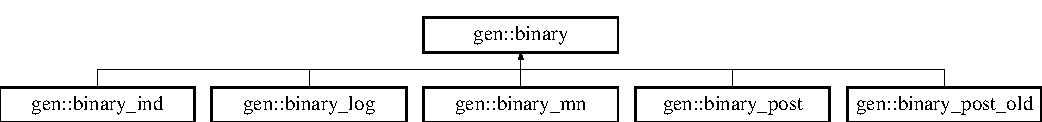
\includegraphics[height=1.63504cm]{classgen_1_1binary}
\end{center}
\end{figure}
\subsection*{Public Member Functions}
\begin{CompactItemize}
\item 
def \hyperlink{classgen_1_1binary_705669a0b9879ed4c0f3b1d7ebac7163}{\_\-\_\-init\_\-\_\-}
\item 
def \hyperlink{classgen_1_1binary_8fd0271b697cfd36fc72a5e3dadbd908}{reset}
\item 
def \hyperlink{classgen_1_1binary_2a0d104e1d99419fa3c5e7bf5db96e9e}{pmf}
\item 
def \hyperlink{classgen_1_1binary_0377b3ffdd44806d72453d0b8ead1758}{lpmf}
\item 
def \hyperlink{classgen_1_1binary_02fc0fab1e701e3f02f564eb7577e0d2}{rvs}
\begin{CompactList}\small\item\em Generate a random variable. \item\end{CompactList}\item 
def \hyperlink{classgen_1_1binary_07a67826e434eeb49aaef326d2e41805}{plot}
\begin{CompactList}\small\item\em Plots the probability distribution function of the generator (if possible). \item\end{CompactList}\item 
def \hyperlink{classgen_1_1binary_9cf0ff8452df83ccbae5ba1e56136645}{hist}
\begin{CompactList}\small\item\em Plots a histogram of the empirical distribution obtained by \hyperlink{namespacesampling}{sampling} from the generator. \item\end{CompactList}\end{CompactItemize}
\subsection*{Public Attributes}
\begin{CompactItemize}
\item 
\hyperlink{classgen_1_1binary_ca500be68fab85fb9606fcb4c5be8f64}{nozero}
\item 
\hyperlink{classgen_1_1binary_37e0504e82a2e1117ed23ff2d8617274}{dim}
\item 
\hyperlink{classgen_1_1binary_ca3be8a3fef7eeebd95bdcd5b5a82a5b}{min\_\-p}
\item 
\hyperlink{classgen_1_1binary_aec6d5ee9de0b2a4ddf0a9fa1ced25ae}{adjusted}
\item 
\hyperlink{classgen_1_1binary_156a3b3004ee18dc4472dbbb22e58441}{data}
\item 
\hyperlink{classgen_1_1binary_d525c9bbdde203e71bfbd20ab8a3b87b}{fraction\_\-mean}
\item 
\hyperlink{classgen_1_1binary_1e3b4573f717d0c9a1c0e04c02f2fd00}{fraction\_\-corr}
\item 
\hyperlink{classgen_1_1binary_37a0b8a17b6838931cc090b0bd420113}{smooth\_\-mean}
\item 
\hyperlink{classgen_1_1binary_6f34a1d5ec2430c38a7d60291e3cf1b5}{smooth\_\-corr}
\item 
\hyperlink{classgen_1_1binary_d6e62d1fa0afe5bd632c632bae0751de}{threshold\_\-randomness}
\item 
\hyperlink{classgen_1_1binary_1249f896120bc73dd69e9cb658847685}{weighted}
\item 
\hyperlink{classgen_1_1binary_273f733629e23ba2e15fad7c1272275d}{verbose}
\item 
\hyperlink{classgen_1_1binary_838502808c65c543b3cb558435047f92}{p}
\item 
\hyperlink{classgen_1_1binary_a14a164be1fc67e5a014782fc29d287b}{mean}
\item 
\hyperlink{classgen_1_1binary_ade0cc2fbad11b31201021a316b6f3a7}{previous\_\-strongly\_\-random}
\item 
\hyperlink{classgen_1_1binary_b84a1de430b3a123d9ccaff9f06d3abc}{previous\_\-weakly\_\-random\_\-random}
\item 
\hyperlink{classgen_1_1binary_8eae76f4e0c1f13ba8ebfed1c5b7fa78}{previous\_\-weakly\_\-random}
\item 
\hyperlink{classgen_1_1binary_a01d31777705f008d6fe5758a4f83106}{weakly\_\-random}
\item 
\hyperlink{classgen_1_1binary_a52bf7827649a6a1389769eecd3872e6}{strongly\_\-random}
\end{CompactItemize}
\subsection*{Private Member Functions}
\begin{CompactItemize}
\item 
def \hyperlink{classgen_1_1binary_621bfe54add415f43a7b206b4eef4913}{\_\-expand\_\-01}
\item 
def \hyperlink{classgen_1_1binary_4d26e77dfacc2f6cfc603d7995e25752}{\_\-expand\_\-rv}
\begin{CompactList}\small\item\em Expands vector rv to full dimension by adding independent Bernoulli variables. \item\end{CompactList}\item 
def \hyperlink{classgen_1_1binary_6c3df954e07beb8cac3fca8b0e29865c}{\_\-expand\_\-logprob}
\begin{CompactList}\small\item\em Expands partial log probability to full log probability. \item\end{CompactList}\end{CompactItemize}


\subsection{Detailed Description}
The generator interface to be implemented by generators. 

\subsection{Member Function Documentation}
\hypertarget{classgen_1_1binary_705669a0b9879ed4c0f3b1d7ebac7163}{
\index{gen::binary@{gen::binary}!\_\-\_\-init\_\-\_\-@{\_\-\_\-init\_\-\_\-}}
\index{\_\-\_\-init\_\-\_\-@{\_\-\_\-init\_\-\_\-}!gen::binary@{gen::binary}}
\subsubsection[{\_\-\_\-init\_\-\_\-}]{\setlength{\rightskip}{0pt plus 5cm}def gen::binary::\_\-\_\-init\_\-\_\- ( {\em self}, \/   {\em data} = {\tt None}, \/   {\em fraction\_\-mean} = {\tt 1}, \/   {\em fraction\_\-corr} = {\tt 1}, \/   {\em smooth\_\-mean} = {\tt 0}, \/   {\em smooth\_\-corr} = {\tt 0}, \/   {\em threshold\_\-randomness} = {\tt 0}, \/   {\em p} = {\tt None}, \/   {\em mean} = {\tt None}, \/   {\em min\_\-p} = {\tt 0}, \/   {\em weighted} = {\tt False}, \/   {\em verbose} = {\tt False})}}
\label{classgen_1_1binary_705669a0b9879ed4c0f3b1d7ebac7163}




Reimplemented in \hyperlink{classgen_1_1binary__ind_d0e8fc3004c8d408ee9fa3b6839aa42e}{gen::binary\_\-ind}.\hypertarget{classgen_1_1binary_621bfe54add415f43a7b206b4eef4913}{
\index{gen::binary@{gen::binary}!\_\-expand\_\-01@{\_\-expand\_\-01}}
\index{\_\-expand\_\-01@{\_\-expand\_\-01}!gen::binary@{gen::binary}}
\subsubsection[{\_\-expand\_\-01}]{\setlength{\rightskip}{0pt plus 5cm}def gen::binary::\_\-expand\_\-01 ( {\em self}, \/   {\em rv}, \/   {\em where\_\-1} = {\tt None})\hspace{0.3cm}{\tt  \mbox{[}private\mbox{]}}}}
\label{classgen_1_1binary_621bfe54add415f43a7b206b4eef4913}


\hypertarget{classgen_1_1binary_6c3df954e07beb8cac3fca8b0e29865c}{
\index{gen::binary@{gen::binary}!\_\-expand\_\-logprob@{\_\-expand\_\-logprob}}
\index{\_\-expand\_\-logprob@{\_\-expand\_\-logprob}!gen::binary@{gen::binary}}
\subsubsection[{\_\-expand\_\-logprob}]{\setlength{\rightskip}{0pt plus 5cm}def gen::binary::\_\-expand\_\-logprob ( {\em self}, \/   {\em gamma}, \/   {\em partial\_\-logprob})\hspace{0.3cm}{\tt  \mbox{[}private\mbox{]}}}}
\label{classgen_1_1binary_6c3df954e07beb8cac3fca8b0e29865c}


Expands partial log probability to full log probability. 

\hypertarget{classgen_1_1binary_4d26e77dfacc2f6cfc603d7995e25752}{
\index{gen::binary@{gen::binary}!\_\-expand\_\-rv@{\_\-expand\_\-rv}}
\index{\_\-expand\_\-rv@{\_\-expand\_\-rv}!gen::binary@{gen::binary}}
\subsubsection[{\_\-expand\_\-rv}]{\setlength{\rightskip}{0pt plus 5cm}def gen::binary::\_\-expand\_\-rv ( {\em self}, \/   {\em rv}, \/   {\em partial\_\-logprob} = {\tt None}, \/   {\em previous} = {\tt False})\hspace{0.3cm}{\tt  \mbox{[}private\mbox{]}}}}
\label{classgen_1_1binary_4d26e77dfacc2f6cfc603d7995e25752}


Expands vector rv to full dimension by adding independent Bernoulli variables. 

\hypertarget{classgen_1_1binary_9cf0ff8452df83ccbae5ba1e56136645}{
\index{gen::binary@{gen::binary}!hist@{hist}}
\index{hist@{hist}!gen::binary@{gen::binary}}
\subsubsection[{hist}]{\setlength{\rightskip}{0pt plus 5cm}def gen::binary::hist ( {\em self}, \/   {\em n} = {\tt 10000})}}
\label{classgen_1_1binary_9cf0ff8452df83ccbae5ba1e56136645}


Plots a histogram of the empirical distribution obtained by \hyperlink{namespacesampling}{sampling} from the generator. 

\hypertarget{classgen_1_1binary_0377b3ffdd44806d72453d0b8ead1758}{
\index{gen::binary@{gen::binary}!lpmf@{lpmf}}
\index{lpmf@{lpmf}!gen::binary@{gen::binary}}
\subsubsection[{lpmf}]{\setlength{\rightskip}{0pt plus 5cm}def gen::binary::lpmf ( {\em self}, \/   {\em gamma})}}
\label{classgen_1_1binary_0377b3ffdd44806d72453d0b8ead1758}




Reimplemented in \hyperlink{classgen_1_1binary__log_aa047299f937b4c89ae2e1fa6b9e2eac}{gen::binary\_\-log}, \hyperlink{classgen_1_1binary__post__old_4a2b39c9d4d59a01f64f0f593f5034c3}{gen::binary\_\-post\_\-old}, and \hyperlink{classgen_1_1binary__post_2ad20ce2b2b31381d879c8f83559f771}{gen::binary\_\-post}.\hypertarget{classgen_1_1binary_07a67826e434eeb49aaef326d2e41805}{
\index{gen::binary@{gen::binary}!plot@{plot}}
\index{plot@{plot}!gen::binary@{gen::binary}}
\subsubsection[{plot}]{\setlength{\rightskip}{0pt plus 5cm}def gen::binary::plot ( {\em self})}}
\label{classgen_1_1binary_07a67826e434eeb49aaef326d2e41805}


Plots the probability distribution function of the generator (if possible). 

\hypertarget{classgen_1_1binary_2a0d104e1d99419fa3c5e7bf5db96e9e}{
\index{gen::binary@{gen::binary}!pmf@{pmf}}
\index{pmf@{pmf}!gen::binary@{gen::binary}}
\subsubsection[{pmf}]{\setlength{\rightskip}{0pt plus 5cm}def gen::binary::pmf ( {\em self}, \/   {\em gamma})}}
\label{classgen_1_1binary_2a0d104e1d99419fa3c5e7bf5db96e9e}


\hypertarget{classgen_1_1binary_8fd0271b697cfd36fc72a5e3dadbd908}{
\index{gen::binary@{gen::binary}!reset@{reset}}
\index{reset@{reset}!gen::binary@{gen::binary}}
\subsubsection[{reset}]{\setlength{\rightskip}{0pt plus 5cm}def gen::binary::reset ( {\em self}, \/   {\em data} = {\tt None})}}
\label{classgen_1_1binary_8fd0271b697cfd36fc72a5e3dadbd908}


\hypertarget{classgen_1_1binary_02fc0fab1e701e3f02f564eb7577e0d2}{
\index{gen::binary@{gen::binary}!rvs@{rvs}}
\index{rvs@{rvs}!gen::binary@{gen::binary}}
\subsubsection[{rvs}]{\setlength{\rightskip}{0pt plus 5cm}def gen::binary::rvs ( {\em self})}}
\label{classgen_1_1binary_02fc0fab1e701e3f02f564eb7577e0d2}


Generate a random variable. 



\subsection{Member Data Documentation}
\hypertarget{classgen_1_1binary_aec6d5ee9de0b2a4ddf0a9fa1ced25ae}{
\index{gen::binary@{gen::binary}!adjusted@{adjusted}}
\index{adjusted@{adjusted}!gen::binary@{gen::binary}}
\subsubsection[{adjusted}]{\setlength{\rightskip}{0pt plus 5cm}{\bf gen::binary::adjusted}}}
\label{classgen_1_1binary_aec6d5ee9de0b2a4ddf0a9fa1ced25ae}


\hypertarget{classgen_1_1binary_156a3b3004ee18dc4472dbbb22e58441}{
\index{gen::binary@{gen::binary}!data@{data}}
\index{data@{data}!gen::binary@{gen::binary}}
\subsubsection[{data}]{\setlength{\rightskip}{0pt plus 5cm}{\bf gen::binary::data}}}
\label{classgen_1_1binary_156a3b3004ee18dc4472dbbb22e58441}




Reimplemented in \hyperlink{classgen_1_1binary__mn_dc21a4441917a15c0336211938051cac}{gen::binary\_\-mn}.\hypertarget{classgen_1_1binary_37e0504e82a2e1117ed23ff2d8617274}{
\index{gen::binary@{gen::binary}!dim@{dim}}
\index{dim@{dim}!gen::binary@{gen::binary}}
\subsubsection[{dim}]{\setlength{\rightskip}{0pt plus 5cm}{\bf gen::binary::dim}}}
\label{classgen_1_1binary_37e0504e82a2e1117ed23ff2d8617274}




Reimplemented in \hyperlink{classgen_1_1binary__mn_878160281d5c61d8de14db9ebc93f822}{gen::binary\_\-mn}, \hyperlink{classgen_1_1binary__log_2dc27524a2ecb8d70ae05dd5810aebcf}{gen::binary\_\-log}, \hyperlink{classgen_1_1binary__post__old_80491b8bc4038ad90f318e951b7a09e9}{gen::binary\_\-post\_\-old}, and \hyperlink{classgen_1_1binary__post_f6b86842ca928b27461adcb6f3800cf6}{gen::binary\_\-post}.\hypertarget{classgen_1_1binary_1e3b4573f717d0c9a1c0e04c02f2fd00}{
\index{gen::binary@{gen::binary}!fraction\_\-corr@{fraction\_\-corr}}
\index{fraction\_\-corr@{fraction\_\-corr}!gen::binary@{gen::binary}}
\subsubsection[{fraction\_\-corr}]{\setlength{\rightskip}{0pt plus 5cm}{\bf gen::binary::fraction\_\-corr}}}
\label{classgen_1_1binary_1e3b4573f717d0c9a1c0e04c02f2fd00}


\hypertarget{classgen_1_1binary_d525c9bbdde203e71bfbd20ab8a3b87b}{
\index{gen::binary@{gen::binary}!fraction\_\-mean@{fraction\_\-mean}}
\index{fraction\_\-mean@{fraction\_\-mean}!gen::binary@{gen::binary}}
\subsubsection[{fraction\_\-mean}]{\setlength{\rightskip}{0pt plus 5cm}{\bf gen::binary::fraction\_\-mean}}}
\label{classgen_1_1binary_d525c9bbdde203e71bfbd20ab8a3b87b}


\hypertarget{classgen_1_1binary_a14a164be1fc67e5a014782fc29d287b}{
\index{gen::binary@{gen::binary}!mean@{mean}}
\index{mean@{mean}!gen::binary@{gen::binary}}
\subsubsection[{mean}]{\setlength{\rightskip}{0pt plus 5cm}{\bf gen::binary::mean}}}
\label{classgen_1_1binary_a14a164be1fc67e5a014782fc29d287b}




Reimplemented in \hyperlink{classgen_1_1binary__mn_eaff316a00faac4a925e5fc2a9ae8b59}{gen::binary\_\-mn}.\hypertarget{classgen_1_1binary_ca3be8a3fef7eeebd95bdcd5b5a82a5b}{
\index{gen::binary@{gen::binary}!min\_\-p@{min\_\-p}}
\index{min\_\-p@{min\_\-p}!gen::binary@{gen::binary}}
\subsubsection[{min\_\-p}]{\setlength{\rightskip}{0pt plus 5cm}{\bf gen::binary::min\_\-p}}}
\label{classgen_1_1binary_ca3be8a3fef7eeebd95bdcd5b5a82a5b}


\hypertarget{classgen_1_1binary_ca500be68fab85fb9606fcb4c5be8f64}{
\index{gen::binary@{gen::binary}!nozero@{nozero}}
\index{nozero@{nozero}!gen::binary@{gen::binary}}
\subsubsection[{nozero}]{\setlength{\rightskip}{0pt plus 5cm}{\bf gen::binary::nozero}}}
\label{classgen_1_1binary_ca500be68fab85fb9606fcb4c5be8f64}




Reimplemented in \hyperlink{classgen_1_1binary__post__old_1117a52fa6957e208fd5fcfd240e3fdb}{gen::binary\_\-post\_\-old}.\hypertarget{classgen_1_1binary_838502808c65c543b3cb558435047f92}{
\index{gen::binary@{gen::binary}!p@{p}}
\index{p@{p}!gen::binary@{gen::binary}}
\subsubsection[{p}]{\setlength{\rightskip}{0pt plus 5cm}{\bf gen::binary::p}}}
\label{classgen_1_1binary_838502808c65c543b3cb558435047f92}




Reimplemented in \hyperlink{classgen_1_1binary__ind_aaf37ef74e482395cbcfb9ceaf1b564a}{gen::binary\_\-ind}, \hyperlink{classgen_1_1binary__mn_cb44e6b25ddd534c843734c4443c2f21}{gen::binary\_\-mn}, and \hyperlink{classgen_1_1binary__post__old_926ce6ac7ef52ea4771dc948c1194b97}{gen::binary\_\-post\_\-old}.\hypertarget{classgen_1_1binary_ade0cc2fbad11b31201021a316b6f3a7}{
\index{gen::binary@{gen::binary}!previous\_\-strongly\_\-random@{previous\_\-strongly\_\-random}}
\index{previous\_\-strongly\_\-random@{previous\_\-strongly\_\-random}!gen::binary@{gen::binary}}
\subsubsection[{previous\_\-strongly\_\-random}]{\setlength{\rightskip}{0pt plus 5cm}{\bf gen::binary::previous\_\-strongly\_\-random}}}
\label{classgen_1_1binary_ade0cc2fbad11b31201021a316b6f3a7}


\hypertarget{classgen_1_1binary_8eae76f4e0c1f13ba8ebfed1c5b7fa78}{
\index{gen::binary@{gen::binary}!previous\_\-weakly\_\-random@{previous\_\-weakly\_\-random}}
\index{previous\_\-weakly\_\-random@{previous\_\-weakly\_\-random}!gen::binary@{gen::binary}}
\subsubsection[{previous\_\-weakly\_\-random}]{\setlength{\rightskip}{0pt plus 5cm}{\bf gen::binary::previous\_\-weakly\_\-random}}}
\label{classgen_1_1binary_8eae76f4e0c1f13ba8ebfed1c5b7fa78}


\hypertarget{classgen_1_1binary_b84a1de430b3a123d9ccaff9f06d3abc}{
\index{gen::binary@{gen::binary}!previous\_\-weakly\_\-random\_\-random@{previous\_\-weakly\_\-random\_\-random}}
\index{previous\_\-weakly\_\-random\_\-random@{previous\_\-weakly\_\-random\_\-random}!gen::binary@{gen::binary}}
\subsubsection[{previous\_\-weakly\_\-random\_\-random}]{\setlength{\rightskip}{0pt plus 5cm}{\bf gen::binary::previous\_\-weakly\_\-random\_\-random}}}
\label{classgen_1_1binary_b84a1de430b3a123d9ccaff9f06d3abc}


\hypertarget{classgen_1_1binary_6f34a1d5ec2430c38a7d60291e3cf1b5}{
\index{gen::binary@{gen::binary}!smooth\_\-corr@{smooth\_\-corr}}
\index{smooth\_\-corr@{smooth\_\-corr}!gen::binary@{gen::binary}}
\subsubsection[{smooth\_\-corr}]{\setlength{\rightskip}{0pt plus 5cm}{\bf gen::binary::smooth\_\-corr}}}
\label{classgen_1_1binary_6f34a1d5ec2430c38a7d60291e3cf1b5}


\hypertarget{classgen_1_1binary_37a0b8a17b6838931cc090b0bd420113}{
\index{gen::binary@{gen::binary}!smooth\_\-mean@{smooth\_\-mean}}
\index{smooth\_\-mean@{smooth\_\-mean}!gen::binary@{gen::binary}}
\subsubsection[{smooth\_\-mean}]{\setlength{\rightskip}{0pt plus 5cm}{\bf gen::binary::smooth\_\-mean}}}
\label{classgen_1_1binary_37a0b8a17b6838931cc090b0bd420113}


\hypertarget{classgen_1_1binary_a52bf7827649a6a1389769eecd3872e6}{
\index{gen::binary@{gen::binary}!strongly\_\-random@{strongly\_\-random}}
\index{strongly\_\-random@{strongly\_\-random}!gen::binary@{gen::binary}}
\subsubsection[{strongly\_\-random}]{\setlength{\rightskip}{0pt plus 5cm}{\bf gen::binary::strongly\_\-random}}}
\label{classgen_1_1binary_a52bf7827649a6a1389769eecd3872e6}


\hypertarget{classgen_1_1binary_d6e62d1fa0afe5bd632c632bae0751de}{
\index{gen::binary@{gen::binary}!threshold\_\-randomness@{threshold\_\-randomness}}
\index{threshold\_\-randomness@{threshold\_\-randomness}!gen::binary@{gen::binary}}
\subsubsection[{threshold\_\-randomness}]{\setlength{\rightskip}{0pt plus 5cm}{\bf gen::binary::threshold\_\-randomness}}}
\label{classgen_1_1binary_d6e62d1fa0afe5bd632c632bae0751de}


\hypertarget{classgen_1_1binary_273f733629e23ba2e15fad7c1272275d}{
\index{gen::binary@{gen::binary}!verbose@{verbose}}
\index{verbose@{verbose}!gen::binary@{gen::binary}}
\subsubsection[{verbose}]{\setlength{\rightskip}{0pt plus 5cm}{\bf gen::binary::verbose}}}
\label{classgen_1_1binary_273f733629e23ba2e15fad7c1272275d}


\hypertarget{classgen_1_1binary_a01d31777705f008d6fe5758a4f83106}{
\index{gen::binary@{gen::binary}!weakly\_\-random@{weakly\_\-random}}
\index{weakly\_\-random@{weakly\_\-random}!gen::binary@{gen::binary}}
\subsubsection[{weakly\_\-random}]{\setlength{\rightskip}{0pt plus 5cm}{\bf gen::binary::weakly\_\-random}}}
\label{classgen_1_1binary_a01d31777705f008d6fe5758a4f83106}


\hypertarget{classgen_1_1binary_1249f896120bc73dd69e9cb658847685}{
\index{gen::binary@{gen::binary}!weighted@{weighted}}
\index{weighted@{weighted}!gen::binary@{gen::binary}}
\subsubsection[{weighted}]{\setlength{\rightskip}{0pt plus 5cm}{\bf gen::binary::weighted}}}
\label{classgen_1_1binary_1249f896120bc73dd69e9cb658847685}




The documentation for this class was generated from the following file:\begin{CompactItemize}
\item 
/mnt/eden/cschafer/Documents/smcdss/trunk/src/\hyperlink{gen_8py}{gen.py}\end{CompactItemize}

\hypertarget{classgen_1_1binary__ind}{
\section{gen::binary\_\-ind Class Reference}
\label{classgen_1_1binary__ind}\index{gen::binary\_\-ind@{gen::binary\_\-ind}}
}
Generates samples with independent components.  


Inheritance diagram for gen::binary\_\-ind::\begin{figure}[H]
\begin{center}
\leavevmode
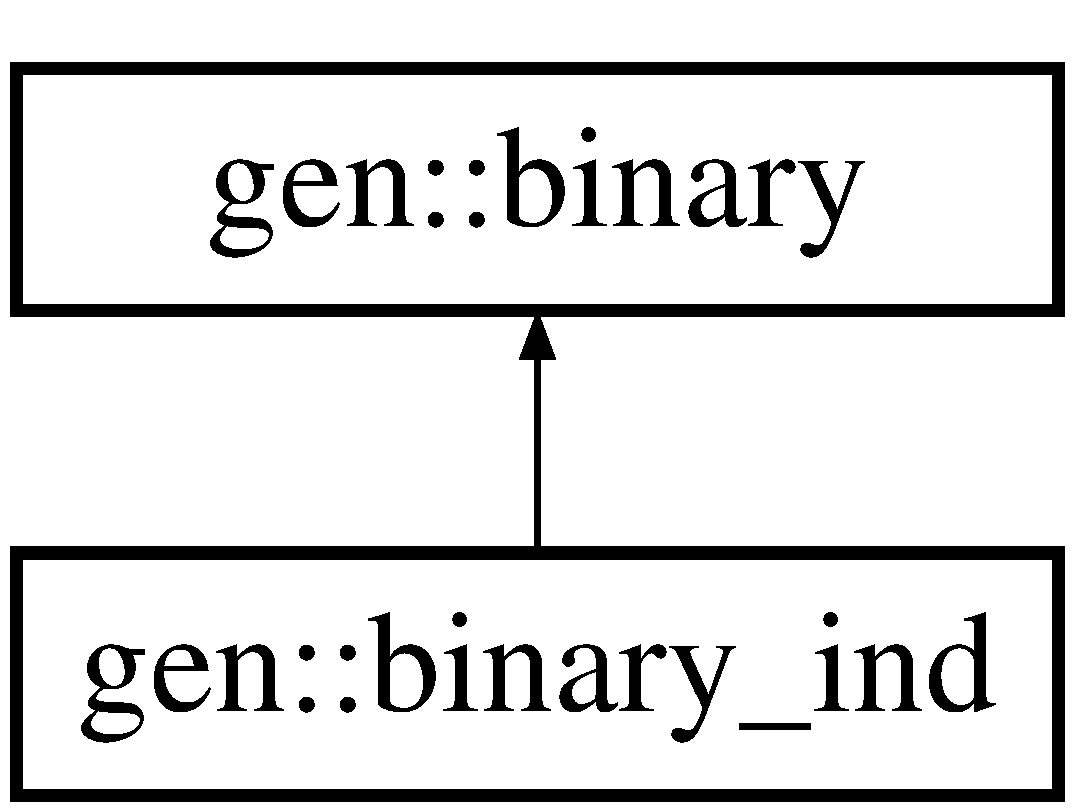
\includegraphics[height=2cm]{classgen_1_1binary__ind}
\end{center}
\end{figure}
\subsection*{Public Member Functions}
\begin{CompactItemize}
\item 
def \hyperlink{classgen_1_1binary__ind_d0e8fc3004c8d408ee9fa3b6839aa42e}{\_\-\_\-init\_\-\_\-}
\item 
def \hyperlink{classgen_1_1binary__ind_12b4f2b47589e167adfd9a96b6b522e3}{rvsplus}
\end{CompactItemize}
\subsection*{Public Attributes}
\begin{CompactItemize}
\item 
\hyperlink{classgen_1_1binary__ind_b652d5708c5922cd848116cea088ae0f}{uniform}
\item 
\hyperlink{classgen_1_1binary__ind_8f25f23a5444665383f9551a365448d0}{name}
\item 
\hyperlink{classgen_1_1binary__ind_aaf37ef74e482395cbcfb9ceaf1b564a}{p}
\end{CompactItemize}
\subsection*{Private Member Functions}
\begin{CompactItemize}
\item 
def \hyperlink{classgen_1_1binary__ind_a3f4f58e3d2b548ba7a6c23bde46f76a}{\_\-pmf}
\item 
def \hyperlink{classgen_1_1binary__ind_dad1028ef36ee6b4263db54395168586}{\_\-rvs}
\end{CompactItemize}


\subsection{Detailed Description}
Generates samples with independent components. 

\subsection{Member Function Documentation}
\hypertarget{classgen_1_1binary__ind_d0e8fc3004c8d408ee9fa3b6839aa42e}{
\index{gen::binary\_\-ind@{gen::binary\_\-ind}!\_\-\_\-init\_\-\_\-@{\_\-\_\-init\_\-\_\-}}
\index{\_\-\_\-init\_\-\_\-@{\_\-\_\-init\_\-\_\-}!gen::binary_ind@{gen::binary\_\-ind}}
\subsubsection[{\_\-\_\-init\_\-\_\-}]{\setlength{\rightskip}{0pt plus 5cm}def gen::binary\_\-ind::\_\-\_\-init\_\-\_\- ( {\em self}, \/   {\em data} = {\tt None}, \/   {\em fraction\_\-mean} = {\tt 1}, \/   {\em fraction\_\-corr} = {\tt None}, \/   {\em smooth\_\-mean} = {\tt 0}, \/   {\em smooth\_\-corr} = {\tt None}, \/   {\em threshold\_\-randomness} = {\tt 0}, \/   {\em mean} = {\tt None}, \/   {\em p} = {\tt None}, \/   {\em min\_\-p} = {\tt 0}, \/   {\em weighted} = {\tt False}, \/   {\em verbose} = {\tt False})}}
\label{classgen_1_1binary__ind_d0e8fc3004c8d408ee9fa3b6839aa42e}




Reimplemented from \hyperlink{classgen_1_1binary_705669a0b9879ed4c0f3b1d7ebac7163}{gen::binary}.\hypertarget{classgen_1_1binary__ind_a3f4f58e3d2b548ba7a6c23bde46f76a}{
\index{gen::binary\_\-ind@{gen::binary\_\-ind}!\_\-pmf@{\_\-pmf}}
\index{\_\-pmf@{\_\-pmf}!gen::binary_ind@{gen::binary\_\-ind}}
\subsubsection[{\_\-pmf}]{\setlength{\rightskip}{0pt plus 5cm}def gen::binary\_\-ind::\_\-pmf ( {\em self}, \/   {\em gamma})\hspace{0.3cm}{\tt  \mbox{[}private\mbox{]}}}}
\label{classgen_1_1binary__ind_a3f4f58e3d2b548ba7a6c23bde46f76a}


\hypertarget{classgen_1_1binary__ind_dad1028ef36ee6b4263db54395168586}{
\index{gen::binary\_\-ind@{gen::binary\_\-ind}!\_\-rvs@{\_\-rvs}}
\index{\_\-rvs@{\_\-rvs}!gen::binary_ind@{gen::binary\_\-ind}}
\subsubsection[{\_\-rvs}]{\setlength{\rightskip}{0pt plus 5cm}def gen::binary\_\-ind::\_\-rvs ( {\em self})\hspace{0.3cm}{\tt  \mbox{[}private\mbox{]}}}}
\label{classgen_1_1binary__ind_dad1028ef36ee6b4263db54395168586}


\hypertarget{classgen_1_1binary__ind_12b4f2b47589e167adfd9a96b6b522e3}{
\index{gen::binary\_\-ind@{gen::binary\_\-ind}!rvsplus@{rvsplus}}
\index{rvsplus@{rvsplus}!gen::binary_ind@{gen::binary\_\-ind}}
\subsubsection[{rvsplus}]{\setlength{\rightskip}{0pt plus 5cm}def gen::binary\_\-ind::rvsplus ( {\em self})}}
\label{classgen_1_1binary__ind_12b4f2b47589e167adfd9a96b6b522e3}




\subsection{Member Data Documentation}
\hypertarget{classgen_1_1binary__ind_8f25f23a5444665383f9551a365448d0}{
\index{gen::binary\_\-ind@{gen::binary\_\-ind}!name@{name}}
\index{name@{name}!gen::binary_ind@{gen::binary\_\-ind}}
\subsubsection[{name}]{\setlength{\rightskip}{0pt plus 5cm}{\bf gen::binary\_\-ind::name}}}
\label{classgen_1_1binary__ind_8f25f23a5444665383f9551a365448d0}


\hypertarget{classgen_1_1binary__ind_aaf37ef74e482395cbcfb9ceaf1b564a}{
\index{gen::binary\_\-ind@{gen::binary\_\-ind}!p@{p}}
\index{p@{p}!gen::binary_ind@{gen::binary\_\-ind}}
\subsubsection[{p}]{\setlength{\rightskip}{0pt plus 5cm}{\bf gen::binary\_\-ind::p}}}
\label{classgen_1_1binary__ind_aaf37ef74e482395cbcfb9ceaf1b564a}




Reimplemented from \hyperlink{classgen_1_1binary_838502808c65c543b3cb558435047f92}{gen::binary}.\hypertarget{classgen_1_1binary__ind_b652d5708c5922cd848116cea088ae0f}{
\index{gen::binary\_\-ind@{gen::binary\_\-ind}!uniform@{uniform}}
\index{uniform@{uniform}!gen::binary_ind@{gen::binary\_\-ind}}
\subsubsection[{uniform}]{\setlength{\rightskip}{0pt plus 5cm}{\bf gen::binary\_\-ind::uniform}}}
\label{classgen_1_1binary__ind_b652d5708c5922cd848116cea088ae0f}




The documentation for this class was generated from the following file:\begin{CompactItemize}
\item 
/mnt/eden/cschafer/Documents/smcdss/trunk/src/\hyperlink{gen_8py}{gen.py}\end{CompactItemize}

\hypertarget{classgen_1_1binary__log}{
\section{gen::binary\_\-log Class Reference}
\label{classgen_1_1binary__log}\index{gen::binary\_\-log@{gen::binary\_\-log}}
}
Inheritance diagram for gen::binary\_\-log::\begin{figure}[H]
\begin{center}
\leavevmode
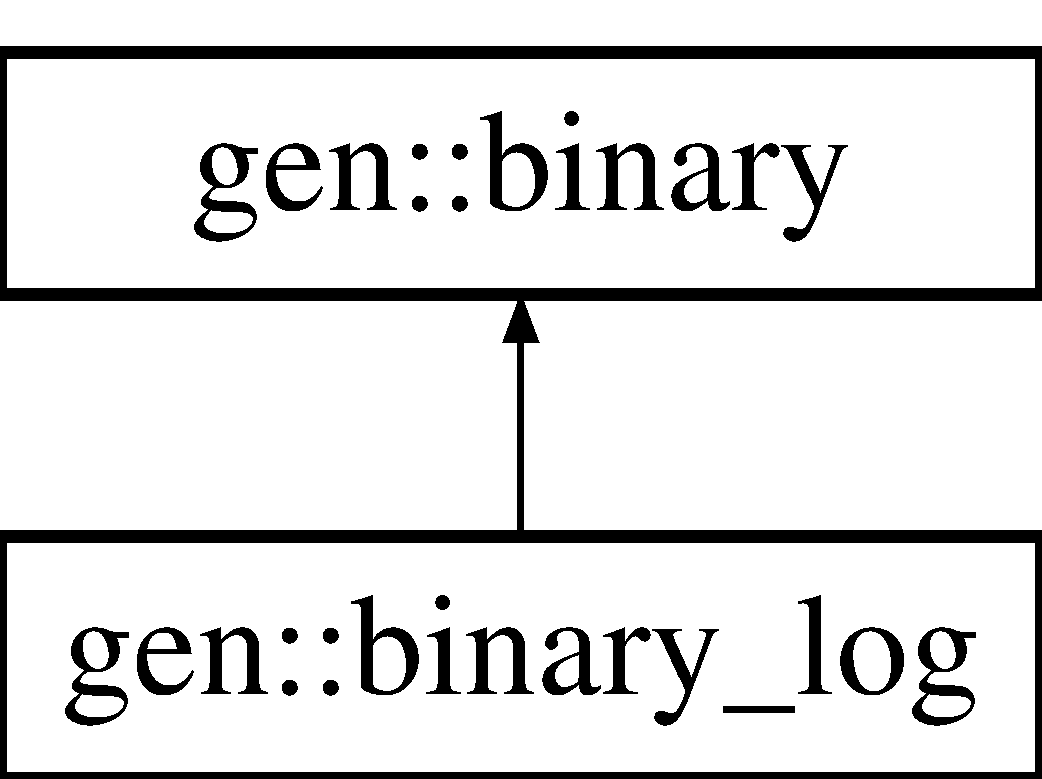
\includegraphics[height=2cm]{classgen_1_1binary__log}
\end{center}
\end{figure}
\subsection*{Public Member Functions}
\begin{CompactItemize}
\item 
def \hyperlink{classgen_1_1binary__log_46e453f2e09cc74cba4d43a8622db45f}{\_\-\_\-init\_\-\_\-}
\begin{CompactList}\small\item\em Generates samples with independent components. \item\end{CompactList}\item 
def \hyperlink{classgen_1_1binary__log_aa047299f937b4c89ae2e1fa6b9e2eac}{lpmf}
\item 
def \hyperlink{classgen_1_1binary__log_653557415fb49db33e342720fc024c21}{rvsplus}
\end{CompactItemize}
\subsection*{Public Attributes}
\begin{CompactItemize}
\item 
\hyperlink{classgen_1_1binary__log_7f23be8ef89c091c5b190ff55102090b}{name}
\item 
\hyperlink{classgen_1_1binary__log_8aec88c517667925c5e828359c2841ea}{previous\_\-betas}
\item 
\hyperlink{classgen_1_1binary__log_64b56a1380bd7d5058d2c2dbc346e4a8}{betas}
\item 
\hyperlink{classgen_1_1binary__log_2dc27524a2ecb8d70ae05dd5810aebcf}{dim}
\end{CompactItemize}
\subsection*{Private Member Functions}
\begin{CompactItemize}
\item 
def \hyperlink{classgen_1_1binary__log_9cc5e523c3d8456841c5c6354c0836c9}{\_\-pmf}
\item 
def \hyperlink{classgen_1_1binary__log_0167164fcf8820ff3be74419fac5a94c}{\_\-lpmf\_\-python}
\item 
def \hyperlink{classgen_1_1binary__log_35aba5cb13973e4a87d5e1eb14cdb8c4}{\_\-lpmf\_\-weave}
\item 
def \hyperlink{classgen_1_1binary__log_49360ebc4d0614736e8592b67b57f3d9}{\_\-rvs}
\item 
def \hyperlink{classgen_1_1binary__log_4278341c96c57b9029279a171df333ba}{\_\-rvs\_\-python}
\item 
def \hyperlink{classgen_1_1binary__log_8aac82d539642a049e2c4c8a11753f3f}{\_\-rvs\_\-weave}
\end{CompactItemize}


\subsection{Member Function Documentation}
\hypertarget{classgen_1_1binary__log_46e453f2e09cc74cba4d43a8622db45f}{
\index{gen::binary\_\-log@{gen::binary\_\-log}!\_\-\_\-init\_\-\_\-@{\_\-\_\-init\_\-\_\-}}
\index{\_\-\_\-init\_\-\_\-@{\_\-\_\-init\_\-\_\-}!gen::binary_log@{gen::binary\_\-log}}
\subsubsection[{\_\-\_\-init\_\-\_\-}]{\setlength{\rightskip}{0pt plus 5cm}def gen::binary\_\-log::\_\-\_\-init\_\-\_\- ( {\em self}, \/   {\em data} = {\tt None}, \/   {\em fraction\_\-mean} = {\tt 1}, \/   {\em smooth\_\-mean} = {\tt 0}, \/   {\em fraction\_\-corr} = {\tt 1}, \/   {\em smooth\_\-corr} = {\tt 0}, \/   {\em threshold\_\-randomness} = {\tt 0}, \/   {\em min\_\-p} = {\tt 0}, \/   {\em verbose} = {\tt False}, \/   {\em weighted} = {\tt False})}}
\label{classgen_1_1binary__log_46e453f2e09cc74cba4d43a8622db45f}


Generates samples with independent components. 

data a data object

a delay parameter b fraction for estimation log regression c mixing rate for independent samples \hypertarget{classgen_1_1binary__log_0167164fcf8820ff3be74419fac5a94c}{
\index{gen::binary\_\-log@{gen::binary\_\-log}!\_\-lpmf\_\-python@{\_\-lpmf\_\-python}}
\index{\_\-lpmf\_\-python@{\_\-lpmf\_\-python}!gen::binary_log@{gen::binary\_\-log}}
\subsubsection[{\_\-lpmf\_\-python}]{\setlength{\rightskip}{0pt plus 5cm}def gen::binary\_\-log::\_\-lpmf\_\-python ( {\em self}, \/   {\em gamma})\hspace{0.3cm}{\tt  \mbox{[}private\mbox{]}}}}
\label{classgen_1_1binary__log_0167164fcf8820ff3be74419fac5a94c}


\hypertarget{classgen_1_1binary__log_35aba5cb13973e4a87d5e1eb14cdb8c4}{
\index{gen::binary\_\-log@{gen::binary\_\-log}!\_\-lpmf\_\-weave@{\_\-lpmf\_\-weave}}
\index{\_\-lpmf\_\-weave@{\_\-lpmf\_\-weave}!gen::binary_log@{gen::binary\_\-log}}
\subsubsection[{\_\-lpmf\_\-weave}]{\setlength{\rightskip}{0pt plus 5cm}def gen::binary\_\-log::\_\-lpmf\_\-weave ( {\em self}, \/   {\em gamma})\hspace{0.3cm}{\tt  \mbox{[}private\mbox{]}}}}
\label{classgen_1_1binary__log_35aba5cb13973e4a87d5e1eb14cdb8c4}


\hypertarget{classgen_1_1binary__log_9cc5e523c3d8456841c5c6354c0836c9}{
\index{gen::binary\_\-log@{gen::binary\_\-log}!\_\-pmf@{\_\-pmf}}
\index{\_\-pmf@{\_\-pmf}!gen::binary_log@{gen::binary\_\-log}}
\subsubsection[{\_\-pmf}]{\setlength{\rightskip}{0pt plus 5cm}def gen::binary\_\-log::\_\-pmf ( {\em self}, \/   {\em gamma})\hspace{0.3cm}{\tt  \mbox{[}private\mbox{]}}}}
\label{classgen_1_1binary__log_9cc5e523c3d8456841c5c6354c0836c9}


\hypertarget{classgen_1_1binary__log_49360ebc4d0614736e8592b67b57f3d9}{
\index{gen::binary\_\-log@{gen::binary\_\-log}!\_\-rvs@{\_\-rvs}}
\index{\_\-rvs@{\_\-rvs}!gen::binary_log@{gen::binary\_\-log}}
\subsubsection[{\_\-rvs}]{\setlength{\rightskip}{0pt plus 5cm}def gen::binary\_\-log::\_\-rvs ( {\em self})\hspace{0.3cm}{\tt  \mbox{[}private\mbox{]}}}}
\label{classgen_1_1binary__log_49360ebc4d0614736e8592b67b57f3d9}


\hypertarget{classgen_1_1binary__log_4278341c96c57b9029279a171df333ba}{
\index{gen::binary\_\-log@{gen::binary\_\-log}!\_\-rvs\_\-python@{\_\-rvs\_\-python}}
\index{\_\-rvs\_\-python@{\_\-rvs\_\-python}!gen::binary_log@{gen::binary\_\-log}}
\subsubsection[{\_\-rvs\_\-python}]{\setlength{\rightskip}{0pt plus 5cm}def gen::binary\_\-log::\_\-rvs\_\-python ( {\em self})\hspace{0.3cm}{\tt  \mbox{[}private\mbox{]}}}}
\label{classgen_1_1binary__log_4278341c96c57b9029279a171df333ba}


\hypertarget{classgen_1_1binary__log_8aac82d539642a049e2c4c8a11753f3f}{
\index{gen::binary\_\-log@{gen::binary\_\-log}!\_\-rvs\_\-weave@{\_\-rvs\_\-weave}}
\index{\_\-rvs\_\-weave@{\_\-rvs\_\-weave}!gen::binary_log@{gen::binary\_\-log}}
\subsubsection[{\_\-rvs\_\-weave}]{\setlength{\rightskip}{0pt plus 5cm}def gen::binary\_\-log::\_\-rvs\_\-weave ( {\em self})\hspace{0.3cm}{\tt  \mbox{[}private\mbox{]}}}}
\label{classgen_1_1binary__log_8aac82d539642a049e2c4c8a11753f3f}


\hypertarget{classgen_1_1binary__log_aa047299f937b4c89ae2e1fa6b9e2eac}{
\index{gen::binary\_\-log@{gen::binary\_\-log}!lpmf@{lpmf}}
\index{lpmf@{lpmf}!gen::binary_log@{gen::binary\_\-log}}
\subsubsection[{lpmf}]{\setlength{\rightskip}{0pt plus 5cm}def gen::binary\_\-log::lpmf ( {\em self}, \/   {\em gamma})}}
\label{classgen_1_1binary__log_aa047299f937b4c89ae2e1fa6b9e2eac}




Reimplemented from \hyperlink{classgen_1_1binary_0377b3ffdd44806d72453d0b8ead1758}{gen::binary}.\hypertarget{classgen_1_1binary__log_653557415fb49db33e342720fc024c21}{
\index{gen::binary\_\-log@{gen::binary\_\-log}!rvsplus@{rvsplus}}
\index{rvsplus@{rvsplus}!gen::binary_log@{gen::binary\_\-log}}
\subsubsection[{rvsplus}]{\setlength{\rightskip}{0pt plus 5cm}def gen::binary\_\-log::rvsplus ( {\em self})}}
\label{classgen_1_1binary__log_653557415fb49db33e342720fc024c21}




\subsection{Member Data Documentation}
\hypertarget{classgen_1_1binary__log_64b56a1380bd7d5058d2c2dbc346e4a8}{
\index{gen::binary\_\-log@{gen::binary\_\-log}!betas@{betas}}
\index{betas@{betas}!gen::binary_log@{gen::binary\_\-log}}
\subsubsection[{betas}]{\setlength{\rightskip}{0pt plus 5cm}{\bf gen::binary\_\-log::betas}}}
\label{classgen_1_1binary__log_64b56a1380bd7d5058d2c2dbc346e4a8}


\hypertarget{classgen_1_1binary__log_2dc27524a2ecb8d70ae05dd5810aebcf}{
\index{gen::binary\_\-log@{gen::binary\_\-log}!dim@{dim}}
\index{dim@{dim}!gen::binary_log@{gen::binary\_\-log}}
\subsubsection[{dim}]{\setlength{\rightskip}{0pt plus 5cm}{\bf gen::binary\_\-log::dim}}}
\label{classgen_1_1binary__log_2dc27524a2ecb8d70ae05dd5810aebcf}




Reimplemented from \hyperlink{classgen_1_1binary_37e0504e82a2e1117ed23ff2d8617274}{gen::binary}.\hypertarget{classgen_1_1binary__log_7f23be8ef89c091c5b190ff55102090b}{
\index{gen::binary\_\-log@{gen::binary\_\-log}!name@{name}}
\index{name@{name}!gen::binary_log@{gen::binary\_\-log}}
\subsubsection[{name}]{\setlength{\rightskip}{0pt plus 5cm}{\bf gen::binary\_\-log::name}}}
\label{classgen_1_1binary__log_7f23be8ef89c091c5b190ff55102090b}


\hypertarget{classgen_1_1binary__log_8aec88c517667925c5e828359c2841ea}{
\index{gen::binary\_\-log@{gen::binary\_\-log}!previous\_\-betas@{previous\_\-betas}}
\index{previous\_\-betas@{previous\_\-betas}!gen::binary_log@{gen::binary\_\-log}}
\subsubsection[{previous\_\-betas}]{\setlength{\rightskip}{0pt plus 5cm}{\bf gen::binary\_\-log::previous\_\-betas}}}
\label{classgen_1_1binary__log_8aec88c517667925c5e828359c2841ea}




The documentation for this class was generated from the following file:\begin{CompactItemize}
\item 
/mnt/eden/cschafer/Documents/smcdss/trunk/src/\hyperlink{gen_8py}{gen.py}\end{CompactItemize}

\hypertarget{classgen_1_1binary__mn}{
\section{gen::binary\_\-mn Class Reference}
\label{classgen_1_1binary__mn}\index{gen::binary\_\-mn@{gen::binary\_\-mn}}
}
Inheritance diagram for gen::binary\_\-mn::\begin{figure}[H]
\begin{center}
\leavevmode
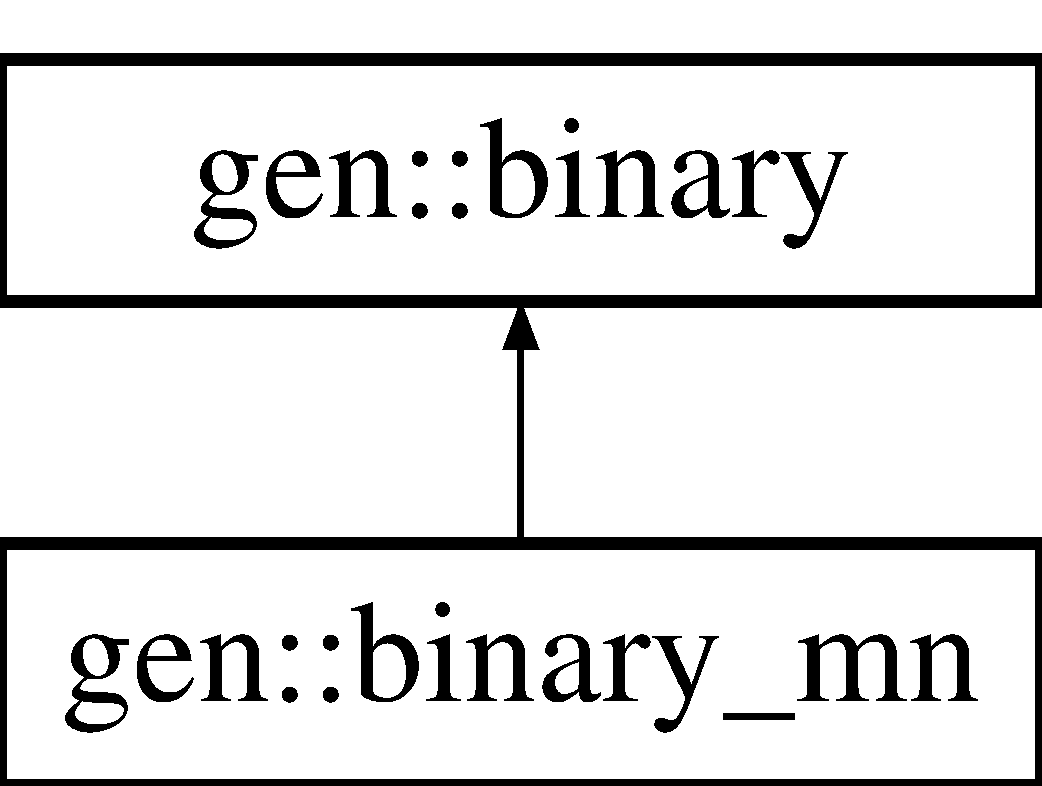
\includegraphics[height=2cm]{classgen_1_1binary__mn}
\end{center}
\end{figure}
\subsection*{Public Member Functions}
\begin{CompactItemize}
\item 
def \hyperlink{classgen_1_1binary__mn_b3ee86170c3b41948a15567440c68fac}{\_\-\_\-init\_\-\_\-}
\begin{CompactList}\small\item\em Generates samples from the multivariate normal model. \item\end{CompactList}\item 
def \hyperlink{classgen_1_1binary__mn_5c42384da221ad688d6e1a344606a017}{randomQ}
\begin{CompactList}\small\item\em Generate a random matrix X with entries U\mbox{[}-1,1\mbox{]}. \item\end{CompactList}\item 
def \hyperlink{classgen_1_1binary__mn_95f12365524907d99c52f77c36e53ba9}{independentQ}
\begin{CompactList}\small\item\em Set Q = I. \item\end{CompactList}\item 
def \hyperlink{classgen_1_1binary__mn_6e5ed2fe6e5b8c6540c797d4a49421bf}{scaledQ}
\begin{CompactList}\small\item\em Rescale the locally adjusted matrix localQ to make it positive definite. \item\end{CompactList}\item 
def \hyperlink{classgen_1_1binary__mn_98267c7b73f23c23331312345685bbee}{nearestQ}
\begin{CompactList}\small\item\em Compute the nearest correlation matrix (Frobenius norm) for the locally adjusted matrix localQ. \item\end{CompactList}\item 
def \hyperlink{classgen_1_1binary__mn_4d8919d948c2946f8c2f3a2467718ff9}{Q2R}
\begin{CompactList}\small\item\em Compute the \hyperlink{classgen_1_1binary}{binary} correlation matrix R from the normal correlation matrix Q. \item\end{CompactList}\item 
def \hyperlink{classgen_1_1binary__mn_2e6f5771808178612aefbeebe6737f18}{R2Q}
\begin{CompactList}\small\item\em Compute the locally adjusted matrix localQ from the \hyperlink{classgen_1_1binary}{binary} correlation matrix R. \item\end{CompactList}\item 
def \hyperlink{classgen_1_1binary__mn_698853fe63226716476aa5a4bf9df76c}{R2localQ}
\begin{CompactList}\small\item\em Compute the locally adjusted matrix localQ from the \hyperlink{classgen_1_1binary}{binary} correlation matrix R. \item\end{CompactList}\item 
def \hyperlink{classgen_1_1binary__mn_f8d4b9ee7e9ed2ed06c4da3b2babaadf}{r2localq}
\begin{CompactList}\small\item\em Computes the normal correlation q necessary to generate a bivariate bernoulli samples with correlation r. \item\end{CompactList}\end{CompactItemize}
\subsection*{Public Attributes}
\begin{CompactItemize}
\item 
\hyperlink{classgen_1_1binary__mn_3a53b153bb420c5888eb0e65047bf3db}{name}
\item 
\hyperlink{classgen_1_1binary__mn_1df80ef0ecd8ba01ec9a6a2a460f46cc}{oldC}
\item 
\hyperlink{classgen_1_1binary__mn_60a38465bb9902b0fce51973efb4f65a}{oldQ}
\item 
\hyperlink{classgen_1_1binary__mn_bac8dcefdbdb3f0ec22628023041e779}{oldmu}
\item 
\hyperlink{classgen_1_1binary__mn_dc21a4441917a15c0336211938051cac}{data}
\item 
\hyperlink{classgen_1_1binary__mn_a3e93467420a3516765e31ecd164808f}{R}
\item 
\hyperlink{classgen_1_1binary__mn_eaff316a00faac4a925e5fc2a9ae8b59}{mean}
\item 
\hyperlink{classgen_1_1binary__mn_31f2c16e8843c761fbd4dcbd0d4237ed}{mu}
\item 
\hyperlink{classgen_1_1binary__mn_cb44e6b25ddd534c843734c4443c2f21}{p}
\item 
\hyperlink{classgen_1_1binary__mn_26e659ee26e9a63f034065231014f3a3}{Q}
\item 
\hyperlink{classgen_1_1binary__mn_30427a1bc1bbc9f50e67e20d763c9c1e}{C}
\item 
\hyperlink{classgen_1_1binary__mn_878160281d5c61d8de14db9ebc93f822}{dim}
\end{CompactItemize}
\subsection*{Static Public Attributes}
\begin{CompactItemize}
\item 
tuple \hyperlink{classgen_1_1binary__mn_e27aacf71cc73e5a334eb14344706ddc}{r2localq} = staticmethod(\hyperlink{classgen_1_1binary__mn_e27aacf71cc73e5a334eb14344706ddc}{r2localq})
\end{CompactItemize}
\subsection*{Private Member Functions}
\begin{CompactItemize}
\item 
def \hyperlink{classgen_1_1binary__mn_a6f0dd2bcf5dc7087ce71b982408a963}{\_\-pmf}
\item 
def \hyperlink{classgen_1_1binary__mn_281d5cb707dd1b6845c3aa9d63a5558e}{\_\-rvs}
\end{CompactItemize}


\subsection{Member Function Documentation}
\hypertarget{classgen_1_1binary__mn_b3ee86170c3b41948a15567440c68fac}{
\index{gen::binary\_\-mn@{gen::binary\_\-mn}!\_\-\_\-init\_\-\_\-@{\_\-\_\-init\_\-\_\-}}
\index{\_\-\_\-init\_\-\_\-@{\_\-\_\-init\_\-\_\-}!gen::binary_mn@{gen::binary\_\-mn}}
\subsubsection[{\_\-\_\-init\_\-\_\-}]{\setlength{\rightskip}{0pt plus 5cm}def gen::binary\_\-mn::\_\-\_\-init\_\-\_\- ( {\em self}, \/   {\em data} = {\tt None}, \/   {\em fraction\_\-mean} = {\tt 1}, \/   {\em smooth\_\-mean} = {\tt 0}, \/   {\em fraction\_\-corr} = {\tt 1}, \/   {\em smooth\_\-corr} = {\tt 0}, \/   {\em threshold\_\-randomness} = {\tt 0}, \/   {\em mu} = {\tt \char`\"{}random\char`\"{}}, \/   {\em Q} = {\tt \char`\"{}independent\char`\"{}}, \/   {\em mean} = {\tt None}, \/   {\em R} = {\tt None}, \/   {\em p} = {\tt None}, \/   {\em min\_\-p} = {\tt 0}, \/   {\em weighted} = {\tt False}, \/   {\em verbose} = {\tt False})}}
\label{classgen_1_1binary__mn_b3ee86170c3b41948a15567440c68fac}


Generates samples from the multivariate normal model. 

data data object mu mean vector (normal) Q correlation matrix (normal) mean probability vector (\hyperlink{classgen_1_1binary}{binary}) R correlation matrix (\hyperlink{classgen_1_1binary}{binary}) p dimension

a delay parameter b fraction for estimation of R c decrease correlation by R = (c$\ast$I+R)/(1+c)

mu = \char`\"{}uniform\char`\"{}, \char`\"{}random\char`\"{} Q = \char`\"{}scaled\char`\"{}, \char`\"{}nearest\char`\"{}, \char`\"{}gaussian\char`\"{}, \char`\"{}independent\char`\"{}, \char`\"{}random\char`\"{} \hypertarget{classgen_1_1binary__mn_a6f0dd2bcf5dc7087ce71b982408a963}{
\index{gen::binary\_\-mn@{gen::binary\_\-mn}!\_\-pmf@{\_\-pmf}}
\index{\_\-pmf@{\_\-pmf}!gen::binary_mn@{gen::binary\_\-mn}}
\subsubsection[{\_\-pmf}]{\setlength{\rightskip}{0pt plus 5cm}def gen::binary\_\-mn::\_\-pmf ( {\em self}, \/   {\em gamma})\hspace{0.3cm}{\tt  \mbox{[}private\mbox{]}}}}
\label{classgen_1_1binary__mn_a6f0dd2bcf5dc7087ce71b982408a963}


\hypertarget{classgen_1_1binary__mn_281d5cb707dd1b6845c3aa9d63a5558e}{
\index{gen::binary\_\-mn@{gen::binary\_\-mn}!\_\-rvs@{\_\-rvs}}
\index{\_\-rvs@{\_\-rvs}!gen::binary_mn@{gen::binary\_\-mn}}
\subsubsection[{\_\-rvs}]{\setlength{\rightskip}{0pt plus 5cm}def gen::binary\_\-mn::\_\-rvs ( {\em self})\hspace{0.3cm}{\tt  \mbox{[}private\mbox{]}}}}
\label{classgen_1_1binary__mn_281d5cb707dd1b6845c3aa9d63a5558e}


\hypertarget{classgen_1_1binary__mn_95f12365524907d99c52f77c36e53ba9}{
\index{gen::binary\_\-mn@{gen::binary\_\-mn}!independentQ@{independentQ}}
\index{independentQ@{independentQ}!gen::binary_mn@{gen::binary\_\-mn}}
\subsubsection[{independentQ}]{\setlength{\rightskip}{0pt plus 5cm}def gen::binary\_\-mn::independentQ ( {\em self})}}
\label{classgen_1_1binary__mn_95f12365524907d99c52f77c36e53ba9}


Set Q = I. 

\hypertarget{classgen_1_1binary__mn_98267c7b73f23c23331312345685bbee}{
\index{gen::binary\_\-mn@{gen::binary\_\-mn}!nearestQ@{nearestQ}}
\index{nearestQ@{nearestQ}!gen::binary_mn@{gen::binary\_\-mn}}
\subsubsection[{nearestQ}]{\setlength{\rightskip}{0pt plus 5cm}def gen::binary\_\-mn::nearestQ ( {\em self})}}
\label{classgen_1_1binary__mn_98267c7b73f23c23331312345685bbee}


Compute the nearest correlation matrix (Frobenius norm) for the locally adjusted matrix localQ. 

The nearest correlation matrix problem is solved using the alternating projection method proposed in \char`\"{}Computing the Nearest Correlation Matrix - A problem from Finance\char`\"{} by N. Higham (2001) \hypertarget{classgen_1_1binary__mn_4d8919d948c2946f8c2f3a2467718ff9}{
\index{gen::binary\_\-mn@{gen::binary\_\-mn}!Q2R@{Q2R}}
\index{Q2R@{Q2R}!gen::binary_mn@{gen::binary\_\-mn}}
\subsubsection[{Q2R}]{\setlength{\rightskip}{0pt plus 5cm}def gen::binary\_\-mn::Q2R ( {\em self})}}
\label{classgen_1_1binary__mn_4d8919d948c2946f8c2f3a2467718ff9}


Compute the \hyperlink{classgen_1_1binary}{binary} correlation matrix R from the normal correlation matrix Q. 

\hypertarget{classgen_1_1binary__mn_f8d4b9ee7e9ed2ed06c4da3b2babaadf}{
\index{gen::binary\_\-mn@{gen::binary\_\-mn}!r2localq@{r2localq}}
\index{r2localq@{r2localq}!gen::binary_mn@{gen::binary\_\-mn}}
\subsubsection[{r2localq}]{\setlength{\rightskip}{0pt plus 5cm}def {\bf gen::binary\_\-mn::r2localq} ( {\em mu}, \/   {\em rho}, \/   {\em p} = {\tt \mbox{[}inf}, \/   {\em inf}, \/   {\em initq} = {\tt 0}, \/   {\em verbose} = {\tt False})}}
\label{classgen_1_1binary__mn_f8d4b9ee7e9ed2ed06c4da3b2babaadf}


Computes the normal correlation q necessary to generate a bivariate bernoulli samples with correlation r. 

mu mean of normal variates r target correlation of bernoulli variates p mean of bianry variates \hypertarget{classgen_1_1binary__mn_698853fe63226716476aa5a4bf9df76c}{
\index{gen::binary\_\-mn@{gen::binary\_\-mn}!R2localQ@{R2localQ}}
\index{R2localQ@{R2localQ}!gen::binary_mn@{gen::binary\_\-mn}}
\subsubsection[{R2localQ}]{\setlength{\rightskip}{0pt plus 5cm}def gen::binary\_\-mn::R2localQ ( {\em self})}}
\label{classgen_1_1binary__mn_698853fe63226716476aa5a4bf9df76c}


Compute the locally adjusted matrix localQ from the \hyperlink{classgen_1_1binary}{binary} correlation matrix R. 

\hypertarget{classgen_1_1binary__mn_2e6f5771808178612aefbeebe6737f18}{
\index{gen::binary\_\-mn@{gen::binary\_\-mn}!R2Q@{R2Q}}
\index{R2Q@{R2Q}!gen::binary_mn@{gen::binary\_\-mn}}
\subsubsection[{R2Q}]{\setlength{\rightskip}{0pt plus 5cm}def gen::binary\_\-mn::R2Q ( {\em self})}}
\label{classgen_1_1binary__mn_2e6f5771808178612aefbeebe6737f18}


Compute the locally adjusted matrix localQ from the \hyperlink{classgen_1_1binary}{binary} correlation matrix R. 

\hypertarget{classgen_1_1binary__mn_5c42384da221ad688d6e1a344606a017}{
\index{gen::binary\_\-mn@{gen::binary\_\-mn}!randomQ@{randomQ}}
\index{randomQ@{randomQ}!gen::binary_mn@{gen::binary\_\-mn}}
\subsubsection[{randomQ}]{\setlength{\rightskip}{0pt plus 5cm}def gen::binary\_\-mn::randomQ ( {\em self})}}
\label{classgen_1_1binary__mn_5c42384da221ad688d6e1a344606a017}


Generate a random matrix X with entries U\mbox{[}-1,1\mbox{]}. 

Set Q = X$\ast$X$^\wedge$t and normalize. \hypertarget{classgen_1_1binary__mn_6e5ed2fe6e5b8c6540c797d4a49421bf}{
\index{gen::binary\_\-mn@{gen::binary\_\-mn}!scaledQ@{scaledQ}}
\index{scaledQ@{scaledQ}!gen::binary_mn@{gen::binary\_\-mn}}
\subsubsection[{scaledQ}]{\setlength{\rightskip}{0pt plus 5cm}def gen::binary\_\-mn::scaledQ ( {\em self})}}
\label{classgen_1_1binary__mn_6e5ed2fe6e5b8c6540c797d4a49421bf}


Rescale the locally adjusted matrix localQ to make it positive definite. 



\subsection{Member Data Documentation}
\hypertarget{classgen_1_1binary__mn_30427a1bc1bbc9f50e67e20d763c9c1e}{
\index{gen::binary\_\-mn@{gen::binary\_\-mn}!C@{C}}
\index{C@{C}!gen::binary_mn@{gen::binary\_\-mn}}
\subsubsection[{C}]{\setlength{\rightskip}{0pt plus 5cm}{\bf gen::binary\_\-mn::C}}}
\label{classgen_1_1binary__mn_30427a1bc1bbc9f50e67e20d763c9c1e}


\hypertarget{classgen_1_1binary__mn_dc21a4441917a15c0336211938051cac}{
\index{gen::binary\_\-mn@{gen::binary\_\-mn}!data@{data}}
\index{data@{data}!gen::binary_mn@{gen::binary\_\-mn}}
\subsubsection[{data}]{\setlength{\rightskip}{0pt plus 5cm}{\bf gen::binary\_\-mn::data}}}
\label{classgen_1_1binary__mn_dc21a4441917a15c0336211938051cac}




Reimplemented from \hyperlink{classgen_1_1binary_156a3b3004ee18dc4472dbbb22e58441}{gen::binary}.\hypertarget{classgen_1_1binary__mn_878160281d5c61d8de14db9ebc93f822}{
\index{gen::binary\_\-mn@{gen::binary\_\-mn}!dim@{dim}}
\index{dim@{dim}!gen::binary_mn@{gen::binary\_\-mn}}
\subsubsection[{dim}]{\setlength{\rightskip}{0pt plus 5cm}{\bf gen::binary\_\-mn::dim}}}
\label{classgen_1_1binary__mn_878160281d5c61d8de14db9ebc93f822}




Reimplemented from \hyperlink{classgen_1_1binary_37e0504e82a2e1117ed23ff2d8617274}{gen::binary}.\hypertarget{classgen_1_1binary__mn_eaff316a00faac4a925e5fc2a9ae8b59}{
\index{gen::binary\_\-mn@{gen::binary\_\-mn}!mean@{mean}}
\index{mean@{mean}!gen::binary_mn@{gen::binary\_\-mn}}
\subsubsection[{mean}]{\setlength{\rightskip}{0pt plus 5cm}{\bf gen::binary\_\-mn::mean}}}
\label{classgen_1_1binary__mn_eaff316a00faac4a925e5fc2a9ae8b59}




Reimplemented from \hyperlink{classgen_1_1binary_a14a164be1fc67e5a014782fc29d287b}{gen::binary}.\hypertarget{classgen_1_1binary__mn_31f2c16e8843c761fbd4dcbd0d4237ed}{
\index{gen::binary\_\-mn@{gen::binary\_\-mn}!mu@{mu}}
\index{mu@{mu}!gen::binary_mn@{gen::binary\_\-mn}}
\subsubsection[{mu}]{\setlength{\rightskip}{0pt plus 5cm}{\bf gen::binary\_\-mn::mu}}}
\label{classgen_1_1binary__mn_31f2c16e8843c761fbd4dcbd0d4237ed}


\hypertarget{classgen_1_1binary__mn_3a53b153bb420c5888eb0e65047bf3db}{
\index{gen::binary\_\-mn@{gen::binary\_\-mn}!name@{name}}
\index{name@{name}!gen::binary_mn@{gen::binary\_\-mn}}
\subsubsection[{name}]{\setlength{\rightskip}{0pt plus 5cm}{\bf gen::binary\_\-mn::name}}}
\label{classgen_1_1binary__mn_3a53b153bb420c5888eb0e65047bf3db}


\hypertarget{classgen_1_1binary__mn_1df80ef0ecd8ba01ec9a6a2a460f46cc}{
\index{gen::binary\_\-mn@{gen::binary\_\-mn}!oldC@{oldC}}
\index{oldC@{oldC}!gen::binary_mn@{gen::binary\_\-mn}}
\subsubsection[{oldC}]{\setlength{\rightskip}{0pt plus 5cm}{\bf gen::binary\_\-mn::oldC}}}
\label{classgen_1_1binary__mn_1df80ef0ecd8ba01ec9a6a2a460f46cc}


\hypertarget{classgen_1_1binary__mn_bac8dcefdbdb3f0ec22628023041e779}{
\index{gen::binary\_\-mn@{gen::binary\_\-mn}!oldmu@{oldmu}}
\index{oldmu@{oldmu}!gen::binary_mn@{gen::binary\_\-mn}}
\subsubsection[{oldmu}]{\setlength{\rightskip}{0pt plus 5cm}{\bf gen::binary\_\-mn::oldmu}}}
\label{classgen_1_1binary__mn_bac8dcefdbdb3f0ec22628023041e779}


\hypertarget{classgen_1_1binary__mn_60a38465bb9902b0fce51973efb4f65a}{
\index{gen::binary\_\-mn@{gen::binary\_\-mn}!oldQ@{oldQ}}
\index{oldQ@{oldQ}!gen::binary_mn@{gen::binary\_\-mn}}
\subsubsection[{oldQ}]{\setlength{\rightskip}{0pt plus 5cm}{\bf gen::binary\_\-mn::oldQ}}}
\label{classgen_1_1binary__mn_60a38465bb9902b0fce51973efb4f65a}


\hypertarget{classgen_1_1binary__mn_cb44e6b25ddd534c843734c4443c2f21}{
\index{gen::binary\_\-mn@{gen::binary\_\-mn}!p@{p}}
\index{p@{p}!gen::binary_mn@{gen::binary\_\-mn}}
\subsubsection[{p}]{\setlength{\rightskip}{0pt plus 5cm}{\bf gen::binary\_\-mn::p}}}
\label{classgen_1_1binary__mn_cb44e6b25ddd534c843734c4443c2f21}




Reimplemented from \hyperlink{classgen_1_1binary_838502808c65c543b3cb558435047f92}{gen::binary}.\hypertarget{classgen_1_1binary__mn_26e659ee26e9a63f034065231014f3a3}{
\index{gen::binary\_\-mn@{gen::binary\_\-mn}!Q@{Q}}
\index{Q@{Q}!gen::binary_mn@{gen::binary\_\-mn}}
\subsubsection[{Q}]{\setlength{\rightskip}{0pt plus 5cm}{\bf gen::binary\_\-mn::Q}}}
\label{classgen_1_1binary__mn_26e659ee26e9a63f034065231014f3a3}


\hypertarget{classgen_1_1binary__mn_a3e93467420a3516765e31ecd164808f}{
\index{gen::binary\_\-mn@{gen::binary\_\-mn}!R@{R}}
\index{R@{R}!gen::binary_mn@{gen::binary\_\-mn}}
\subsubsection[{R}]{\setlength{\rightskip}{0pt plus 5cm}{\bf gen::binary\_\-mn::R}}}
\label{classgen_1_1binary__mn_a3e93467420a3516765e31ecd164808f}


\hypertarget{classgen_1_1binary__mn_e27aacf71cc73e5a334eb14344706ddc}{
\index{gen::binary\_\-mn@{gen::binary\_\-mn}!r2localq@{r2localq}}
\index{r2localq@{r2localq}!gen::binary_mn@{gen::binary\_\-mn}}
\subsubsection[{r2localq}]{\setlength{\rightskip}{0pt plus 5cm}tuple {\bf gen::binary\_\-mn::r2localq} = staticmethod({\bf r2localq})\hspace{0.3cm}{\tt  \mbox{[}static\mbox{]}}}}
\label{classgen_1_1binary__mn_e27aacf71cc73e5a334eb14344706ddc}




The documentation for this class was generated from the following file:\begin{CompactItemize}
\item 
/mnt/eden/cschafer/Documents/smcdss/trunk/src/\hyperlink{gen_8py}{gen.py}\end{CompactItemize}

\hypertarget{classgen_1_1binary__post}{
\section{gen::binary\_\-post Class Reference}
\label{classgen_1_1binary__post}\index{gen::binary\_\-post@{gen::binary\_\-post}}
}
Inheritance diagram for gen::binary\_\-post::\begin{figure}[H]
\begin{center}
\leavevmode
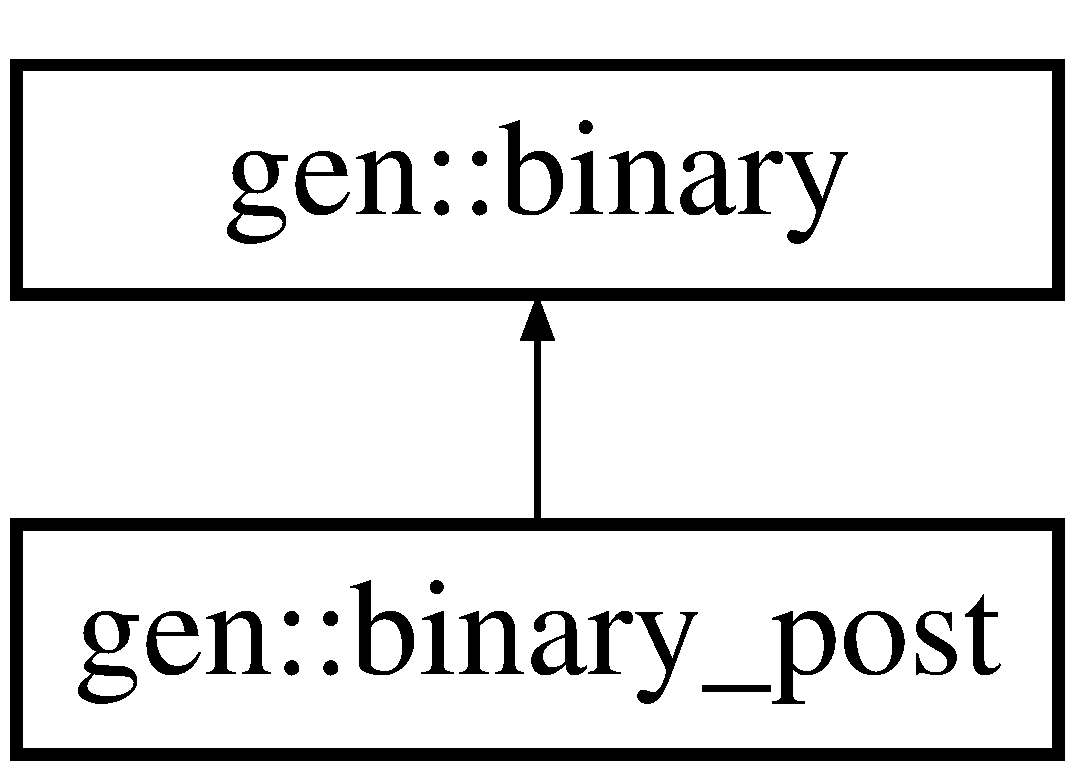
\includegraphics[height=2cm]{classgen_1_1binary__post}
\end{center}
\end{figure}
\subsection*{Public Member Functions}
\begin{CompactItemize}
\item 
def \hyperlink{classgen_1_1binary__post_7069c5816dfa311016a8ea94494ae99f}{\_\-\_\-init\_\-\_\-}
\begin{CompactList}\small\item\em Reads a dataset and construct the posterior probabilities of all linear models with variates regressed on the first column. \item\end{CompactList}\item 
def \hyperlink{classgen_1_1binary__post_2ad20ce2b2b31381d879c8f83559f771}{lpmf}
\begin{CompactList}\small\item\em Evaluates the unnormalized log pmf. \item\end{CompactList}\item 
def \hyperlink{classgen_1_1binary__post_26a109b16742daa55d257a7678e156c3}{hb}
\begin{CompactList}\small\item\em Evaluates the log posterior density from a conjugate hierarchical setup (\mbox{[}George, McCulloch 1997\mbox{]}, simplified). \item\end{CompactList}\item 
def \hyperlink{classgen_1_1binary__post_f34f5b3a16fe5f6b90b61feac26a759c}{bic}
\begin{CompactList}\small\item\em Evaluates the Bayesian Information Criterion. \item\end{CompactList}\end{CompactItemize}
\subsection*{Public Attributes}
\begin{CompactItemize}
\item 
\hyperlink{classgen_1_1binary__post_7f257df286a4acedfc26064cb3db0661}{name}
\item 
\hyperlink{classgen_1_1binary__post_c4a4e7585d9ec429e5a8ad9998d15ba7}{scoretype}
\item 
\hyperlink{classgen_1_1binary__post_f6b86842ca928b27461adcb6f3800cf6}{dim}
\item 
\hyperlink{classgen_1_1binary__post_07f91fffaa967ad5191151bf512f073f}{feasible}
\item 
\hyperlink{classgen_1_1binary__post_28e8dd27262ae15d0151c4ab614c5807}{n}
\item 
\hyperlink{classgen_1_1binary__post_5569d4727af98880ab6efd2baecc943f}{XtY}
\item 
\hyperlink{classgen_1_1binary__post_0ba4dc90f0854325754b5002f9d1f3f6}{XtX}
\item 
\hyperlink{classgen_1_1binary__post_419c9831e2edd73f7eea540fc4ac1839}{c1}
\item 
\hyperlink{classgen_1_1binary__post_11f0ba4507df919b0b30d9644c22f475}{c2}
\item 
\hyperlink{classgen_1_1binary__post_cafd9471ff9337bbb8b2ad9f4b822963}{c3}
\item 
\hyperlink{classgen_1_1binary__post_1f3e1139fe6a08a79f7f223705f7e207}{loglevel}
\end{CompactItemize}
\subsection*{Private Member Functions}
\begin{CompactItemize}
\item 
def \hyperlink{classgen_1_1binary__post_a599045ffd56b46eced7ebae979781ff}{\_\-pmf}
\begin{CompactList}\small\item\em Evaluates unnormalized pmf. \item\end{CompactList}\item 
def \hyperlink{classgen_1_1binary__post_fbfecb84772369428033234930e079a8}{\_\-explore}
\begin{CompactList}\small\item\em Find the maximmum of the log posterior for feasible dimensions. \item\end{CompactList}\item 
def \hyperlink{classgen_1_1binary__post_bc265fbdb0840423716d8a4904469ac8}{\_\-rvs}
\begin{CompactList}\small\item\em Generates a sample from the posterior density rejecting from a proposals of independent 0.5-binary variables. \item\end{CompactList}\end{CompactItemize}


\subsection{Member Function Documentation}
\hypertarget{classgen_1_1binary__post_7069c5816dfa311016a8ea94494ae99f}{
\index{gen::binary\_\-post@{gen::binary\_\-post}!\_\-\_\-init\_\-\_\-@{\_\-\_\-init\_\-\_\-}}
\index{\_\-\_\-init\_\-\_\-@{\_\-\_\-init\_\-\_\-}!gen::binary_post@{gen::binary\_\-post}}
\subsubsection[{\_\-\_\-init\_\-\_\-}]{\setlength{\rightskip}{0pt plus 5cm}def gen::binary\_\-post::\_\-\_\-init\_\-\_\- ( {\em self}, \/   {\em dataset}, \/   {\em scoretype} = {\tt 'hb'})}}
\label{classgen_1_1binary__post_7069c5816dfa311016a8ea94494ae99f}


Reads a dataset and construct the posterior probabilities of all linear models with variates regressed on the first column. 

\hypertarget{classgen_1_1binary__post_fbfecb84772369428033234930e079a8}{
\index{gen::binary\_\-post@{gen::binary\_\-post}!\_\-explore@{\_\-explore}}
\index{\_\-explore@{\_\-explore}!gen::binary_post@{gen::binary\_\-post}}
\subsubsection[{\_\-explore}]{\setlength{\rightskip}{0pt plus 5cm}def gen::binary\_\-post::\_\-explore ( {\em self})\hspace{0.3cm}{\tt  \mbox{[}private\mbox{]}}}}
\label{classgen_1_1binary__post_fbfecb84772369428033234930e079a8}


Find the maximmum of the log posterior for feasible dimensions. 

\hypertarget{classgen_1_1binary__post_a599045ffd56b46eced7ebae979781ff}{
\index{gen::binary\_\-post@{gen::binary\_\-post}!\_\-pmf@{\_\-pmf}}
\index{\_\-pmf@{\_\-pmf}!gen::binary_post@{gen::binary\_\-post}}
\subsubsection[{\_\-pmf}]{\setlength{\rightskip}{0pt plus 5cm}def gen::binary\_\-post::\_\-pmf ( {\em self}, \/   {\em gamma})\hspace{0.3cm}{\tt  \mbox{[}private\mbox{]}}}}
\label{classgen_1_1binary__post_a599045ffd56b46eced7ebae979781ff}


Evaluates unnormalized pmf. 

gamma a \hyperlink{classgen_1_1binary}{binary} vector of length p \hypertarget{classgen_1_1binary__post_bc265fbdb0840423716d8a4904469ac8}{
\index{gen::binary\_\-post@{gen::binary\_\-post}!\_\-rvs@{\_\-rvs}}
\index{\_\-rvs@{\_\-rvs}!gen::binary_post@{gen::binary\_\-post}}
\subsubsection[{\_\-rvs}]{\setlength{\rightskip}{0pt plus 5cm}def gen::binary\_\-post::\_\-rvs ( {\em self})\hspace{0.3cm}{\tt  \mbox{[}private\mbox{]}}}}
\label{classgen_1_1binary__post_bc265fbdb0840423716d8a4904469ac8}


Generates a sample from the posterior density rejecting from a proposals of independent 0.5-binary variables. 

\hypertarget{classgen_1_1binary__post_f34f5b3a16fe5f6b90b61feac26a759c}{
\index{gen::binary\_\-post@{gen::binary\_\-post}!bic@{bic}}
\index{bic@{bic}!gen::binary_post@{gen::binary\_\-post}}
\subsubsection[{bic}]{\setlength{\rightskip}{0pt plus 5cm}def gen::binary\_\-post::bic ( {\em self}, \/   {\em gamma})}}
\label{classgen_1_1binary__post_f34f5b3a16fe5f6b90b61feac26a759c}


Evaluates the Bayesian Information Criterion. 

gamma a \hyperlink{classgen_1_1binary}{binary} vector \hypertarget{classgen_1_1binary__post_26a109b16742daa55d257a7678e156c3}{
\index{gen::binary\_\-post@{gen::binary\_\-post}!hb@{hb}}
\index{hb@{hb}!gen::binary_post@{gen::binary\_\-post}}
\subsubsection[{hb}]{\setlength{\rightskip}{0pt plus 5cm}def gen::binary\_\-post::hb ( {\em self}, \/   {\em gamma})}}
\label{classgen_1_1binary__post_26a109b16742daa55d257a7678e156c3}


Evaluates the log posterior density from a conjugate hierarchical setup (\mbox{[}George, McCulloch 1997\mbox{]}, simplified). 

gamma a \hyperlink{classgen_1_1binary}{binary} vector \hypertarget{classgen_1_1binary__post_2ad20ce2b2b31381d879c8f83559f771}{
\index{gen::binary\_\-post@{gen::binary\_\-post}!lpmf@{lpmf}}
\index{lpmf@{lpmf}!gen::binary_post@{gen::binary\_\-post}}
\subsubsection[{lpmf}]{\setlength{\rightskip}{0pt plus 5cm}def gen::binary\_\-post::lpmf ( {\em self}, \/   {\em gamma})}}
\label{classgen_1_1binary__post_2ad20ce2b2b31381d879c8f83559f771}


Evaluates the unnormalized log pmf. 

gamma a \hyperlink{classgen_1_1binary}{binary} vector 

Reimplemented from \hyperlink{classgen_1_1binary_0377b3ffdd44806d72453d0b8ead1758}{gen::binary}.

\subsection{Member Data Documentation}
\hypertarget{classgen_1_1binary__post_419c9831e2edd73f7eea540fc4ac1839}{
\index{gen::binary\_\-post@{gen::binary\_\-post}!c1@{c1}}
\index{c1@{c1}!gen::binary_post@{gen::binary\_\-post}}
\subsubsection[{c1}]{\setlength{\rightskip}{0pt plus 5cm}{\bf gen::binary\_\-post::c1}}}
\label{classgen_1_1binary__post_419c9831e2edd73f7eea540fc4ac1839}


\hypertarget{classgen_1_1binary__post_11f0ba4507df919b0b30d9644c22f475}{
\index{gen::binary\_\-post@{gen::binary\_\-post}!c2@{c2}}
\index{c2@{c2}!gen::binary_post@{gen::binary\_\-post}}
\subsubsection[{c2}]{\setlength{\rightskip}{0pt plus 5cm}{\bf gen::binary\_\-post::c2}}}
\label{classgen_1_1binary__post_11f0ba4507df919b0b30d9644c22f475}


\hypertarget{classgen_1_1binary__post_cafd9471ff9337bbb8b2ad9f4b822963}{
\index{gen::binary\_\-post@{gen::binary\_\-post}!c3@{c3}}
\index{c3@{c3}!gen::binary_post@{gen::binary\_\-post}}
\subsubsection[{c3}]{\setlength{\rightskip}{0pt plus 5cm}{\bf gen::binary\_\-post::c3}}}
\label{classgen_1_1binary__post_cafd9471ff9337bbb8b2ad9f4b822963}


\hypertarget{classgen_1_1binary__post_f6b86842ca928b27461adcb6f3800cf6}{
\index{gen::binary\_\-post@{gen::binary\_\-post}!dim@{dim}}
\index{dim@{dim}!gen::binary_post@{gen::binary\_\-post}}
\subsubsection[{dim}]{\setlength{\rightskip}{0pt plus 5cm}{\bf gen::binary\_\-post::dim}}}
\label{classgen_1_1binary__post_f6b86842ca928b27461adcb6f3800cf6}




Reimplemented from \hyperlink{classgen_1_1binary_37e0504e82a2e1117ed23ff2d8617274}{gen::binary}.\hypertarget{classgen_1_1binary__post_07f91fffaa967ad5191151bf512f073f}{
\index{gen::binary\_\-post@{gen::binary\_\-post}!feasible@{feasible}}
\index{feasible@{feasible}!gen::binary_post@{gen::binary\_\-post}}
\subsubsection[{feasible}]{\setlength{\rightskip}{0pt plus 5cm}{\bf gen::binary\_\-post::feasible}}}
\label{classgen_1_1binary__post_07f91fffaa967ad5191151bf512f073f}


\hypertarget{classgen_1_1binary__post_1f3e1139fe6a08a79f7f223705f7e207}{
\index{gen::binary\_\-post@{gen::binary\_\-post}!loglevel@{loglevel}}
\index{loglevel@{loglevel}!gen::binary_post@{gen::binary\_\-post}}
\subsubsection[{loglevel}]{\setlength{\rightskip}{0pt plus 5cm}{\bf gen::binary\_\-post::loglevel}}}
\label{classgen_1_1binary__post_1f3e1139fe6a08a79f7f223705f7e207}


\hypertarget{classgen_1_1binary__post_28e8dd27262ae15d0151c4ab614c5807}{
\index{gen::binary\_\-post@{gen::binary\_\-post}!n@{n}}
\index{n@{n}!gen::binary_post@{gen::binary\_\-post}}
\subsubsection[{n}]{\setlength{\rightskip}{0pt plus 5cm}{\bf gen::binary\_\-post::n}}}
\label{classgen_1_1binary__post_28e8dd27262ae15d0151c4ab614c5807}


\hypertarget{classgen_1_1binary__post_7f257df286a4acedfc26064cb3db0661}{
\index{gen::binary\_\-post@{gen::binary\_\-post}!name@{name}}
\index{name@{name}!gen::binary_post@{gen::binary\_\-post}}
\subsubsection[{name}]{\setlength{\rightskip}{0pt plus 5cm}{\bf gen::binary\_\-post::name}}}
\label{classgen_1_1binary__post_7f257df286a4acedfc26064cb3db0661}


\hypertarget{classgen_1_1binary__post_c4a4e7585d9ec429e5a8ad9998d15ba7}{
\index{gen::binary\_\-post@{gen::binary\_\-post}!scoretype@{scoretype}}
\index{scoretype@{scoretype}!gen::binary_post@{gen::binary\_\-post}}
\subsubsection[{scoretype}]{\setlength{\rightskip}{0pt plus 5cm}{\bf gen::binary\_\-post::scoretype}}}
\label{classgen_1_1binary__post_c4a4e7585d9ec429e5a8ad9998d15ba7}


\hypertarget{classgen_1_1binary__post_0ba4dc90f0854325754b5002f9d1f3f6}{
\index{gen::binary\_\-post@{gen::binary\_\-post}!XtX@{XtX}}
\index{XtX@{XtX}!gen::binary_post@{gen::binary\_\-post}}
\subsubsection[{XtX}]{\setlength{\rightskip}{0pt plus 5cm}{\bf gen::binary\_\-post::XtX}}}
\label{classgen_1_1binary__post_0ba4dc90f0854325754b5002f9d1f3f6}


\hypertarget{classgen_1_1binary__post_5569d4727af98880ab6efd2baecc943f}{
\index{gen::binary\_\-post@{gen::binary\_\-post}!XtY@{XtY}}
\index{XtY@{XtY}!gen::binary_post@{gen::binary\_\-post}}
\subsubsection[{XtY}]{\setlength{\rightskip}{0pt plus 5cm}{\bf gen::binary\_\-post::XtY}}}
\label{classgen_1_1binary__post_5569d4727af98880ab6efd2baecc943f}




The documentation for this class was generated from the following file:\begin{CompactItemize}
\item 
/mnt/eden/cschafer/Documents/smcdss/trunk/src/\hyperlink{gen_8py}{gen.py}\end{CompactItemize}

\hypertarget{classgen_1_1binary__post__old}{
\section{gen::binary\_\-post\_\-old Class Reference}
\label{classgen_1_1binary__post__old}\index{gen::binary\_\-post\_\-old@{gen::binary\_\-post\_\-old}}
}
Inheritance diagram for gen::binary\_\-post\_\-old::\begin{figure}[H]
\begin{center}
\leavevmode
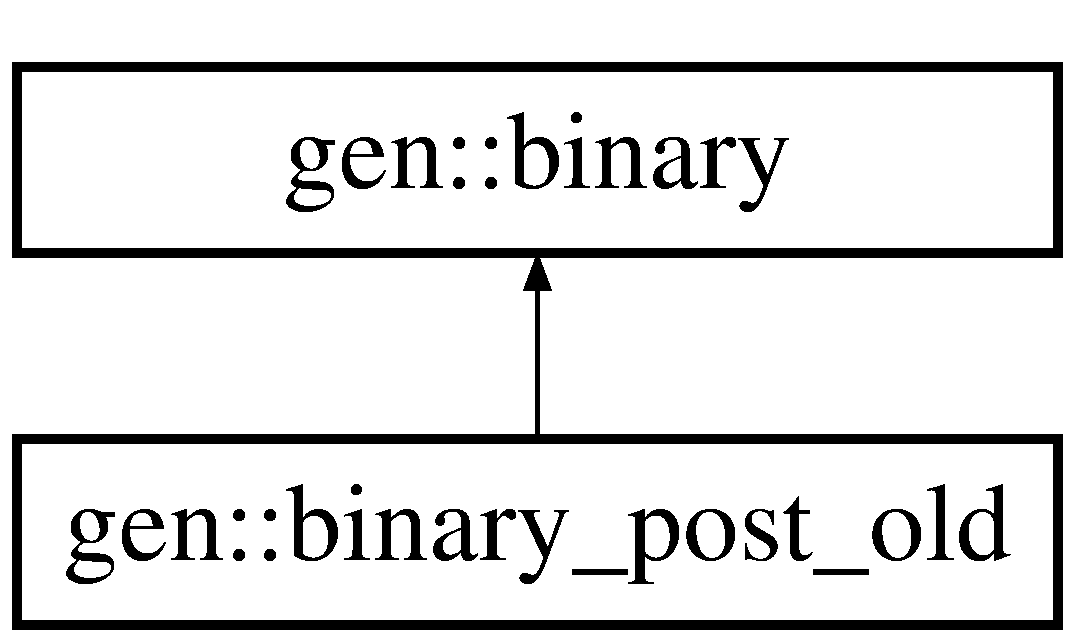
\includegraphics[height=2cm]{classgen_1_1binary__post__old}
\end{center}
\end{figure}
\subsection*{Public Member Functions}
\begin{CompactItemize}
\item 
def \hyperlink{classgen_1_1binary__post__old_17a34493ef0f01b2fdc3fb1f0cdf7c27}{\_\-\_\-init\_\-\_\-}
\begin{CompactList}\small\item\em Reads a dataset and construct the posterior probabilities of all linear models with variates regressed on target. \item\end{CompactList}\item 
def \hyperlink{classgen_1_1binary__post__old_4a2b39c9d4d59a01f64f0f593f5034c3}{lpmf}
\begin{CompactList}\small\item\em Evaluates the unnormalized log pmf. \item\end{CompactList}\item 
def \hyperlink{classgen_1_1binary__post__old_023a5d03ed9651fb97b76c933b23663d}{hb}
\begin{CompactList}\small\item\em Evaluates the log posterior density from a conjugate hierarchical setup (George, McCulloch, simplified). \item\end{CompactList}\item 
def \hyperlink{classgen_1_1binary__post__old_9ff0bcd17b79b57d04fa262c34074ac7}{bic}
\begin{CompactList}\small\item\em Evaluates the Bayesian Information Criterion. \item\end{CompactList}\item 
def \hyperlink{classgen_1_1binary__post__old_4529d5812825affd59fabf1d87879584}{explore}
\begin{CompactList}\small\item\em Explores the posterior for feasible dimensions. \item\end{CompactList}\end{CompactItemize}
\subsection*{Public Attributes}
\begin{CompactItemize}
\item 
\hyperlink{classgen_1_1binary__post__old_7f01b2229bc5804e960a1dc77bc6f846}{dataset}
\item 
\hyperlink{classgen_1_1binary__post__old_5293c3847ad6c37030d24d41b4a4eab2}{scoretype}
\item 
\hyperlink{classgen_1_1binary__post__old_2587b7ffadd5f860d7a3ab12756e95f3}{variates}
\item 
\hyperlink{classgen_1_1binary__post__old_9538d9a27640ca3c4f4a850f846f0d31}{target}
\item 
\hyperlink{classgen_1_1binary__post__old_216afb9d00f9463d7a5a903a40d20bf4}{n}
\item 
\hyperlink{classgen_1_1binary__post__old_926ce6ac7ef52ea4771dc948c1194b97}{p}
\item 
\hyperlink{classgen_1_1binary__post__old_3b3a31af2ddcba10547123ed91fc9d1f}{feasible}
\item 
\hyperlink{classgen_1_1binary__post__old_a2da390b89edbeba2f85014b6a2ac3ac}{X}
\item 
\hyperlink{classgen_1_1binary__post__old_2cf316c3b6750ee8f1a76bbda529e948}{Y}
\item 
\hyperlink{classgen_1_1binary__post__old_0c4ed9122532713d86b1c9f07c23ec2e}{names}
\item 
\hyperlink{classgen_1_1binary__post__old_80491b8bc4038ad90f318e951b7a09e9}{dim}
\item 
\hyperlink{classgen_1_1binary__post__old_1117a52fa6957e208fd5fcfd240e3fdb}{nozero}
\item 
\hyperlink{classgen_1_1binary__post__old_ba64762a3d525a8fc7d6722d8f0b3d79}{name}
\item 
\hyperlink{classgen_1_1binary__post__old_7e161b92c592af29da87881171431060}{title}
\item 
\hyperlink{classgen_1_1binary__post__old_de5ca8168e12417a339875aecde1b5e4}{XtY}
\item 
\hyperlink{classgen_1_1binary__post__old_e0c9510b59efacc1af2e8541ca814f59}{XtX}
\item 
\hyperlink{classgen_1_1binary__post__old_7adec8797994071a78edc8c5727336d3}{c1}
\item 
\hyperlink{classgen_1_1binary__post__old_10f35d33de2a393287d487c7a4362154}{c2}
\item 
\hyperlink{classgen_1_1binary__post__old_1cb800e469204fec167fc5429a228a2d}{c3}
\item 
\hyperlink{classgen_1_1binary__post__old_6510c634aa2f413c1a71e05be4b06de7}{loglevel}
\end{CompactItemize}
\subsection*{Private Member Functions}
\begin{CompactItemize}
\item 
def \hyperlink{classgen_1_1binary__post__old_8c38416d6a1e4cc27cc2c63f86328fb7}{\_\-pmf}
\begin{CompactList}\small\item\em Evaluates unnormalized pmf. \item\end{CompactList}\item 
def \hyperlink{classgen_1_1binary__post__old_8a67ce87638a15897ced3053c461e881}{\_\-rvs}
\begin{CompactList}\small\item\em Generates a sample from the posterior density rejecting from a proposals of p independent 0.5-binary variables. \item\end{CompactList}\end{CompactItemize}


\subsection{Member Function Documentation}
\hypertarget{classgen_1_1binary__post__old_17a34493ef0f01b2fdc3fb1f0cdf7c27}{
\index{gen::binary\_\-post\_\-old@{gen::binary\_\-post\_\-old}!\_\-\_\-init\_\-\_\-@{\_\-\_\-init\_\-\_\-}}
\index{\_\-\_\-init\_\-\_\-@{\_\-\_\-init\_\-\_\-}!gen::binary_post_old@{gen::binary\_\-post\_\-old}}
\subsubsection[{\_\-\_\-init\_\-\_\-}]{\setlength{\rightskip}{0pt plus 5cm}def gen::binary\_\-post\_\-old::\_\-\_\-init\_\-\_\- ( {\em self}, \/   {\em target}, \/   {\em variates}, \/   {\em dataset} = {\tt 'boston'}, \/   {\em scoretype} = {\tt 'hb'}, \/   {\em intercept} = {\tt True})}}
\label{classgen_1_1binary__post__old_17a34493ef0f01b2fdc3fb1f0cdf7c27}


Reads a dataset and construct the posterior probabilities of all linear models with variates regressed on target. 

target the column to regress on data vector of columns used as regressors \hypertarget{classgen_1_1binary__post__old_8c38416d6a1e4cc27cc2c63f86328fb7}{
\index{gen::binary\_\-post\_\-old@{gen::binary\_\-post\_\-old}!\_\-pmf@{\_\-pmf}}
\index{\_\-pmf@{\_\-pmf}!gen::binary_post_old@{gen::binary\_\-post\_\-old}}
\subsubsection[{\_\-pmf}]{\setlength{\rightskip}{0pt plus 5cm}def gen::binary\_\-post\_\-old::\_\-pmf ( {\em self}, \/   {\em gamma})\hspace{0.3cm}{\tt  \mbox{[}private\mbox{]}}}}
\label{classgen_1_1binary__post__old_8c38416d6a1e4cc27cc2c63f86328fb7}


Evaluates unnormalized pmf. 

gamma a \hyperlink{classgen_1_1binary}{binary} vector of length p \hypertarget{classgen_1_1binary__post__old_8a67ce87638a15897ced3053c461e881}{
\index{gen::binary\_\-post\_\-old@{gen::binary\_\-post\_\-old}!\_\-rvs@{\_\-rvs}}
\index{\_\-rvs@{\_\-rvs}!gen::binary_post_old@{gen::binary\_\-post\_\-old}}
\subsubsection[{\_\-rvs}]{\setlength{\rightskip}{0pt plus 5cm}def gen::binary\_\-post\_\-old::\_\-rvs ( {\em self})\hspace{0.3cm}{\tt  \mbox{[}private\mbox{]}}}}
\label{classgen_1_1binary__post__old_8a67ce87638a15897ced3053c461e881}


Generates a sample from the posterior density rejecting from a proposals of p independent 0.5-binary variables. 

If p $>$ MAX\_\-FEASIBLE the method returns a zero vector. \hypertarget{classgen_1_1binary__post__old_9ff0bcd17b79b57d04fa262c34074ac7}{
\index{gen::binary\_\-post\_\-old@{gen::binary\_\-post\_\-old}!bic@{bic}}
\index{bic@{bic}!gen::binary_post_old@{gen::binary\_\-post\_\-old}}
\subsubsection[{bic}]{\setlength{\rightskip}{0pt plus 5cm}def gen::binary\_\-post\_\-old::bic ( {\em self}, \/   {\em gamma})}}
\label{classgen_1_1binary__post__old_9ff0bcd17b79b57d04fa262c34074ac7}


Evaluates the Bayesian Information Criterion. 

gamma a \hyperlink{classgen_1_1binary}{binary} vector of length p \hypertarget{classgen_1_1binary__post__old_4529d5812825affd59fabf1d87879584}{
\index{gen::binary\_\-post\_\-old@{gen::binary\_\-post\_\-old}!explore@{explore}}
\index{explore@{explore}!gen::binary_post_old@{gen::binary\_\-post\_\-old}}
\subsubsection[{explore}]{\setlength{\rightskip}{0pt plus 5cm}def gen::binary\_\-post\_\-old::explore ( {\em self})}}
\label{classgen_1_1binary__post__old_4529d5812825affd59fabf1d87879584}


Explores the posterior for feasible dimensions. 

\hypertarget{classgen_1_1binary__post__old_023a5d03ed9651fb97b76c933b23663d}{
\index{gen::binary\_\-post\_\-old@{gen::binary\_\-post\_\-old}!hb@{hb}}
\index{hb@{hb}!gen::binary_post_old@{gen::binary\_\-post\_\-old}}
\subsubsection[{hb}]{\setlength{\rightskip}{0pt plus 5cm}def gen::binary\_\-post\_\-old::hb ( {\em self}, \/   {\em gamma})}}
\label{classgen_1_1binary__post__old_023a5d03ed9651fb97b76c933b23663d}


Evaluates the log posterior density from a conjugate hierarchical setup (George, McCulloch, simplified). 

gamma a \hyperlink{classgen_1_1binary}{binary} vector of length p \hypertarget{classgen_1_1binary__post__old_4a2b39c9d4d59a01f64f0f593f5034c3}{
\index{gen::binary\_\-post\_\-old@{gen::binary\_\-post\_\-old}!lpmf@{lpmf}}
\index{lpmf@{lpmf}!gen::binary_post_old@{gen::binary\_\-post\_\-old}}
\subsubsection[{lpmf}]{\setlength{\rightskip}{0pt plus 5cm}def gen::binary\_\-post\_\-old::lpmf ( {\em self}, \/   {\em gamma})}}
\label{classgen_1_1binary__post__old_4a2b39c9d4d59a01f64f0f593f5034c3}


Evaluates the unnormalized log pmf. 

gamma a \hyperlink{classgen_1_1binary}{binary} vector of length p 

Reimplemented from \hyperlink{classgen_1_1binary_0377b3ffdd44806d72453d0b8ead1758}{gen::binary}.

\subsection{Member Data Documentation}
\hypertarget{classgen_1_1binary__post__old_7adec8797994071a78edc8c5727336d3}{
\index{gen::binary\_\-post\_\-old@{gen::binary\_\-post\_\-old}!c1@{c1}}
\index{c1@{c1}!gen::binary_post_old@{gen::binary\_\-post\_\-old}}
\subsubsection[{c1}]{\setlength{\rightskip}{0pt plus 5cm}{\bf gen::binary\_\-post\_\-old::c1}}}
\label{classgen_1_1binary__post__old_7adec8797994071a78edc8c5727336d3}


\hypertarget{classgen_1_1binary__post__old_10f35d33de2a393287d487c7a4362154}{
\index{gen::binary\_\-post\_\-old@{gen::binary\_\-post\_\-old}!c2@{c2}}
\index{c2@{c2}!gen::binary_post_old@{gen::binary\_\-post\_\-old}}
\subsubsection[{c2}]{\setlength{\rightskip}{0pt plus 5cm}{\bf gen::binary\_\-post\_\-old::c2}}}
\label{classgen_1_1binary__post__old_10f35d33de2a393287d487c7a4362154}


\hypertarget{classgen_1_1binary__post__old_1cb800e469204fec167fc5429a228a2d}{
\index{gen::binary\_\-post\_\-old@{gen::binary\_\-post\_\-old}!c3@{c3}}
\index{c3@{c3}!gen::binary_post_old@{gen::binary\_\-post\_\-old}}
\subsubsection[{c3}]{\setlength{\rightskip}{0pt plus 5cm}{\bf gen::binary\_\-post\_\-old::c3}}}
\label{classgen_1_1binary__post__old_1cb800e469204fec167fc5429a228a2d}


\hypertarget{classgen_1_1binary__post__old_7f01b2229bc5804e960a1dc77bc6f846}{
\index{gen::binary\_\-post\_\-old@{gen::binary\_\-post\_\-old}!dataset@{dataset}}
\index{dataset@{dataset}!gen::binary_post_old@{gen::binary\_\-post\_\-old}}
\subsubsection[{dataset}]{\setlength{\rightskip}{0pt plus 5cm}{\bf gen::binary\_\-post\_\-old::dataset}}}
\label{classgen_1_1binary__post__old_7f01b2229bc5804e960a1dc77bc6f846}


\hypertarget{classgen_1_1binary__post__old_80491b8bc4038ad90f318e951b7a09e9}{
\index{gen::binary\_\-post\_\-old@{gen::binary\_\-post\_\-old}!dim@{dim}}
\index{dim@{dim}!gen::binary_post_old@{gen::binary\_\-post\_\-old}}
\subsubsection[{dim}]{\setlength{\rightskip}{0pt plus 5cm}{\bf gen::binary\_\-post\_\-old::dim}}}
\label{classgen_1_1binary__post__old_80491b8bc4038ad90f318e951b7a09e9}




Reimplemented from \hyperlink{classgen_1_1binary_37e0504e82a2e1117ed23ff2d8617274}{gen::binary}.\hypertarget{classgen_1_1binary__post__old_3b3a31af2ddcba10547123ed91fc9d1f}{
\index{gen::binary\_\-post\_\-old@{gen::binary\_\-post\_\-old}!feasible@{feasible}}
\index{feasible@{feasible}!gen::binary_post_old@{gen::binary\_\-post\_\-old}}
\subsubsection[{feasible}]{\setlength{\rightskip}{0pt plus 5cm}{\bf gen::binary\_\-post\_\-old::feasible}}}
\label{classgen_1_1binary__post__old_3b3a31af2ddcba10547123ed91fc9d1f}


\hypertarget{classgen_1_1binary__post__old_6510c634aa2f413c1a71e05be4b06de7}{
\index{gen::binary\_\-post\_\-old@{gen::binary\_\-post\_\-old}!loglevel@{loglevel}}
\index{loglevel@{loglevel}!gen::binary_post_old@{gen::binary\_\-post\_\-old}}
\subsubsection[{loglevel}]{\setlength{\rightskip}{0pt plus 5cm}{\bf gen::binary\_\-post\_\-old::loglevel}}}
\label{classgen_1_1binary__post__old_6510c634aa2f413c1a71e05be4b06de7}


\hypertarget{classgen_1_1binary__post__old_216afb9d00f9463d7a5a903a40d20bf4}{
\index{gen::binary\_\-post\_\-old@{gen::binary\_\-post\_\-old}!n@{n}}
\index{n@{n}!gen::binary_post_old@{gen::binary\_\-post\_\-old}}
\subsubsection[{n}]{\setlength{\rightskip}{0pt plus 5cm}{\bf gen::binary\_\-post\_\-old::n}}}
\label{classgen_1_1binary__post__old_216afb9d00f9463d7a5a903a40d20bf4}


\hypertarget{classgen_1_1binary__post__old_ba64762a3d525a8fc7d6722d8f0b3d79}{
\index{gen::binary\_\-post\_\-old@{gen::binary\_\-post\_\-old}!name@{name}}
\index{name@{name}!gen::binary_post_old@{gen::binary\_\-post\_\-old}}
\subsubsection[{name}]{\setlength{\rightskip}{0pt plus 5cm}{\bf gen::binary\_\-post\_\-old::name}}}
\label{classgen_1_1binary__post__old_ba64762a3d525a8fc7d6722d8f0b3d79}


\hypertarget{classgen_1_1binary__post__old_0c4ed9122532713d86b1c9f07c23ec2e}{
\index{gen::binary\_\-post\_\-old@{gen::binary\_\-post\_\-old}!names@{names}}
\index{names@{names}!gen::binary_post_old@{gen::binary\_\-post\_\-old}}
\subsubsection[{names}]{\setlength{\rightskip}{0pt plus 5cm}{\bf gen::binary\_\-post\_\-old::names}}}
\label{classgen_1_1binary__post__old_0c4ed9122532713d86b1c9f07c23ec2e}


\hypertarget{classgen_1_1binary__post__old_1117a52fa6957e208fd5fcfd240e3fdb}{
\index{gen::binary\_\-post\_\-old@{gen::binary\_\-post\_\-old}!nozero@{nozero}}
\index{nozero@{nozero}!gen::binary_post_old@{gen::binary\_\-post\_\-old}}
\subsubsection[{nozero}]{\setlength{\rightskip}{0pt plus 5cm}{\bf gen::binary\_\-post\_\-old::nozero}}}
\label{classgen_1_1binary__post__old_1117a52fa6957e208fd5fcfd240e3fdb}




Reimplemented from \hyperlink{classgen_1_1binary_ca500be68fab85fb9606fcb4c5be8f64}{gen::binary}.\hypertarget{classgen_1_1binary__post__old_926ce6ac7ef52ea4771dc948c1194b97}{
\index{gen::binary\_\-post\_\-old@{gen::binary\_\-post\_\-old}!p@{p}}
\index{p@{p}!gen::binary_post_old@{gen::binary\_\-post\_\-old}}
\subsubsection[{p}]{\setlength{\rightskip}{0pt plus 5cm}{\bf gen::binary\_\-post\_\-old::p}}}
\label{classgen_1_1binary__post__old_926ce6ac7ef52ea4771dc948c1194b97}




Reimplemented from \hyperlink{classgen_1_1binary_838502808c65c543b3cb558435047f92}{gen::binary}.\hypertarget{classgen_1_1binary__post__old_5293c3847ad6c37030d24d41b4a4eab2}{
\index{gen::binary\_\-post\_\-old@{gen::binary\_\-post\_\-old}!scoretype@{scoretype}}
\index{scoretype@{scoretype}!gen::binary_post_old@{gen::binary\_\-post\_\-old}}
\subsubsection[{scoretype}]{\setlength{\rightskip}{0pt plus 5cm}{\bf gen::binary\_\-post\_\-old::scoretype}}}
\label{classgen_1_1binary__post__old_5293c3847ad6c37030d24d41b4a4eab2}


\hypertarget{classgen_1_1binary__post__old_9538d9a27640ca3c4f4a850f846f0d31}{
\index{gen::binary\_\-post\_\-old@{gen::binary\_\-post\_\-old}!target@{target}}
\index{target@{target}!gen::binary_post_old@{gen::binary\_\-post\_\-old}}
\subsubsection[{target}]{\setlength{\rightskip}{0pt plus 5cm}{\bf gen::binary\_\-post\_\-old::target}}}
\label{classgen_1_1binary__post__old_9538d9a27640ca3c4f4a850f846f0d31}


\hypertarget{classgen_1_1binary__post__old_7e161b92c592af29da87881171431060}{
\index{gen::binary\_\-post\_\-old@{gen::binary\_\-post\_\-old}!title@{title}}
\index{title@{title}!gen::binary_post_old@{gen::binary\_\-post\_\-old}}
\subsubsection[{title}]{\setlength{\rightskip}{0pt plus 5cm}{\bf gen::binary\_\-post\_\-old::title}}}
\label{classgen_1_1binary__post__old_7e161b92c592af29da87881171431060}


\hypertarget{classgen_1_1binary__post__old_2587b7ffadd5f860d7a3ab12756e95f3}{
\index{gen::binary\_\-post\_\-old@{gen::binary\_\-post\_\-old}!variates@{variates}}
\index{variates@{variates}!gen::binary_post_old@{gen::binary\_\-post\_\-old}}
\subsubsection[{variates}]{\setlength{\rightskip}{0pt plus 5cm}{\bf gen::binary\_\-post\_\-old::variates}}}
\label{classgen_1_1binary__post__old_2587b7ffadd5f860d7a3ab12756e95f3}


\hypertarget{classgen_1_1binary__post__old_a2da390b89edbeba2f85014b6a2ac3ac}{
\index{gen::binary\_\-post\_\-old@{gen::binary\_\-post\_\-old}!X@{X}}
\index{X@{X}!gen::binary_post_old@{gen::binary\_\-post\_\-old}}
\subsubsection[{X}]{\setlength{\rightskip}{0pt plus 5cm}{\bf gen::binary\_\-post\_\-old::X}}}
\label{classgen_1_1binary__post__old_a2da390b89edbeba2f85014b6a2ac3ac}


\hypertarget{classgen_1_1binary__post__old_e0c9510b59efacc1af2e8541ca814f59}{
\index{gen::binary\_\-post\_\-old@{gen::binary\_\-post\_\-old}!XtX@{XtX}}
\index{XtX@{XtX}!gen::binary_post_old@{gen::binary\_\-post\_\-old}}
\subsubsection[{XtX}]{\setlength{\rightskip}{0pt plus 5cm}{\bf gen::binary\_\-post\_\-old::XtX}}}
\label{classgen_1_1binary__post__old_e0c9510b59efacc1af2e8541ca814f59}


\hypertarget{classgen_1_1binary__post__old_de5ca8168e12417a339875aecde1b5e4}{
\index{gen::binary\_\-post\_\-old@{gen::binary\_\-post\_\-old}!XtY@{XtY}}
\index{XtY@{XtY}!gen::binary_post_old@{gen::binary\_\-post\_\-old}}
\subsubsection[{XtY}]{\setlength{\rightskip}{0pt plus 5cm}{\bf gen::binary\_\-post\_\-old::XtY}}}
\label{classgen_1_1binary__post__old_de5ca8168e12417a339875aecde1b5e4}


\hypertarget{classgen_1_1binary__post__old_2cf316c3b6750ee8f1a76bbda529e948}{
\index{gen::binary\_\-post\_\-old@{gen::binary\_\-post\_\-old}!Y@{Y}}
\index{Y@{Y}!gen::binary_post_old@{gen::binary\_\-post\_\-old}}
\subsubsection[{Y}]{\setlength{\rightskip}{0pt plus 5cm}{\bf gen::binary\_\-post\_\-old::Y}}}
\label{classgen_1_1binary__post__old_2cf316c3b6750ee8f1a76bbda529e948}




The documentation for this class was generated from the following file:\begin{CompactItemize}
\item 
/mnt/eden/cschafer/Documents/smcdss/trunk/src/\hyperlink{gen_8py}{gen.py}\end{CompactItemize}

\hypertarget{classbvnorm_1_1bvnorm__gen}{
\section{bvnorm::bvnorm\_\-gen Class Reference}
\label{classbvnorm_1_1bvnorm__gen}\index{bvnorm::bvnorm\_\-gen@{bvnorm::bvnorm\_\-gen}}
}
\subsection*{Public Member Functions}
\begin{CompactItemize}
\item 
def \hyperlink{classbvnorm_1_1bvnorm__gen_628377c8e017c5314b8a5ef36db8d892}{cdf}
\begin{CompactList}\small\item\em Computes the bivariate normal cumulative distribution function, i.e. \item\end{CompactList}\item 
def \hyperlink{classbvnorm_1_1bvnorm__gen_e259683554c1efa1017f733f0824a38a}{pdf}
\begin{CompactList}\small\item\em Computes the bivariate normal probability distribution function, i.e. \item\end{CompactList}\item 
def \hyperlink{classbvnorm_1_1bvnorm__gen_eee6362a2e4206e66e79425e4f5431d5}{lowerDW}
\begin{CompactList}\small\item\em Computes bivariate normal probabilities; lowerDW calculates the probability that x $<$ dh and y $<$ dk using the Drezner-Wesolowsky approximation. \item\end{CompactList}\item 
def \hyperlink{classbvnorm_1_1bvnorm__gen_bd58b5d4090258a364bcb50619b24b08}{upperDW}
\begin{CompactList}\small\item\em Computes bivariate normal probabilities; upperDW calculates the probability that x $>$ dh and y $>$ dk. \item\end{CompactList}\item 
def \hyperlink{classbvnorm_1_1bvnorm__gen_00b5b765f63ca54c859717b98744d9dc}{lowerDI}
\begin{CompactList}\small\item\em Computes bivariate normal probabilities; lowerDW calculates the probability that x $<$ dh and y $<$ dk using the Drezner-Wesolowsky approximation. \item\end{CompactList}\item 
def \hyperlink{classbvnorm_1_1bvnorm__gen_a21b04c4ce48d3215ead047576149238}{upperDI}
\begin{CompactList}\small\item\em Computes bivariate normal probabilities; upperDW calculates the probability that x $>$ dh and y $>$ dk. \item\end{CompactList}\item 
def \hyperlink{classbvnorm_1_1bvnorm__gen_86b9c8b6b258da3a7eb66cd91b00416b}{lowerMC}
\begin{CompactList}\small\item\em Computes bivariate normal probabilities; lowerMC calculates the probability that x $<$ dh and y $<$ dk using a Monte Carlo approximation of n samples. \item\end{CompactList}\item 
def \hyperlink{classbvnorm_1_1bvnorm__gen_65e19caa62c397d0e2de0e4d66a57d26}{upperMC}
\begin{CompactList}\small\item\em Computes bivariate normal probabilities; upperMC calculates the probability that x $>$ dh and y $>$ dk. \item\end{CompactList}\end{CompactItemize}
\subsection*{Private Member Functions}
\begin{CompactItemize}
\item 
def \hyperlink{classbvnorm_1_1bvnorm__gen_1f85ab2898c7ce352de4eaa9b47d6817}{\_\-rvs}
\item 
def \hyperlink{classbvnorm_1_1bvnorm__gen_5c395f39255b5b08cc050672e0094ca5}{\_\-\_\-W}
\begin{CompactList}\small\item\em Auxiliary function for Divgi method. \item\end{CompactList}\end{CompactItemize}


\subsection{Member Function Documentation}
\hypertarget{classbvnorm_1_1bvnorm__gen_5c395f39255b5b08cc050672e0094ca5}{
\index{bvnorm::bvnorm\_\-gen@{bvnorm::bvnorm\_\-gen}!\_\-\_\-W@{\_\-\_\-W}}
\index{\_\-\_\-W@{\_\-\_\-W}!bvnorm::bvnorm_gen@{bvnorm::bvnorm\_\-gen}}
\subsubsection[{\_\-\_\-W}]{\setlength{\rightskip}{0pt plus 5cm}def bvnorm::bvnorm\_\-gen::\_\-\_\-W ( {\em R}, \/   {\em psi})\hspace{0.3cm}{\tt  \mbox{[}private\mbox{]}}}}
\label{classbvnorm_1_1bvnorm__gen_5c395f39255b5b08cc050672e0094ca5}


Auxiliary function for Divgi method. 

\hypertarget{classbvnorm_1_1bvnorm__gen_1f85ab2898c7ce352de4eaa9b47d6817}{
\index{bvnorm::bvnorm\_\-gen@{bvnorm::bvnorm\_\-gen}!\_\-rvs@{\_\-rvs}}
\index{\_\-rvs@{\_\-rvs}!bvnorm::bvnorm_gen@{bvnorm::bvnorm\_\-gen}}
\subsubsection[{\_\-rvs}]{\setlength{\rightskip}{0pt plus 5cm}def bvnorm::bvnorm\_\-gen::\_\-rvs ( {\em self}, \/   {\em r} = {\tt 0})\hspace{0.3cm}{\tt  \mbox{[}private\mbox{]}}}}
\label{classbvnorm_1_1bvnorm__gen_1f85ab2898c7ce352de4eaa9b47d6817}


\hypertarget{classbvnorm_1_1bvnorm__gen_628377c8e017c5314b8a5ef36db8d892}{
\index{bvnorm::bvnorm\_\-gen@{bvnorm::bvnorm\_\-gen}!cdf@{cdf}}
\index{cdf@{cdf}!bvnorm::bvnorm_gen@{bvnorm::bvnorm\_\-gen}}
\subsubsection[{cdf}]{\setlength{\rightskip}{0pt plus 5cm}def bvnorm::bvnorm\_\-gen::cdf ( {\em self}, \/   {\em x}, \/   {\em r} = {\tt 0})}}
\label{classbvnorm_1_1bvnorm__gen_628377c8e017c5314b8a5ef36db8d892}


Computes the bivariate normal cumulative distribution function, i.e. 

the probability that X $<$ x and Y $<$ y.

The function only calls lowerDW(x, y, r). \hypertarget{classbvnorm_1_1bvnorm__gen_00b5b765f63ca54c859717b98744d9dc}{
\index{bvnorm::bvnorm\_\-gen@{bvnorm::bvnorm\_\-gen}!lowerDI@{lowerDI}}
\index{lowerDI@{lowerDI}!bvnorm::bvnorm_gen@{bvnorm::bvnorm\_\-gen}}
\subsubsection[{lowerDI}]{\setlength{\rightskip}{0pt plus 5cm}def bvnorm::bvnorm\_\-gen::lowerDI ( {\em dh}, \/   {\em dk}, \/   {\em r})}}
\label{classbvnorm_1_1bvnorm__gen_00b5b765f63ca54c859717b98744d9dc}


Computes bivariate normal probabilities; lowerDW calculates the probability that x $<$ dh and y $<$ dk using the Drezner-Wesolowsky approximation. 

The function only calls upperDI(-dh, -dk, r). \hypertarget{classbvnorm_1_1bvnorm__gen_eee6362a2e4206e66e79425e4f5431d5}{
\index{bvnorm::bvnorm\_\-gen@{bvnorm::bvnorm\_\-gen}!lowerDW@{lowerDW}}
\index{lowerDW@{lowerDW}!bvnorm::bvnorm_gen@{bvnorm::bvnorm\_\-gen}}
\subsubsection[{lowerDW}]{\setlength{\rightskip}{0pt plus 5cm}def bvnorm::bvnorm\_\-gen::lowerDW ( {\em self}, \/   {\em dh}, \/   {\em dk}, \/   {\em r})}}
\label{classbvnorm_1_1bvnorm__gen_eee6362a2e4206e66e79425e4f5431d5}


Computes bivariate normal probabilities; lowerDW calculates the probability that x $<$ dh and y $<$ dk using the Drezner-Wesolowsky approximation. 

The function only calls upperDW(-dh, -dk, r). \hypertarget{classbvnorm_1_1bvnorm__gen_86b9c8b6b258da3a7eb66cd91b00416b}{
\index{bvnorm::bvnorm\_\-gen@{bvnorm::bvnorm\_\-gen}!lowerMC@{lowerMC}}
\index{lowerMC@{lowerMC}!bvnorm::bvnorm_gen@{bvnorm::bvnorm\_\-gen}}
\subsubsection[{lowerMC}]{\setlength{\rightskip}{0pt plus 5cm}def bvnorm::bvnorm\_\-gen::lowerMC ( {\em self}, \/   {\em dh}, \/   {\em dk}, \/   {\em r}, \/   {\em n} = {\tt 100000})}}
\label{classbvnorm_1_1bvnorm__gen_86b9c8b6b258da3a7eb66cd91b00416b}


Computes bivariate normal probabilities; lowerMC calculates the probability that x $<$ dh and y $<$ dk using a Monte Carlo approximation of n samples. 

The function only calls upperMC(-dh, -dk, r, n). \hypertarget{classbvnorm_1_1bvnorm__gen_e259683554c1efa1017f733f0824a38a}{
\index{bvnorm::bvnorm\_\-gen@{bvnorm::bvnorm\_\-gen}!pdf@{pdf}}
\index{pdf@{pdf}!bvnorm::bvnorm_gen@{bvnorm::bvnorm\_\-gen}}
\subsubsection[{pdf}]{\setlength{\rightskip}{0pt plus 5cm}def bvnorm::bvnorm\_\-gen::pdf ( {\em self}, \/   {\em x}, \/   {\em r} = {\tt 0})}}
\label{classbvnorm_1_1bvnorm__gen_e259683554c1efa1017f733f0824a38a}


Computes the bivariate normal probability distribution function, i.e. 

the density at (x, y) \hypertarget{classbvnorm_1_1bvnorm__gen_a21b04c4ce48d3215ead047576149238}{
\index{bvnorm::bvnorm\_\-gen@{bvnorm::bvnorm\_\-gen}!upperDI@{upperDI}}
\index{upperDI@{upperDI}!bvnorm::bvnorm_gen@{bvnorm::bvnorm\_\-gen}}
\subsubsection[{upperDI}]{\setlength{\rightskip}{0pt plus 5cm}def bvnorm::bvnorm\_\-gen::upperDI ( {\em dh}, \/   {\em dk}, \/   {\em r})}}
\label{classbvnorm_1_1bvnorm__gen_a21b04c4ce48d3215ead047576149238}


Computes bivariate normal probabilities; upperDW calculates the probability that x $>$ dh and y $>$ dk. 

dh 1st lower integration limit dk 2nd lower integration limit r correlation coefficient

This function is based on the method described by D.R. Divgi, (1979), \char`\"{}Calculation of univariate and bivariate normal probability functions\char`\"{}, Teh Annals of Statistics, Vol.7, No.4, pp. 903-910.

The function does not yet deliver the correct values for every correlation coefficient r. \hypertarget{classbvnorm_1_1bvnorm__gen_bd58b5d4090258a364bcb50619b24b08}{
\index{bvnorm::bvnorm\_\-gen@{bvnorm::bvnorm\_\-gen}!upperDW@{upperDW}}
\index{upperDW@{upperDW}!bvnorm::bvnorm_gen@{bvnorm::bvnorm\_\-gen}}
\subsubsection[{upperDW}]{\setlength{\rightskip}{0pt plus 5cm}def bvnorm::bvnorm\_\-gen::upperDW ( {\em self}, \/   {\em dh}, \/   {\em dk}, \/   {\em r})}}
\label{classbvnorm_1_1bvnorm__gen_bd58b5d4090258a364bcb50619b24b08}


Computes bivariate normal probabilities; upperDW calculates the probability that x $>$ dh and y $>$ dk. 

dh 1st lower integration limit dk 2nd lower integration limit r correlation coefficient

This function is based on the method described by Z. Drezner and G.O. Wesolowsky, (1989), \char`\"{}On the computation of the bivariate normal integral\char`\"{}, Journal of Statist. Comput. Simul. 35, pp. 101-107, with major modifications for double precision, for $|$r$|$ close to 1.

The code was adapted for python from the matlab routine by Alan Genz. \hypertarget{classbvnorm_1_1bvnorm__gen_65e19caa62c397d0e2de0e4d66a57d26}{
\index{bvnorm::bvnorm\_\-gen@{bvnorm::bvnorm\_\-gen}!upperMC@{upperMC}}
\index{upperMC@{upperMC}!bvnorm::bvnorm_gen@{bvnorm::bvnorm\_\-gen}}
\subsubsection[{upperMC}]{\setlength{\rightskip}{0pt plus 5cm}def bvnorm::bvnorm\_\-gen::upperMC ( {\em self}, \/   {\em dh}, \/   {\em dk}, \/   {\em r}, \/   {\em n} = {\tt 100000})}}
\label{classbvnorm_1_1bvnorm__gen_65e19caa62c397d0e2de0e4d66a57d26}


Computes bivariate normal probabilities; upperMC calculates the probability that x $>$ dh and y $>$ dk. 

dh 1st lower integration limit dk 2nd lower integration limit r correlation coefficient n sample size (=100000)

This function is a simple MC evaluation used to cross-check the approximation algorithms DW and DI. 

The documentation for this class was generated from the following file:\begin{CompactItemize}
\item 
/mnt/eden/cschafer/Documents/smcdss/trunk/src/\hyperlink{bvnorm_8py}{bvnorm.py}\end{CompactItemize}

\hypertarget{classsampling_1_1data}{
\section{sampling::data Class Reference}
\label{classsampling_1_1data}\index{sampling::data@{sampling::data}}
}
\subsection*{Public Member Functions}
\begin{CompactItemize}
\item 
def \hyperlink{classsampling_1_1data_c53c5f40743a4e9972bbea4814133163}{\_\-\_\-init\_\-\_\-}
\begin{CompactList}\small\item\em The \hyperlink{classsampling_1_1data}{data} class holds a list of random samples. \item\end{CompactList}\item 
def \hyperlink{classsampling_1_1data_9276fda7f43c819a4bc405dafba8cb90}{append}
\item 
def \hyperlink{classsampling_1_1data_7e4d9b676ac16687825f8698511904e4}{toarray}
\item 
def \hyperlink{classsampling_1_1data_ca31acb9a3f5ac73c6b578560f1d85c3}{tolist}
\item 
def \hyperlink{classsampling_1_1data_6b0070f25fb05379d9ab4847e6d7d7ca}{data}
\item 
def \hyperlink{classsampling_1_1data_e59799438bbe2136d082d67e95a84afd}{weights}
\item 
def \hyperlink{classsampling_1_1data_c5d34a6d4c38963e9f61fca1fdfb214f}{clear}
\item 
def \hyperlink{classsampling_1_1data_e25008002e4e7869ec5047bf6b6bba36}{size}
\item 
def \hyperlink{classsampling_1_1data_91e88ff11c431b763c1b073fc10ef9cc}{dim}
\item 
def \hyperlink{classsampling_1_1data_036c155076bf9069de078c8fb8102336}{cov}
\item 
def \hyperlink{classsampling_1_1data_0c7353cefc1e45a887f5341455afc3d8}{cor}
\item 
def \hyperlink{classsampling_1_1data_043fedd9515c040a518b9f1571af5e40}{mean}
\item 
def \hyperlink{classsampling_1_1data_ffd8218cbffd08dd6a5943e50dce29fb}{setweights}
\item 
def \hyperlink{classsampling_1_1data_55bd6270b85c5a80aa4a74b0fd2b44cb}{sort}
\item 
def \hyperlink{classsampling_1_1data_97ca284cf4c50daa748273be76f0d18b}{shrink}
\item 
def \hyperlink{classsampling_1_1data_a2b26e86169aedbf74e2f86e24a7b1db}{copy}
\end{CompactItemize}
\subsection*{Public Attributes}
\begin{CompactItemize}
\item 
\hyperlink{classsampling_1_1data_160aaf82abdd3a24d5a830dc1b0ed378}{dataset}
\item 
\hyperlink{classsampling_1_1data_837dbe448267fb2e235d6a398b196d54}{weightset}
\item 
\hyperlink{classsampling_1_1data_223cf6ee3aba8358113a5102faa2a0a4}{isArray}
\item 
\hyperlink{classsampling_1_1data_2ab52d0cab7a32cef923f0669a1c8bdc}{nweightset}
\item 
\hyperlink{classsampling_1_1data_eda6d7c1dcf0af8f69404e3bdc72c324}{order}
\item 
\hyperlink{classsampling_1_1data_59d39eb206fcc37334749abc5f223b89}{index}
\end{CompactItemize}


\subsection{Constructor \& Destructor Documentation}
\hypertarget{classsampling_1_1data_6b0070f25fb05379d9ab4847e6d7d7ca}{
\index{sampling::data@{sampling::data}!data@{data}}
\index{data@{data}!sampling::data@{sampling::data}}
\subsubsection[{data}]{\setlength{\rightskip}{0pt plus 5cm}def sampling::data::data ( {\em self}, \/   {\em ordered} = {\tt False}, \/   {\em fraction} = {\tt 1}, \/   {\em dtype} = {\tt int})}}
\label{classsampling_1_1data_6b0070f25fb05379d9ab4847e6d7d7ca}




\subsection{Member Function Documentation}
\hypertarget{classsampling_1_1data_c53c5f40743a4e9972bbea4814133163}{
\index{sampling::data@{sampling::data}!\_\-\_\-init\_\-\_\-@{\_\-\_\-init\_\-\_\-}}
\index{\_\-\_\-init\_\-\_\-@{\_\-\_\-init\_\-\_\-}!sampling::data@{sampling::data}}
\subsubsection[{\_\-\_\-init\_\-\_\-}]{\setlength{\rightskip}{0pt plus 5cm}def sampling::data::\_\-\_\-init\_\-\_\- ( {\em self}, \/   {\em dataset} = {\tt None}, \/   {\em index} = {\tt None}, \/   {\em weightset} = {\tt None})}}
\label{classsampling_1_1data_c53c5f40743a4e9972bbea4814133163}


The \hyperlink{classsampling_1_1data}{data} class holds a list of random samples. 

\hypertarget{classsampling_1_1data_9276fda7f43c819a4bc405dafba8cb90}{
\index{sampling::data@{sampling::data}!append@{append}}
\index{append@{append}!sampling::data@{sampling::data}}
\subsubsection[{append}]{\setlength{\rightskip}{0pt plus 5cm}def sampling::data::append ( {\em self}, \/   {\em sample}, \/   {\em weight} = {\tt None})}}
\label{classsampling_1_1data_9276fda7f43c819a4bc405dafba8cb90}


\hypertarget{classsampling_1_1data_c5d34a6d4c38963e9f61fca1fdfb214f}{
\index{sampling::data@{sampling::data}!clear@{clear}}
\index{clear@{clear}!sampling::data@{sampling::data}}
\subsubsection[{clear}]{\setlength{\rightskip}{0pt plus 5cm}def sampling::data::clear ( {\em self}, \/   {\em fraction} = {\tt 1})}}
\label{classsampling_1_1data_c5d34a6d4c38963e9f61fca1fdfb214f}


\hypertarget{classsampling_1_1data_a2b26e86169aedbf74e2f86e24a7b1db}{
\index{sampling::data@{sampling::data}!copy@{copy}}
\index{copy@{copy}!sampling::data@{sampling::data}}
\subsubsection[{copy}]{\setlength{\rightskip}{0pt plus 5cm}def sampling::data::copy ( {\em self})}}
\label{classsampling_1_1data_a2b26e86169aedbf74e2f86e24a7b1db}


\hypertarget{classsampling_1_1data_0c7353cefc1e45a887f5341455afc3d8}{
\index{sampling::data@{sampling::data}!cor@{cor}}
\index{cor@{cor}!sampling::data@{sampling::data}}
\subsubsection[{cor}]{\setlength{\rightskip}{0pt plus 5cm}def sampling::data::cor ( {\em self}, \/   {\em weighted} = {\tt False}, \/   {\em fraction} = {\tt 1})}}
\label{classsampling_1_1data_0c7353cefc1e45a887f5341455afc3d8}


\hypertarget{classsampling_1_1data_036c155076bf9069de078c8fb8102336}{
\index{sampling::data@{sampling::data}!cov@{cov}}
\index{cov@{cov}!sampling::data@{sampling::data}}
\subsubsection[{cov}]{\setlength{\rightskip}{0pt plus 5cm}def sampling::data::cov ( {\em self}, \/   {\em weighted} = {\tt False}, \/   {\em indexed} = {\tt False}, \/   {\em fraction} = {\tt 1})}}
\label{classsampling_1_1data_036c155076bf9069de078c8fb8102336}


\hypertarget{classsampling_1_1data_91e88ff11c431b763c1b073fc10ef9cc}{
\index{sampling::data@{sampling::data}!dim@{dim}}
\index{dim@{dim}!sampling::data@{sampling::data}}
\subsubsection[{dim}]{\setlength{\rightskip}{0pt plus 5cm}def sampling::data::dim ( {\em self})}}
\label{classsampling_1_1data_91e88ff11c431b763c1b073fc10ef9cc}


\hypertarget{classsampling_1_1data_043fedd9515c040a518b9f1571af5e40}{
\index{sampling::data@{sampling::data}!mean@{mean}}
\index{mean@{mean}!sampling::data@{sampling::data}}
\subsubsection[{mean}]{\setlength{\rightskip}{0pt plus 5cm}def sampling::data::mean ( {\em self}, \/   {\em weighted} = {\tt False}, \/   {\em indexed} = {\tt False}, \/   {\em fraction} = {\tt 1}, \/   {\em dtype} = {\tt int})}}
\label{classsampling_1_1data_043fedd9515c040a518b9f1571af5e40}


\hypertarget{classsampling_1_1data_ffd8218cbffd08dd6a5943e50dce29fb}{
\index{sampling::data@{sampling::data}!setweights@{setweights}}
\index{setweights@{setweights}!sampling::data@{sampling::data}}
\subsubsection[{setweights}]{\setlength{\rightskip}{0pt plus 5cm}def sampling::data::setweights ( {\em self}, \/   {\em post})}}
\label{classsampling_1_1data_ffd8218cbffd08dd6a5943e50dce29fb}


\hypertarget{classsampling_1_1data_97ca284cf4c50daa748273be76f0d18b}{
\index{sampling::data@{sampling::data}!shrink@{shrink}}
\index{shrink@{shrink}!sampling::data@{sampling::data}}
\subsubsection[{shrink}]{\setlength{\rightskip}{0pt plus 5cm}def sampling::data::shrink ( {\em self}, \/   {\em index})}}
\label{classsampling_1_1data_97ca284cf4c50daa748273be76f0d18b}


\hypertarget{classsampling_1_1data_e25008002e4e7869ec5047bf6b6bba36}{
\index{sampling::data@{sampling::data}!size@{size}}
\index{size@{size}!sampling::data@{sampling::data}}
\subsubsection[{size}]{\setlength{\rightskip}{0pt plus 5cm}def sampling::data::size ( {\em self})}}
\label{classsampling_1_1data_e25008002e4e7869ec5047bf6b6bba36}


\hypertarget{classsampling_1_1data_55bd6270b85c5a80aa4a74b0fd2b44cb}{
\index{sampling::data@{sampling::data}!sort@{sort}}
\index{sort@{sort}!sampling::data@{sampling::data}}
\subsubsection[{sort}]{\setlength{\rightskip}{0pt plus 5cm}def sampling::data::sort ( {\em self})}}
\label{classsampling_1_1data_55bd6270b85c5a80aa4a74b0fd2b44cb}


\hypertarget{classsampling_1_1data_7e4d9b676ac16687825f8698511904e4}{
\index{sampling::data@{sampling::data}!toarray@{toarray}}
\index{toarray@{toarray}!sampling::data@{sampling::data}}
\subsubsection[{toarray}]{\setlength{\rightskip}{0pt plus 5cm}def sampling::data::toarray ( {\em self})}}
\label{classsampling_1_1data_7e4d9b676ac16687825f8698511904e4}


\hypertarget{classsampling_1_1data_ca31acb9a3f5ac73c6b578560f1d85c3}{
\index{sampling::data@{sampling::data}!tolist@{tolist}}
\index{tolist@{tolist}!sampling::data@{sampling::data}}
\subsubsection[{tolist}]{\setlength{\rightskip}{0pt plus 5cm}def sampling::data::tolist ( {\em self})}}
\label{classsampling_1_1data_ca31acb9a3f5ac73c6b578560f1d85c3}


\hypertarget{classsampling_1_1data_e59799438bbe2136d082d67e95a84afd}{
\index{sampling::data@{sampling::data}!weights@{weights}}
\index{weights@{weights}!sampling::data@{sampling::data}}
\subsubsection[{weights}]{\setlength{\rightskip}{0pt plus 5cm}def sampling::data::weights ( {\em self}, \/   {\em ordered} = {\tt False}, \/   {\em fraction} = {\tt 1})}}
\label{classsampling_1_1data_e59799438bbe2136d082d67e95a84afd}




\subsection{Member Data Documentation}
\hypertarget{classsampling_1_1data_160aaf82abdd3a24d5a830dc1b0ed378}{
\index{sampling::data@{sampling::data}!dataset@{dataset}}
\index{dataset@{dataset}!sampling::data@{sampling::data}}
\subsubsection[{dataset}]{\setlength{\rightskip}{0pt plus 5cm}{\bf sampling::data::dataset}}}
\label{classsampling_1_1data_160aaf82abdd3a24d5a830dc1b0ed378}


\hypertarget{classsampling_1_1data_59d39eb206fcc37334749abc5f223b89}{
\index{sampling::data@{sampling::data}!index@{index}}
\index{index@{index}!sampling::data@{sampling::data}}
\subsubsection[{index}]{\setlength{\rightskip}{0pt plus 5cm}{\bf sampling::data::index}}}
\label{classsampling_1_1data_59d39eb206fcc37334749abc5f223b89}


\hypertarget{classsampling_1_1data_223cf6ee3aba8358113a5102faa2a0a4}{
\index{sampling::data@{sampling::data}!isArray@{isArray}}
\index{isArray@{isArray}!sampling::data@{sampling::data}}
\subsubsection[{isArray}]{\setlength{\rightskip}{0pt plus 5cm}{\bf sampling::data::isArray}}}
\label{classsampling_1_1data_223cf6ee3aba8358113a5102faa2a0a4}


\hypertarget{classsampling_1_1data_2ab52d0cab7a32cef923f0669a1c8bdc}{
\index{sampling::data@{sampling::data}!nweightset@{nweightset}}
\index{nweightset@{nweightset}!sampling::data@{sampling::data}}
\subsubsection[{nweightset}]{\setlength{\rightskip}{0pt plus 5cm}{\bf sampling::data::nweightset}}}
\label{classsampling_1_1data_2ab52d0cab7a32cef923f0669a1c8bdc}


\hypertarget{classsampling_1_1data_eda6d7c1dcf0af8f69404e3bdc72c324}{
\index{sampling::data@{sampling::data}!order@{order}}
\index{order@{order}!sampling::data@{sampling::data}}
\subsubsection[{order}]{\setlength{\rightskip}{0pt plus 5cm}{\bf sampling::data::order}}}
\label{classsampling_1_1data_eda6d7c1dcf0af8f69404e3bdc72c324}


\hypertarget{classsampling_1_1data_837dbe448267fb2e235d6a398b196d54}{
\index{sampling::data@{sampling::data}!weightset@{weightset}}
\index{weightset@{weightset}!sampling::data@{sampling::data}}
\subsubsection[{weightset}]{\setlength{\rightskip}{0pt plus 5cm}{\bf sampling::data::weightset}}}
\label{classsampling_1_1data_837dbe448267fb2e235d6a398b196d54}




The documentation for this class was generated from the following file:\begin{CompactItemize}
\item 
/mnt/eden/cschafer/Documents/smcdss/trunk/src/\hyperlink{sampling_8py}{sampling.py}\end{CompactItemize}

\hypertarget{classmcmc_1_1mcmc}{
\section{mcmc::mcmc Class Reference}
\label{classmcmc_1_1mcmc}\index{mcmc::mcmc@{mcmc::mcmc}}
}
\subsection*{Public Member Functions}
\begin{CompactItemize}
\item 
def \hyperlink{classmcmc_1_1mcmc_0a65f27f35aa71a335bc5e5b633b5242}{domcmc}
\begin{CompactList}\small\item\em Runs a MCMC \hyperlink{namespacesampling}{sampling} scheme to approximate the marginal distribution. \item\end{CompactList}\item 
def \hyperlink{classmcmc_1_1mcmc_54669cdc319c8ef04f8030a1b2b3664e}{kernel\_\-gibbs}
\item 
def \hyperlink{classmcmc_1_1mcmc_d42bf6f27a081b18507d87576cfa00e7}{kernel\_\-indmh}
\item 
def \hyperlink{classmcmc_1_1mcmc_92084a28766545a03bc2b45c0e858a99}{printMarginalProbs}
\item 
def \hyperlink{classmcmc_1_1mcmc_61ddda03459f328c4190dd15041909a9}{plotSteps}
\end{CompactItemize}
\subsection*{Public Attributes}
\begin{CompactItemize}
\item 
\hyperlink{classmcmc_1_1mcmc_b775e315b3afd728337a7ce76e051757}{verbose}
\item 
\hyperlink{classmcmc_1_1mcmc_3ae6df3dc0f30424737f9553e4ccdd59}{plot}
\item 
\hyperlink{classmcmc_1_1mcmc_75cf003947dd468b37dbe3db7c3be77b}{targetDistr}
\item 
\hyperlink{classmcmc_1_1mcmc_595bfdf51ae7ecb2ddb4c0729e134f31}{score}
\item 
\hyperlink{classmcmc_1_1mcmc_c0da164af953d15a6e59005616b78581}{kernel}
\item 
\hyperlink{classmcmc_1_1mcmc_76f97dc69cc27fe654f700e7612f2ace}{scaleneighbors}
\item 
\hyperlink{classmcmc_1_1mcmc_cd47deafd7039aa45fefd45af5db9a7c}{maxval}
\item 
\hyperlink{classmcmc_1_1mcmc_d44a8fd5b0a9d827b6922f9829a20fdf}{state\_\-change}
\item 
\hyperlink{classmcmc_1_1mcmc_e2b88838a2868340e27b6467368c16d7}{pdata}
\end{CompactItemize}


\subsection{Member Function Documentation}
\hypertarget{classmcmc_1_1mcmc_0a65f27f35aa71a335bc5e5b633b5242}{
\index{mcmc::mcmc@{mcmc::mcmc}!domcmc@{domcmc}}
\index{domcmc@{domcmc}!mcmc::mcmc@{mcmc::mcmc}}
\subsubsection[{domcmc}]{\setlength{\rightskip}{0pt plus 5cm}def mcmc::mcmc::domcmc ( {\em self}, \/   {\em targetDistr} = {\tt None}, \/   {\em maxtime} = {\tt inf}, \/   {\em ths\_\-iter} = {\tt inf}, \/   {\em verbose} = {\tt False}, \/   {\em kernel} = {\tt 'mh'}, \/   {\em singlestep} = {\tt 10000}, \/   {\em plot} = {\tt False})}}
\label{classmcmc_1_1mcmc_0a65f27f35aa71a335bc5e5b633b5242}


Runs a MCMC \hyperlink{namespacesampling}{sampling} scheme to approximate the marginal distribution. 

\hypertarget{classmcmc_1_1mcmc_54669cdc319c8ef04f8030a1b2b3664e}{
\index{mcmc::mcmc@{mcmc::mcmc}!kernel\_\-gibbs@{kernel\_\-gibbs}}
\index{kernel\_\-gibbs@{kernel\_\-gibbs}!mcmc::mcmc@{mcmc::mcmc}}
\subsubsection[{kernel\_\-gibbs}]{\setlength{\rightskip}{0pt plus 5cm}def mcmc::mcmc::kernel\_\-gibbs ( {\em self}, \/   {\em state})}}
\label{classmcmc_1_1mcmc_54669cdc319c8ef04f8030a1b2b3664e}


\hypertarget{classmcmc_1_1mcmc_d42bf6f27a081b18507d87576cfa00e7}{
\index{mcmc::mcmc@{mcmc::mcmc}!kernel\_\-indmh@{kernel\_\-indmh}}
\index{kernel\_\-indmh@{kernel\_\-indmh}!mcmc::mcmc@{mcmc::mcmc}}
\subsubsection[{kernel\_\-indmh}]{\setlength{\rightskip}{0pt plus 5cm}def mcmc::mcmc::kernel\_\-indmh ( {\em self}, \/   {\em state})}}
\label{classmcmc_1_1mcmc_d42bf6f27a081b18507d87576cfa00e7}


\hypertarget{classmcmc_1_1mcmc_61ddda03459f328c4190dd15041909a9}{
\index{mcmc::mcmc@{mcmc::mcmc}!plotSteps@{plotSteps}}
\index{plotSteps@{plotSteps}!mcmc::mcmc@{mcmc::mcmc}}
\subsubsection[{plotSteps}]{\setlength{\rightskip}{0pt plus 5cm}def mcmc::mcmc::plotSteps ( {\em self}, \/   {\em step})}}
\label{classmcmc_1_1mcmc_61ddda03459f328c4190dd15041909a9}


\hypertarget{classmcmc_1_1mcmc_92084a28766545a03bc2b45c0e858a99}{
\index{mcmc::mcmc@{mcmc::mcmc}!printMarginalProbs@{printMarginalProbs}}
\index{printMarginalProbs@{printMarginalProbs}!mcmc::mcmc@{mcmc::mcmc}}
\subsubsection[{printMarginalProbs}]{\setlength{\rightskip}{0pt plus 5cm}def mcmc::mcmc::printMarginalProbs ( {\em self})}}
\label{classmcmc_1_1mcmc_92084a28766545a03bc2b45c0e858a99}




\subsection{Member Data Documentation}
\hypertarget{classmcmc_1_1mcmc_c0da164af953d15a6e59005616b78581}{
\index{mcmc::mcmc@{mcmc::mcmc}!kernel@{kernel}}
\index{kernel@{kernel}!mcmc::mcmc@{mcmc::mcmc}}
\subsubsection[{kernel}]{\setlength{\rightskip}{0pt plus 5cm}{\bf mcmc::mcmc::kernel}}}
\label{classmcmc_1_1mcmc_c0da164af953d15a6e59005616b78581}


\hypertarget{classmcmc_1_1mcmc_cd47deafd7039aa45fefd45af5db9a7c}{
\index{mcmc::mcmc@{mcmc::mcmc}!maxval@{maxval}}
\index{maxval@{maxval}!mcmc::mcmc@{mcmc::mcmc}}
\subsubsection[{maxval}]{\setlength{\rightskip}{0pt plus 5cm}{\bf mcmc::mcmc::maxval}}}
\label{classmcmc_1_1mcmc_cd47deafd7039aa45fefd45af5db9a7c}


\hypertarget{classmcmc_1_1mcmc_e2b88838a2868340e27b6467368c16d7}{
\index{mcmc::mcmc@{mcmc::mcmc}!pdata@{pdata}}
\index{pdata@{pdata}!mcmc::mcmc@{mcmc::mcmc}}
\subsubsection[{pdata}]{\setlength{\rightskip}{0pt plus 5cm}{\bf mcmc::mcmc::pdata}}}
\label{classmcmc_1_1mcmc_e2b88838a2868340e27b6467368c16d7}


\hypertarget{classmcmc_1_1mcmc_3ae6df3dc0f30424737f9553e4ccdd59}{
\index{mcmc::mcmc@{mcmc::mcmc}!plot@{plot}}
\index{plot@{plot}!mcmc::mcmc@{mcmc::mcmc}}
\subsubsection[{plot}]{\setlength{\rightskip}{0pt plus 5cm}{\bf mcmc::mcmc::plot}}}
\label{classmcmc_1_1mcmc_3ae6df3dc0f30424737f9553e4ccdd59}


\hypertarget{classmcmc_1_1mcmc_76f97dc69cc27fe654f700e7612f2ace}{
\index{mcmc::mcmc@{mcmc::mcmc}!scaleneighbors@{scaleneighbors}}
\index{scaleneighbors@{scaleneighbors}!mcmc::mcmc@{mcmc::mcmc}}
\subsubsection[{scaleneighbors}]{\setlength{\rightskip}{0pt plus 5cm}{\bf mcmc::mcmc::scaleneighbors}}}
\label{classmcmc_1_1mcmc_76f97dc69cc27fe654f700e7612f2ace}


\hypertarget{classmcmc_1_1mcmc_595bfdf51ae7ecb2ddb4c0729e134f31}{
\index{mcmc::mcmc@{mcmc::mcmc}!score@{score}}
\index{score@{score}!mcmc::mcmc@{mcmc::mcmc}}
\subsubsection[{score}]{\setlength{\rightskip}{0pt plus 5cm}{\bf mcmc::mcmc::score}}}
\label{classmcmc_1_1mcmc_595bfdf51ae7ecb2ddb4c0729e134f31}


\hypertarget{classmcmc_1_1mcmc_d44a8fd5b0a9d827b6922f9829a20fdf}{
\index{mcmc::mcmc@{mcmc::mcmc}!state\_\-change@{state\_\-change}}
\index{state\_\-change@{state\_\-change}!mcmc::mcmc@{mcmc::mcmc}}
\subsubsection[{state\_\-change}]{\setlength{\rightskip}{0pt plus 5cm}{\bf mcmc::mcmc::state\_\-change}}}
\label{classmcmc_1_1mcmc_d44a8fd5b0a9d827b6922f9829a20fdf}


\hypertarget{classmcmc_1_1mcmc_75cf003947dd468b37dbe3db7c3be77b}{
\index{mcmc::mcmc@{mcmc::mcmc}!targetDistr@{targetDistr}}
\index{targetDistr@{targetDistr}!mcmc::mcmc@{mcmc::mcmc}}
\subsubsection[{targetDistr}]{\setlength{\rightskip}{0pt plus 5cm}{\bf mcmc::mcmc::targetDistr}}}
\label{classmcmc_1_1mcmc_75cf003947dd468b37dbe3db7c3be77b}


\hypertarget{classmcmc_1_1mcmc_b775e315b3afd728337a7ce76e051757}{
\index{mcmc::mcmc@{mcmc::mcmc}!verbose@{verbose}}
\index{verbose@{verbose}!mcmc::mcmc@{mcmc::mcmc}}
\subsubsection[{verbose}]{\setlength{\rightskip}{0pt plus 5cm}{\bf mcmc::mcmc::verbose}}}
\label{classmcmc_1_1mcmc_b775e315b3afd728337a7ce76e051757}




The documentation for this class was generated from the following file:\begin{CompactItemize}
\item 
/mnt/eden/cschafer/Documents/smcdss/trunk/src/\hyperlink{mcmc_8py}{mcmc.py}\end{CompactItemize}

\hypertarget{classsampling_1_1sampler}{
\section{sampling::sampler Class Reference}
\label{classsampling_1_1sampler}\index{sampling::sampler@{sampling::sampler}}
}
\subsection*{Public Member Functions}
\begin{CompactItemize}
\item 
def \hyperlink{classsampling_1_1sampler_1f14a8e3d0700779dcdac79def1c33d3}{\_\-\_\-init\_\-\_\-}
\begin{CompactList}\small\item\em The \hyperlink{classsampling_1_1sampler}{sampler} class holds a \hyperlink{classsampling_1_1data}{data} object and fills it with random samples from a given generator. \item\end{CompactList}\item 
def \hyperlink{classsampling_1_1sampler_a3908666fdfd325eb00c171a267fe650}{sample}
\end{CompactItemize}
\subsection*{Public Attributes}
\begin{CompactItemize}
\item 
\hyperlink{classsampling_1_1sampler_96f11b07709c74778ddd41e8d7ea1439}{gen}
\item 
\hyperlink{classsampling_1_1sampler_ac2f0763c7a907e0968b96b6e440ab5a}{data}
\item 
\hyperlink{classsampling_1_1sampler_5a11056b435de5e46629d6517120bb98}{targetDistr}
\end{CompactItemize}


\subsection{Member Function Documentation}
\hypertarget{classsampling_1_1sampler_1f14a8e3d0700779dcdac79def1c33d3}{
\index{sampling::sampler@{sampling::sampler}!\_\-\_\-init\_\-\_\-@{\_\-\_\-init\_\-\_\-}}
\index{\_\-\_\-init\_\-\_\-@{\_\-\_\-init\_\-\_\-}!sampling::sampler@{sampling::sampler}}
\subsubsection[{\_\-\_\-init\_\-\_\-}]{\setlength{\rightskip}{0pt plus 5cm}def sampling::sampler::\_\-\_\-init\_\-\_\- ( {\em self}, \/   {\em gen}, \/   {\em targetDistr} = {\tt None})}}
\label{classsampling_1_1sampler_1f14a8e3d0700779dcdac79def1c33d3}


The \hyperlink{classsampling_1_1sampler}{sampler} class holds a \hyperlink{classsampling_1_1data}{data} object and fills it with random samples from a given generator. 

generator a random number generator \hypertarget{classsampling_1_1sampler_a3908666fdfd325eb00c171a267fe650}{
\index{sampling::sampler@{sampling::sampler}!sample@{sample}}
\index{sample@{sample}!sampling::sampler@{sampling::sampler}}
\subsubsection[{sample}]{\setlength{\rightskip}{0pt plus 5cm}def sampling::sampler::sample ( {\em self}, \/   {\em size}, \/   {\em verbose} = {\tt False}, \/   {\em online} = {\tt False})}}
\label{classsampling_1_1sampler_a3908666fdfd325eb00c171a267fe650}




\subsection{Member Data Documentation}
\hypertarget{classsampling_1_1sampler_ac2f0763c7a907e0968b96b6e440ab5a}{
\index{sampling::sampler@{sampling::sampler}!data@{data}}
\index{data@{data}!sampling::sampler@{sampling::sampler}}
\subsubsection[{data}]{\setlength{\rightskip}{0pt plus 5cm}{\bf sampling::sampler::data}}}
\label{classsampling_1_1sampler_ac2f0763c7a907e0968b96b6e440ab5a}


\hypertarget{classsampling_1_1sampler_96f11b07709c74778ddd41e8d7ea1439}{
\index{sampling::sampler@{sampling::sampler}!gen@{gen}}
\index{gen@{gen}!sampling::sampler@{sampling::sampler}}
\subsubsection[{gen}]{\setlength{\rightskip}{0pt plus 5cm}{\bf sampling::sampler::gen}}}
\label{classsampling_1_1sampler_96f11b07709c74778ddd41e8d7ea1439}


\hypertarget{classsampling_1_1sampler_5a11056b435de5e46629d6517120bb98}{
\index{sampling::sampler@{sampling::sampler}!targetDistr@{targetDistr}}
\index{targetDistr@{targetDistr}!sampling::sampler@{sampling::sampler}}
\subsubsection[{targetDistr}]{\setlength{\rightskip}{0pt plus 5cm}{\bf sampling::sampler::targetDistr}}}
\label{classsampling_1_1sampler_5a11056b435de5e46629d6517120bb98}




The documentation for this class was generated from the following file:\begin{CompactItemize}
\item 
/mnt/eden/cschafer/Documents/smcdss/trunk/src/\hyperlink{sampling_8py}{sampling.py}\end{CompactItemize}

\hypertarget{classsmc_1_1smc}{
\section{smc::smc Class Reference}
\label{classsmc_1_1smc}\index{smc::smc@{smc::smc}}
}
Sequential Monte Carlo class for model choice problems.  


\subsection*{Public Member Functions}
\begin{CompactItemize}
\item 
def \hyperlink{classsmc_1_1smc_32f2ee107cd254620e678aac22a45d21}{dosmc}
\begin{CompactList}\small\item\em Construct a particle approximation to the target via sequential Monte Carlo methods. \item\end{CompactList}\item 
def \hyperlink{classsmc_1_1smc_e7f644f3b5cb36aa99f0ebf7b4ebc3a4}{estimatePriorDistr}
\begin{CompactList}\small\item\em Run a pilot Markov chain to estimate the prior distribution and the log level. \item\end{CompactList}\item 
def \hyperlink{classsmc_1_1smc_f567f3fc9711a87297d72cab09fea035}{estimateProposalDistr}
\begin{CompactList}\small\item\em Estimate the parameters of the proposal distribution from the particle system. \item\end{CompactList}\item 
def \hyperlink{classsmc_1_1smc_cf375f96d980adede8438b3fead19938}{moveParticleSystem}
\begin{CompactList}\small\item\em Move particles according to an MH kernel to fight depletion of the particle system. \item\end{CompactList}\item 
def \hyperlink{classsmc_1_1smc_747f9eabdfcb52a9a2ccf6ec84bfdb83}{kernel\_\-indmh}
\begin{CompactList}\small\item\em Metropolis Hasting kernel with independent proposal distribution estimated from the particle system. \item\end{CompactList}\item 
def \hyperlink{classsmc_1_1smc_698a2598642ff7f48f0b6ab87b0e81cc}{updateLogWeights}
\begin{CompactList}\small\item\em Update the log weights. \item\end{CompactList}\item 
def \hyperlink{classsmc_1_1smc_495a950f5dc0aa66fdf5279ae8ca6242}{normalize}
\begin{CompactList}\small\item\em Return normalized importance weights. \item\end{CompactList}\item 
def \hyperlink{classsmc_1_1smc_95aec6accabbea27d33eb8a5a4eb7ed2}{ess}
\begin{CompactList}\small\item\em Return effective sample size 1/(sum\_\-\{w  weights\} w$^\wedge$2) . \item\end{CompactList}\item 
def \hyperlink{classsmc_1_1smc_61bd1b39ab3f3dcbfe19cca533276937}{getParticleDiversity}
\begin{CompactList}\small\item\em Return the particle diversity. \item\end{CompactList}\item 
def \hyperlink{classsmc_1_1smc_7c417c930e9039fd1bbda56d40ceb38d}{resampleParticleSystem}
\begin{CompactList}\small\item\em Resample the particle system. \item\end{CompactList}\item 
def \hyperlink{classsmc_1_1smc_50453b83eb4dc3519a2be7cba5ae51c7}{logprior}
\begin{CompactList}\small\item\em Return the prior log probability. \item\end{CompactList}\item 
def \hyperlink{classsmc_1_1smc_7af51336a53e7096b370af78e42e9cfa}{resample\_\-python}
\begin{CompactList}\small\item\em Compute the particle indices by residual resampling - adopted from Pierre's code. \item\end{CompactList}\item 
def \hyperlink{classsmc_1_1smc_75f94a2618bc58ed2cc419dc36817ff9}{resample\_\-weave}
\begin{CompactList}\small\item\em Compute the particle indices by residual resampling using scypy.weave. \item\end{CompactList}\item 
def \hyperlink{classsmc_1_1smc_462f5030ead3c90a3d7be5419a0539b6}{plotSteps}
\begin{CompactList}\small\item\em Plot the marginal probabilities and correlation matrix of the particle system. \item\end{CompactList}\item 
def \hyperlink{classsmc_1_1smc_485fc39676c507c373e922a124f51748}{printParticleStructure}
\begin{CompactList}\small\item\em Print out a summary of how many particles are n-fold in the particle system. \item\end{CompactList}\end{CompactItemize}
\subsection*{Public Attributes}
\begin{CompactItemize}
\item 
\hyperlink{classsmc_1_1smc_e3829faa0fc80c586754db6ff6be0e21}{plot}
\item 
\hyperlink{classsmc_1_1smc_38c24613680356068405f403b837c4c5}{verbose}
\item 
\hyperlink{classsmc_1_1smc_c63ef54a10ca8d071ccb44851861074d}{kappa}
\item 
\hyperlink{classsmc_1_1smc_30edcc21d770d259d6985d4b79c6d95d}{targetDistr}
\item 
\hyperlink{classsmc_1_1smc_927a6dd0b643bac0c5cadf396389b44d}{changeProposalDistr}
\item 
\hyperlink{classsmc_1_1smc_6162e817e2c67350cc277006bdb05b31}{rho}
\item 
\hyperlink{classsmc_1_1smc_44b55c368632379dd23476a13ff2c7e5}{n}
\item 
\hyperlink{classsmc_1_1smc_6487e2a8d1dd4e355f689c0a6ef2ddae}{ps}
\item 
\hyperlink{classsmc_1_1smc_0478d6b05231542beed9a2aa7c7cf1b6}{t}
\item 
\hyperlink{classsmc_1_1smc_21babd9a1ec1e969dd9ae3cc62c6dd1d}{loglevel}
\item 
\hyperlink{classsmc_1_1smc_55ec911b9b714e1103220453efe648be}{proposalDistr}
\item 
\hyperlink{classsmc_1_1smc_09b83207e06db24e39c512371d100485}{priorDistr}
\item 
\hyperlink{classsmc_1_1smc_1ee6881c16f30b39c30b365d3aeeb5f1}{pdata}
\end{CompactItemize}


\subsection{Detailed Description}
Sequential Monte Carlo class for model choice problems. 

\subsection{Member Function Documentation}
\hypertarget{classsmc_1_1smc_32f2ee107cd254620e678aac22a45d21}{
\index{smc::smc@{smc::smc}!dosmc@{dosmc}}
\index{dosmc@{dosmc}!smc::smc@{smc::smc}}
\subsubsection[{dosmc}]{\setlength{\rightskip}{0pt plus 5cm}def smc::smc::dosmc ( {\em self}, \/   {\em targetDistr}, \/   {\em nparticles}, \/   {\em kappa}, \/   {\em verbose} = {\tt True}, \/   {\em nbridge} = {\tt None}, \/   {\em plot} = {\tt False})}}
\label{classsmc_1_1smc_32f2ee107cd254620e678aac22a45d21}


Construct a particle approximation to the target via sequential Monte Carlo methods. 

\begin{Desc}
\item[Parameters:]
\begin{description}
\item[{\em targetDistr}]The target distribution. \item[{\em proposalDistr}]The proposal distributions. \item[{\em nbridge}]Number of bridge steps between the prior and the target. \item[{\em nparticles}]Number of particles. \item[{\em kappa}]Prior smoothing parameter: 0 $<$= kappa $<$= 1. \item[{\em plot}]True, if the steps are to be plotted. \item[{\em verbose}]True, if reports to standard are desired. \end{description}
\end{Desc}
\hypertarget{classsmc_1_1smc_95aec6accabbea27d33eb8a5a4eb7ed2}{
\index{smc::smc@{smc::smc}!ess@{ess}}
\index{ess@{ess}!smc::smc@{smc::smc}}
\subsubsection[{ess}]{\setlength{\rightskip}{0pt plus 5cm}def smc::smc::ess ( {\em self})}}
\label{classsmc_1_1smc_95aec6accabbea27d33eb8a5a4eb7ed2}


Return effective sample size 1/(sum\_\-\{w  weights\} w$^\wedge$2) . 

\hypertarget{classsmc_1_1smc_e7f644f3b5cb36aa99f0ebf7b4ebc3a4}{
\index{smc::smc@{smc::smc}!estimatePriorDistr@{estimatePriorDistr}}
\index{estimatePriorDistr@{estimatePriorDistr}!smc::smc@{smc::smc}}
\subsubsection[{estimatePriorDistr}]{\setlength{\rightskip}{0pt plus 5cm}def smc::smc::estimatePriorDistr ( {\em self}, \/   {\em steps})}}
\label{classsmc_1_1smc_e7f644f3b5cb36aa99f0ebf7b4ebc3a4}


Run a pilot Markov chain to estimate the prior distribution and the log level. 

\begin{Desc}
\item[Parameters:]
\begin{description}
\item[{\em steps}]Number of MCMC steps for the pilot run. \end{description}
\end{Desc}
\hypertarget{classsmc_1_1smc_f567f3fc9711a87297d72cab09fea035}{
\index{smc::smc@{smc::smc}!estimateProposalDistr@{estimateProposalDistr}}
\index{estimateProposalDistr@{estimateProposalDistr}!smc::smc@{smc::smc}}
\subsubsection[{estimateProposalDistr}]{\setlength{\rightskip}{0pt plus 5cm}def smc::smc::estimateProposalDistr ( {\em self})}}
\label{classsmc_1_1smc_f567f3fc9711a87297d72cab09fea035}


Estimate the parameters of the proposal distribution from the particle system. 

\hypertarget{classsmc_1_1smc_61bd1b39ab3f3dcbfe19cca533276937}{
\index{smc::smc@{smc::smc}!getParticleDiversity@{getParticleDiversity}}
\index{getParticleDiversity@{getParticleDiversity}!smc::smc@{smc::smc}}
\subsubsection[{getParticleDiversity}]{\setlength{\rightskip}{0pt plus 5cm}def smc::smc::getParticleDiversity ( {\em self})}}
\label{classsmc_1_1smc_61bd1b39ab3f3dcbfe19cca533276937}


Return the particle diversity. 

\hypertarget{classsmc_1_1smc_747f9eabdfcb52a9a2ccf6ec84bfdb83}{
\index{smc::smc@{smc::smc}!kernel\_\-indmh@{kernel\_\-indmh}}
\index{kernel\_\-indmh@{kernel\_\-indmh}!smc::smc@{smc::smc}}
\subsubsection[{kernel\_\-indmh}]{\setlength{\rightskip}{0pt plus 5cm}def smc::smc::kernel\_\-indmh ( {\em self}, \/   {\em index})}}
\label{classsmc_1_1smc_747f9eabdfcb52a9a2ccf6ec84bfdb83}


Metropolis Hasting kernel with independent proposal distribution estimated from the particle system. 

\begin{Desc}
\item[Parameters:]
\begin{description}
\item[{\em index}]Index of the particle to be processed by the kernel. \end{description}
\end{Desc}
\hypertarget{classsmc_1_1smc_50453b83eb4dc3519a2be7cba5ae51c7}{
\index{smc::smc@{smc::smc}!logprior@{logprior}}
\index{logprior@{logprior}!smc::smc@{smc::smc}}
\subsubsection[{logprior}]{\setlength{\rightskip}{0pt plus 5cm}def smc::smc::logprior ( {\em self}, \/   {\em x} = {\tt None})}}
\label{classsmc_1_1smc_50453b83eb4dc3519a2be7cba5ae51c7}


Return the prior log probability. 

\begin{Desc}
\item[Parameters:]
\begin{description}
\item[{\em x}]If x is an index, the function returns self.ps\mbox{[}'logprior'\mbox{]}\mbox{[}x\mbox{]} plus the log level. If x is a float, it returns x plus the log level. If x is not specified, it returns the vector self.ps\mbox{[}'logprior'\mbox{]} plus the loglevel. \end{description}
\end{Desc}
\hypertarget{classsmc_1_1smc_cf375f96d980adede8438b3fead19938}{
\index{smc::smc@{smc::smc}!moveParticleSystem@{moveParticleSystem}}
\index{moveParticleSystem@{moveParticleSystem}!smc::smc@{smc::smc}}
\subsubsection[{moveParticleSystem}]{\setlength{\rightskip}{0pt plus 5cm}def smc::smc::moveParticleSystem ( {\em self})}}
\label{classsmc_1_1smc_cf375f96d980adede8438b3fead19938}


Move particles according to an MH kernel to fight depletion of the particle system. 

\hypertarget{classsmc_1_1smc_495a950f5dc0aa66fdf5279ae8ca6242}{
\index{smc::smc@{smc::smc}!normalize@{normalize}}
\index{normalize@{normalize}!smc::smc@{smc::smc}}
\subsubsection[{normalize}]{\setlength{\rightskip}{0pt plus 5cm}def smc::smc::normalize ( {\em self})}}
\label{classsmc_1_1smc_495a950f5dc0aa66fdf5279ae8ca6242}


Return normalized importance weights. 

\hypertarget{classsmc_1_1smc_462f5030ead3c90a3d7be5419a0539b6}{
\index{smc::smc@{smc::smc}!plotSteps@{plotSteps}}
\index{plotSteps@{plotSteps}!smc::smc@{smc::smc}}
\subsubsection[{plotSteps}]{\setlength{\rightskip}{0pt plus 5cm}def smc::smc::plotSteps ( {\em self}, \/   {\em step})}}
\label{classsmc_1_1smc_462f5030ead3c90a3d7be5419a0539b6}


Plot the marginal probabilities and correlation matrix of the particle system. 

\hypertarget{classsmc_1_1smc_485fc39676c507c373e922a124f51748}{
\index{smc::smc@{smc::smc}!printParticleStructure@{printParticleStructure}}
\index{printParticleStructure@{printParticleStructure}!smc::smc@{smc::smc}}
\subsubsection[{printParticleStructure}]{\setlength{\rightskip}{0pt plus 5cm}def smc::smc::printParticleStructure ( {\em self})}}
\label{classsmc_1_1smc_485fc39676c507c373e922a124f51748}


Print out a summary of how many particles are n-fold in the particle system. 

\hypertarget{classsmc_1_1smc_7af51336a53e7096b370af78e42e9cfa}{
\index{smc::smc@{smc::smc}!resample\_\-python@{resample\_\-python}}
\index{resample\_\-python@{resample\_\-python}!smc::smc@{smc::smc}}
\subsubsection[{resample\_\-python}]{\setlength{\rightskip}{0pt plus 5cm}def smc::smc::resample\_\-python ( {\em self})}}
\label{classsmc_1_1smc_7af51336a53e7096b370af78e42e9cfa}


Compute the particle indices by residual resampling - adopted from Pierre's code. 

\hypertarget{classsmc_1_1smc_75f94a2618bc58ed2cc419dc36817ff9}{
\index{smc::smc@{smc::smc}!resample\_\-weave@{resample\_\-weave}}
\index{resample\_\-weave@{resample\_\-weave}!smc::smc@{smc::smc}}
\subsubsection[{resample\_\-weave}]{\setlength{\rightskip}{0pt plus 5cm}def smc::smc::resample\_\-weave ( {\em self})}}
\label{classsmc_1_1smc_75f94a2618bc58ed2cc419dc36817ff9}


Compute the particle indices by residual resampling using scypy.weave. 

\hypertarget{classsmc_1_1smc_7c417c930e9039fd1bbda56d40ceb38d}{
\index{smc::smc@{smc::smc}!resampleParticleSystem@{resampleParticleSystem}}
\index{resampleParticleSystem@{resampleParticleSystem}!smc::smc@{smc::smc}}
\subsubsection[{resampleParticleSystem}]{\setlength{\rightskip}{0pt plus 5cm}def smc::smc::resampleParticleSystem ( {\em self})}}
\label{classsmc_1_1smc_7c417c930e9039fd1bbda56d40ceb38d}


Resample the particle system. 

\hypertarget{classsmc_1_1smc_698a2598642ff7f48f0b6ab87b0e81cc}{
\index{smc::smc@{smc::smc}!updateLogWeights@{updateLogWeights}}
\index{updateLogWeights@{updateLogWeights}!smc::smc@{smc::smc}}
\subsubsection[{updateLogWeights}]{\setlength{\rightskip}{0pt plus 5cm}def smc::smc::updateLogWeights ( {\em self})}}
\label{classsmc_1_1smc_698a2598642ff7f48f0b6ab87b0e81cc}


Update the log weights. 

Return effective sample size. 

\subsection{Member Data Documentation}
\hypertarget{classsmc_1_1smc_927a6dd0b643bac0c5cadf396389b44d}{
\index{smc::smc@{smc::smc}!changeProposalDistr@{changeProposalDistr}}
\index{changeProposalDistr@{changeProposalDistr}!smc::smc@{smc::smc}}
\subsubsection[{changeProposalDistr}]{\setlength{\rightskip}{0pt plus 5cm}{\bf smc::smc::changeProposalDistr}}}
\label{classsmc_1_1smc_927a6dd0b643bac0c5cadf396389b44d}


\hypertarget{classsmc_1_1smc_c63ef54a10ca8d071ccb44851861074d}{
\index{smc::smc@{smc::smc}!kappa@{kappa}}
\index{kappa@{kappa}!smc::smc@{smc::smc}}
\subsubsection[{kappa}]{\setlength{\rightskip}{0pt plus 5cm}{\bf smc::smc::kappa}}}
\label{classsmc_1_1smc_c63ef54a10ca8d071ccb44851861074d}


\hypertarget{classsmc_1_1smc_21babd9a1ec1e969dd9ae3cc62c6dd1d}{
\index{smc::smc@{smc::smc}!loglevel@{loglevel}}
\index{loglevel@{loglevel}!smc::smc@{smc::smc}}
\subsubsection[{loglevel}]{\setlength{\rightskip}{0pt plus 5cm}{\bf smc::smc::loglevel}}}
\label{classsmc_1_1smc_21babd9a1ec1e969dd9ae3cc62c6dd1d}


\hypertarget{classsmc_1_1smc_44b55c368632379dd23476a13ff2c7e5}{
\index{smc::smc@{smc::smc}!n@{n}}
\index{n@{n}!smc::smc@{smc::smc}}
\subsubsection[{n}]{\setlength{\rightskip}{0pt plus 5cm}{\bf smc::smc::n}}}
\label{classsmc_1_1smc_44b55c368632379dd23476a13ff2c7e5}


\hypertarget{classsmc_1_1smc_1ee6881c16f30b39c30b365d3aeeb5f1}{
\index{smc::smc@{smc::smc}!pdata@{pdata}}
\index{pdata@{pdata}!smc::smc@{smc::smc}}
\subsubsection[{pdata}]{\setlength{\rightskip}{0pt plus 5cm}{\bf smc::smc::pdata}}}
\label{classsmc_1_1smc_1ee6881c16f30b39c30b365d3aeeb5f1}


\hypertarget{classsmc_1_1smc_e3829faa0fc80c586754db6ff6be0e21}{
\index{smc::smc@{smc::smc}!plot@{plot}}
\index{plot@{plot}!smc::smc@{smc::smc}}
\subsubsection[{plot}]{\setlength{\rightskip}{0pt plus 5cm}{\bf smc::smc::plot}}}
\label{classsmc_1_1smc_e3829faa0fc80c586754db6ff6be0e21}


\hypertarget{classsmc_1_1smc_09b83207e06db24e39c512371d100485}{
\index{smc::smc@{smc::smc}!priorDistr@{priorDistr}}
\index{priorDistr@{priorDistr}!smc::smc@{smc::smc}}
\subsubsection[{priorDistr}]{\setlength{\rightskip}{0pt plus 5cm}{\bf smc::smc::priorDistr}}}
\label{classsmc_1_1smc_09b83207e06db24e39c512371d100485}


\hypertarget{classsmc_1_1smc_55ec911b9b714e1103220453efe648be}{
\index{smc::smc@{smc::smc}!proposalDistr@{proposalDistr}}
\index{proposalDistr@{proposalDistr}!smc::smc@{smc::smc}}
\subsubsection[{proposalDistr}]{\setlength{\rightskip}{0pt plus 5cm}{\bf smc::smc::proposalDistr}}}
\label{classsmc_1_1smc_55ec911b9b714e1103220453efe648be}


\hypertarget{classsmc_1_1smc_6487e2a8d1dd4e355f689c0a6ef2ddae}{
\index{smc::smc@{smc::smc}!ps@{ps}}
\index{ps@{ps}!smc::smc@{smc::smc}}
\subsubsection[{ps}]{\setlength{\rightskip}{0pt plus 5cm}{\bf smc::smc::ps}}}
\label{classsmc_1_1smc_6487e2a8d1dd4e355f689c0a6ef2ddae}


\hypertarget{classsmc_1_1smc_6162e817e2c67350cc277006bdb05b31}{
\index{smc::smc@{smc::smc}!rho@{rho}}
\index{rho@{rho}!smc::smc@{smc::smc}}
\subsubsection[{rho}]{\setlength{\rightskip}{0pt plus 5cm}{\bf smc::smc::rho}}}
\label{classsmc_1_1smc_6162e817e2c67350cc277006bdb05b31}


\hypertarget{classsmc_1_1smc_0478d6b05231542beed9a2aa7c7cf1b6}{
\index{smc::smc@{smc::smc}!t@{t}}
\index{t@{t}!smc::smc@{smc::smc}}
\subsubsection[{t}]{\setlength{\rightskip}{0pt plus 5cm}{\bf smc::smc::t}}}
\label{classsmc_1_1smc_0478d6b05231542beed9a2aa7c7cf1b6}


\hypertarget{classsmc_1_1smc_30edcc21d770d259d6985d4b79c6d95d}{
\index{smc::smc@{smc::smc}!targetDistr@{targetDistr}}
\index{targetDistr@{targetDistr}!smc::smc@{smc::smc}}
\subsubsection[{targetDistr}]{\setlength{\rightskip}{0pt plus 5cm}{\bf smc::smc::targetDistr}}}
\label{classsmc_1_1smc_30edcc21d770d259d6985d4b79c6d95d}


\hypertarget{classsmc_1_1smc_38c24613680356068405f403b837c4c5}{
\index{smc::smc@{smc::smc}!verbose@{verbose}}
\index{verbose@{verbose}!smc::smc@{smc::smc}}
\subsubsection[{verbose}]{\setlength{\rightskip}{0pt plus 5cm}{\bf smc::smc::verbose}}}
\label{classsmc_1_1smc_38c24613680356068405f403b837c4c5}




The documentation for this class was generated from the following file:\begin{CompactItemize}
\item 
/mnt/eden/cschafer/Documents/smcdss/trunk/src/\hyperlink{smc_8py}{smc.py}\end{CompactItemize}

\chapter{File Documentation}
\hypertarget{bvnorm_8py}{
\section{/mnt/eden/cschafer/Documents/smcdss/trunk/src/bvnorm.py File Reference}
\label{bvnorm_8py}\index{/mnt/eden/cschafer/Documents/smcdss/trunk/src/bvnorm.py@{/mnt/eden/cschafer/Documents/smcdss/trunk/src/bvnorm.py}}
}
\subsection*{Classes}
\begin{CompactItemize}
\item 
class \hyperlink{classbvnorm_1_1bvnorm__gen}{bvnorm::bvnorm\_\-gen}
\end{CompactItemize}
\subsection*{Namespaces}
\begin{CompactItemize}
\item 
namespace \hyperlink{namespacebvnorm}{bvnorm}
\end{CompactItemize}
\subsection*{Variables}
\begin{CompactItemize}
\item 
tuple \hyperlink{namespacebvnorm_ffd1e4833c9d3af70673f92d0e9bb471}{bvnorm::bvnorm} = bvnorm\_\-gen(name='bvnorm', longname='A bivariate normal', shapes='r', extradoc=\char`\"{}\char`\"{}\char`\"{}Bivariate normal distribution with correlation r.normal.pdf(x,y) = exp(-(x$\ast$x-2$\ast$r$\ast$x$\ast$y+y$\ast$y)/(2$\ast$(1-r$\ast$r))) / (2$\ast$pi$\ast$sqrt(1-r$\ast$r))\char`\"{}\char`\"{}\char`\"{})
\end{CompactItemize}

\hypertarget{ceopt_8py}{
\section{/mnt/eden/cschafer/Documents/smcdss/trunk/src/ceopt.py File Reference}
\label{ceopt_8py}\index{/mnt/eden/cschafer/Documents/smcdss/trunk/src/ceopt.py@{/mnt/eden/cschafer/Documents/smcdss/trunk/src/ceopt.py}}
}
\subsection*{Namespaces}
\begin{CompactItemize}
\item 
namespace \hyperlink{namespaceceopt}{ceopt}
\end{CompactItemize}
\subsection*{Functions}
\begin{CompactItemize}
\item 
def \hyperlink{namespaceceopt_7c618a38f2a7288326b5cd95efc4be86}{ceopt::ceopt}
\begin{CompactList}\small\item\em Run cross entropy optimization. \item\end{CompactList}\item 
def \hyperlink{namespaceceopt_7e223ba50a9bfff0599dd2ec8a823ca3}{ceopt::cebrutesearch}
\begin{CompactList}\small\item\em Find the highest score and corresponding model by brute force search. \item\end{CompactList}\item 
def \hyperlink{namespaceceopt_59ffe1ffe93974a9623cac3917f0c409}{ceopt::cetest}
\begin{CompactList}\small\item\em Run repeated tests of ce optimization. \item\end{CompactList}\item 
def \hyperlink{namespaceceopt_221be49549179d59d8c5bfe30706ca2c}{ceopt::ceeval}
\begin{CompactList}\small\item\em Convert test runs into .eval-files and plots the respective histograms as .pdf-files. \item\end{CompactList}\item 
def \hyperlink{namespaceceopt_070fc29c5e852338e3352b09633c4fd3}{ceopt::main}
\end{CompactItemize}
\subsection*{Variables}
\begin{CompactItemize}
\item 
string \hyperlink{namespaceceopt_909c15e21c1762433b80d29c7a095bc9}{ceopt::TEST\_\-PATH} = '/home/cschafer/Documents/Python/workspace/data/testruns'
\item 
string \hyperlink{namespaceceopt_cbf36072c5792daee6740a457808e012}{ceopt::PDF\_\-PATH} = '/home/cschafer/Tex/amc\_\-on\_\-mbs/img/fragmaster'
\end{CompactItemize}

\hypertarget{default_8py}{
\section{/mnt/eden/cschafer/Documents/smcdss/trunk/src/default.py File Reference}
\label{default_8py}\index{/mnt/eden/cschafer/Documents/smcdss/trunk/src/default.py@{/mnt/eden/cschafer/Documents/smcdss/trunk/src/default.py}}
}
\subsection*{Namespaces}
\begin{CompactItemize}
\item 
namespace \hyperlink{namespacedefault}{default}
\end{CompactItemize}
\subsection*{Variables}
\begin{CompactItemize}
\item 
string \hyperlink{namespacedefault_0c31828afc488101f96b519cb1cc97a4}{default::KERNEL} = 'MH'
\item 
int \hyperlink{namespacedefault_db3632d348cbdfb3166f68e74436e88a}{default::MAXTIME} = 30
\item 
string \hyperlink{namespacedefault_25dbe07c88b53f5e3d634a41030abc92}{default::THS\_\-ITER} = 'inf'
\item 
int \hyperlink{namespacedefault_e13d6e2cfb0c69b63bf1b94dc7b89f33}{default::NEIGHBORS} = 1
\item 
int \hyperlink{namespacedefault_a86f89a12973ba89585f8d3bf80e39bb}{default::NPARTICLES} = 20000
\item 
int \hyperlink{namespacedefault_f01f9265706877b864e148aa2497d491}{default::NBRIDGE} = 1
\item 
int \hyperlink{namespacedefault_2def7e326b1fcf05090331eb05eb87f0}{default::KAPPA} = 0
\item 
string \hyperlink{namespacedefault_011365b6827b95abcd94e942b9634033}{default::PROPOSAL} = 'logistic'
\item 
float \hyperlink{namespacedefault_b4c0f28797b1b7456f058a25d23f1b54}{default::FRACTION\_\-MEAN} = 0.02
\item 
float \hyperlink{namespacedefault_43dd32dbb17b845bfcdaf6c00b63388e}{default::FRACTION\_\-CORR} = 0.2
\item 
float \hyperlink{namespacedefault_f6f2749b29850745ee984eab37b6ff02}{default::SMOOTH\_\-MEAN} = 0.3
\item 
float \hyperlink{namespacedefault_76a017cb874d74e81d5094a72f1c52a6}{default::SMOOTH\_\-CORR} = 0.2
\item 
float \hyperlink{namespacedefault_6824ae496ae216b60d5f134a9bb0aaea}{default::THRESHOLD\_\-RANDOMNESS} = 0.02
\item 
int \hyperlink{namespacedefault_6ed59fbe2b196fcc3ae1a6b604276d6f}{default::MIN\_\-P} = 12
\item 
int \hyperlink{namespacedefault_d8fe4498e40472b3484b47a9b8f9b4f4}{default::NSTEPS} = 300000
\item 
\hyperlink{namespacedefault_9b628d43cf39c122618124e250f484d4}{default::TEST} = False
\item 
\hyperlink{namespacedefault_faa31f8e93aab4e3c4ac7150c07a2163}{default::VERBOSE} = False
\item 
int \hyperlink{namespacedefault_5a47bc24cc2e81c2b486201e0150ed2d}{default::RUNS} = 200
\item 
string \hyperlink{namespacedefault_16c08c1aa9ed63675d727816602bd477}{default::SCORETYPE} = 'hb'
\item 
string \hyperlink{namespacedefault_050715858d86503e16fb8c76ba80f8ef}{default::DATASET} = 'boston'
\item 
string \hyperlink{namespacedefault_5f4c31e5e7cfc29df6f2858a2823e01e}{default::DATA\_\-PATH} = ''
\item 
string \hyperlink{namespacedefault_67f5df46d57b595458bd2b48834fa686}{default::OUTFILE\_\-PATH} = ''
\item 
float \hyperlink{namespacedefault_97d9d8ec55531a1738ba8e112b028503}{default::BOXDATA} = 0.8
\item 
\hyperlink{namespacedefault_6c7b3398123a66516eb33bdd5be92f72}{default::FRAGMASTER} = False
\item 
\hyperlink{namespacedefault_75efb1111f068d4ec2410c969f8e8163}{default::TITLES} = False
\item 
\hyperlink{namespacedefault_e15b6feffdfa11718d2f69bed850b8e5}{default::COLOR} = False
\item 
int \hyperlink{namespacedefault_afe0a3920f5df428cdac98ff509ecb64}{default::NUMBER} = 1
\item 
string \hyperlink{namespacedefault_a394b7f75e7cdba5f60003c6db292474}{default::EVAL\_\-PATH} = ''
\item 
string \hyperlink{namespacedefault_8d9fb97268090be4e6cec6c944f44a56}{default::FRAGMASTER\_\-PATH} = ''
\item 
list \hyperlink{namespacedefault_d933462cfca0c3f8181f44fc9f57060d}{default::OUTER\_\-MARGIN} = \mbox{[}40, 4, 5, 4\mbox{]}
\item 
list \hyperlink{namespacedefault_fb792579817a22922ee3388b3ab96b27}{default::INNER\_\-MARGIN} = \mbox{[}0, 0, 0, 0\mbox{]}
\item 
string \hyperlink{namespacedefault_9b4e126bc71dd911f1f777eb99e81064}{default::FONT\_\-FAMILY} = 'serif'
\item 
int \hyperlink{namespacedefault_38fe4c2b86af6bcf5c5a4b568a55b865}{default::TITLE\_\-LINE} = 1
\end{CompactItemize}

\hypertarget{editcols_8py}{
\section{/mnt/eden/cschafer/Documents/smcdss/trunk/src/editcols.py File Reference}
\label{editcols_8py}\index{/mnt/eden/cschafer/Documents/smcdss/trunk/src/editcols.py@{/mnt/eden/cschafer/Documents/smcdss/trunk/src/editcols.py}}
}
\subsection*{Namespaces}
\begin{CompactItemize}
\item 
namespace \hyperlink{namespaceeditcols}{editcols}
\end{CompactItemize}
\subsection*{Functions}
\begin{CompactItemize}
\item 
def \hyperlink{namespaceeditcols_a92bfbedd2a1f59a4741b1bb2b4b1a38}{editcols::editcols}
\item 
def \hyperlink{namespaceeditcols_41465a54c2a568b6abad72ffbb139917}{editcols::main}
\end{CompactItemize}

\hypertarget{eval_8py}{
\section{/mnt/eden/cschafer/Documents/smcdss/trunk/src/eval.py File Reference}
\label{eval_8py}\index{/mnt/eden/cschafer/Documents/smcdss/trunk/src/eval.py@{/mnt/eden/cschafer/Documents/smcdss/trunk/src/eval.py}}
}
\subsection*{Namespaces}
\begin{CompactItemize}
\item 
namespace \hyperlink{namespaceeval}{eval}
\end{CompactItemize}
\subsection*{Functions}
\begin{CompactItemize}
\item 
def \hyperlink{namespaceeval_2852fcd5af5e95c3f5548a3a51b0c52e}{eval::maketitle}
\item 
def \hyperlink{namespaceeval_c26f3aa5011d54adf5e4c1fbe53a0f54}{eval::evalest}
\begin{CompactList}\small\item\em Make pdf-boxplots from testfiles. \item\end{CompactList}\item 
def \hyperlink{namespaceeval_0dcd0d97820f287e38e356cdf3da3a0c}{eval::evalopt}
\item 
def \hyperlink{namespaceeval_e3b126f2e6d2aa6c1ed96ecf02d91e8d}{eval::main}
\begin{CompactList}\small\item\em Parse command line options to smctest. \item\end{CompactList}\end{CompactItemize}
\subsection*{Variables}
\begin{CompactItemize}
\item 
string \hyperlink{namespaceeval_257985d7d7884932360c75335c8e5052}{eval::TEST\_\-PATH} = '/home/cschafer/Documents/Python/workspace/data/testruns'
\item 
string \hyperlink{namespaceeval_0f22d22751fdd8f5b825e7484476fe1d}{eval::PDF\_\-PATH} = '/home/cschafer/Tex'
\end{CompactItemize}

\hypertarget{gen_8py}{
\section{/mnt/eden/cschafer/Documents/smcdss/trunk/src/gen.py File Reference}
\label{gen_8py}\index{/mnt/eden/cschafer/Documents/smcdss/trunk/src/gen.py@{/mnt/eden/cschafer/Documents/smcdss/trunk/src/gen.py}}
}
\subsection*{Classes}
\begin{CompactItemize}
\item 
class \hyperlink{classgen_1_1binary}{gen::binary}
\begin{CompactList}\small\item\em The generator interface to be implemented by generators. \item\end{CompactList}\item 
class \hyperlink{classgen_1_1binary__ind}{gen::binary\_\-ind}
\begin{CompactList}\small\item\em Generates samples with independent components. \item\end{CompactList}\item 
class \hyperlink{classgen_1_1binary__mn}{gen::binary\_\-mn}
\item 
class \hyperlink{classgen_1_1binary__log}{gen::binary\_\-log}
\item 
class \hyperlink{classgen_1_1binary__post__old}{gen::binary\_\-post\_\-old}
\item 
class \hyperlink{classgen_1_1binary__post}{gen::binary\_\-post}
\end{CompactItemize}
\subsection*{Namespaces}
\begin{CompactItemize}
\item 
namespace \hyperlink{namespacegen}{gen}
\end{CompactItemize}
\subsection*{Functions}
\begin{CompactItemize}
\item 
def \hyperlink{namespacegen_6b7ade8b5daf3fe3773bbd616e9e2b42}{gen::bin2dec}
\begin{CompactList}\small\item\em Converts a boolean array into an integer. \item\end{CompactList}\item 
def \hyperlink{namespacegen_21553f88e5b189da2003268cfabb215f}{gen::bin2str}
\begin{CompactList}\small\item\em Converts a boolean array into a \hyperlink{classgen_1_1binary}{binary} string. \item\end{CompactList}\item 
def \hyperlink{namespacegen_804c568d405e9b3b8234ca18666fd0e3}{gen::dec2bin}
\begin{CompactList}\small\item\em Converts an integer into a boolean array containing its \hyperlink{classgen_1_1binary}{binary} representation. \item\end{CompactList}\item 
def \hyperlink{namespacegen_287d3a33d4580585adcc84c10c39082a}{gen::crosscols}
\begin{CompactList}\small\item\em Returns an array of all pairs between firstcol and lastcol. \item\end{CompactList}\end{CompactItemize}
\subsection*{Variables}
\begin{CompactItemize}
\item 
\hyperlink{namespacegen_448acbda618185ee4482080762551d0c}{gen::WEAVE} = True
\item 
int \hyperlink{namespacegen_283eb6a0f532506a7be95ca53d71ef06}{gen::DECIMALS} = 10
\begin{CompactList}\small\item\em precision for breakin \item\end{CompactList}\item 
int \hyperlink{namespacegen_257a6a4ead271854ce0abaee1e27ce1d}{gen::LOOPS} = 25
\begin{CompactList}\small\item\em maximum number of loops \item\end{CompactList}\item 
int \hyperlink{namespacegen_d75234477e080aeb312e8cb2813d5ba6}{gen::MAX\_\-FEASIBLE} = 12
\begin{CompactList}\small\item\em maximum size feasible for exhaustive exploration \item\end{CompactList}\item 
string \hyperlink{namespacegen_cd9fd05ba9face577992611e21fd84ca}{gen::PATH} = \char`\"{}/home/cschafer/Eden/Documents/Python/workspace\char`\"{}
\item 
\hyperlink{namespacegen_362c029b7eeb5fb3c67104ac5a218849}{gen::hasrpy} = True
\end{CompactItemize}

\hypertarget{mcmc_8py}{
\section{/mnt/eden/cschafer/Documents/smcdss/trunk/src/mcmc.py File Reference}
\label{mcmc_8py}\index{/mnt/eden/cschafer/Documents/smcdss/trunk/src/mcmc.py@{/mnt/eden/cschafer/Documents/smcdss/trunk/src/mcmc.py}}
}
\subsection*{Classes}
\begin{CompactItemize}
\item 
class \hyperlink{classmcmc_1_1mcmc}{mcmc::mcmc}
\end{CompactItemize}
\subsection*{Namespaces}
\begin{CompactItemize}
\item 
namespace \hyperlink{namespacemcmc}{mcmc}
\end{CompactItemize}
\subsection*{Functions}
\begin{CompactItemize}
\item 
def \hyperlink{namespacemcmc_60fb0f78f00fa057c4f90a4a7ed2f111}{mcmc::mcmctest}
\begin{CompactList}\small\item\em Run repeated tests of bridge \hyperlink{namespacesmc}{smc}. \item\end{CompactList}\item 
def \hyperlink{namespacemcmc_4ad3e26158616bd6ddc216215bd5198c}{mcmc::mcmceval}
\begin{CompactList}\small\item\em Plot test run quantiles as .pdf-files. \item\end{CompactList}\item 
def \hyperlink{namespacemcmc_3320bffb49a11dc6dc758ebe59506f51}{mcmc::main}
\end{CompactItemize}
\subsection*{Variables}
\begin{CompactItemize}
\item 
string \hyperlink{namespacemcmc_ed142f91127f59debb6ed1904b67d983}{mcmc::PATH} = '/home/cschafer/Documents/Python/workspace/data'
\end{CompactItemize}

\hypertarget{plotting_8py}{
\section{/mnt/eden/cschafer/Documents/smcdss/trunk/src/plotting.py File Reference}
\label{plotting_8py}\index{/mnt/eden/cschafer/Documents/smcdss/trunk/src/plotting.py@{/mnt/eden/cschafer/Documents/smcdss/trunk/src/plotting.py}}
}
\subsection*{Namespaces}
\begin{CompactItemize}
\item 
namespace \hyperlink{namespaceplotting}{plotting}
\end{CompactItemize}
\subsection*{Functions}
\begin{CompactItemize}
\item 
def \hyperlink{namespaceplotting_b505da9b5173fdd94b5900e8a9017160}{plotting::plotSteps}
\begin{CompactList}\small\item\em Plots the marginal probabilites and correlation matrix of each step during ce optimization. \item\end{CompactList}\item 
def \hyperlink{namespaceplotting_40bdd65430f0e2b3e2fbe73977a45976}{plotting::plot4}
\begin{CompactList}\small\item\em Generates perfect samples from the posterior and initializes an independent, multinormal and log regression generator to plot their respective histograms. \item\end{CompactList}\end{CompactItemize}
\subsection*{Variables}
\begin{CompactItemize}
\item 
string \hyperlink{namespaceplotting_9422d71ff1b0ed3d54e826072cbc5df6}{plotting::PATH} = '/home/cschafer/Documents/Python/workspace/data'
\end{CompactItemize}

\hypertarget{sampling_8py}{
\section{/mnt/eden/cschafer/Documents/smcdss/trunk/src/sampling.py File Reference}
\label{sampling_8py}\index{/mnt/eden/cschafer/Documents/smcdss/trunk/src/sampling.py@{/mnt/eden/cschafer/Documents/smcdss/trunk/src/sampling.py}}
}
\subsection*{Classes}
\begin{CompactItemize}
\item 
class \hyperlink{classsampling_1_1data}{sampling::data}
\item 
class \hyperlink{classsampling_1_1sampler}{sampling::sampler}
\end{CompactItemize}
\subsection*{Namespaces}
\begin{CompactItemize}
\item 
namespace \hyperlink{namespacesampling}{sampling}
\end{CompactItemize}

\hypertarget{saopt_8py}{
\section{/mnt/eden/cschafer/Documents/smcdss/trunk/src/saopt.py File Reference}
\label{saopt_8py}\index{/mnt/eden/cschafer/Documents/smcdss/trunk/src/saopt.py@{/mnt/eden/cschafer/Documents/smcdss/trunk/src/saopt.py}}
}
\subsection*{Namespaces}
\begin{CompactItemize}
\item 
namespace \hyperlink{namespacesaopt}{saopt}
\end{CompactItemize}
\subsection*{Functions}
\begin{CompactItemize}
\item 
def \hyperlink{namespacesaopt_27363a0082deed7804d30ebdf145cd0a}{saopt::saopt}
\begin{CompactList}\small\item\em Run simulated annealing optimization. \item\end{CompactList}\item 
def \hyperlink{namespacesaopt_515091c950b58a3cc0c8e785fc3f802a}{saopt::satest}
\begin{CompactList}\small\item\em Run repeated tests of sa optimization. \item\end{CompactList}\item 
def \hyperlink{namespacesaopt_cc9749cdc655806017ef69dc2654c483}{saopt::main}
\end{CompactItemize}
\subsection*{Variables}
\begin{CompactItemize}
\item 
string \hyperlink{namespacesaopt_4077ce3616d15b802bafa0748162883e}{saopt::TEST\_\-PATH} = '/home/cschafer/Documents/Python/workspace/data/testruns'
\end{CompactItemize}

\hypertarget{smc_8py}{
\section{/mnt/eden/cschafer/Documents/smcdss/trunk/src/smc.py File Reference}
\label{smc_8py}\index{/mnt/eden/cschafer/Documents/smcdss/trunk/src/smc.py@{/mnt/eden/cschafer/Documents/smcdss/trunk/src/smc.py}}
}
\subsection*{Classes}
\begin{CompactItemize}
\item 
class \hyperlink{classsmc_1_1smc}{smc::smc}
\begin{CompactList}\small\item\em Sequential Monte Carlo class for model choice problems. \item\end{CompactList}\end{CompactItemize}
\subsection*{Namespaces}
\begin{CompactItemize}
\item 
namespace \hyperlink{namespacesmc}{smc}
\end{CompactItemize}
\subsection*{Functions}
\begin{CompactItemize}
\item 
def \hyperlink{namespacesmc_90ae893d3420c53ca98ea6d16a27ebf6}{smc::smctest}
\begin{CompactList}\small\item\em Run repeated tests of bridge \hyperlink{namespacesmc}{smc}. \item\end{CompactList}\item 
def \hyperlink{namespacesmc_e7960431b019652bb6041acbe319314a}{smc::smceval}
\begin{CompactList}\small\item\em Make pdf-boxplots from testfiles. \item\end{CompactList}\item 
def \hyperlink{namespacesmc_060a055567983af558dd15bda3d5a7be}{smc::main}
\begin{CompactList}\small\item\em Parse command line options to smctest. \item\end{CompactList}\end{CompactItemize}
\subsection*{Variables}
\begin{CompactItemize}
\item 
\hyperlink{namespacesmc_fa23f48b546729c612828f8c434748d3}{smc::WEAVE} = False
\begin{CompactList}\small\item\em True, if scipy.weave is available. \item\end{CompactList}\item 
string \hyperlink{namespacesmc_e5f7d905ee9ecc1f072955328a069bba}{smc::PATH} = '/home/cschafer/Documents/Python/workspace/data'
\begin{CompactList}\small\item\em Absolute path to the data directory. \item\end{CompactList}\end{CompactItemize}

\hypertarget{starter_8py}{
\section{/mnt/eden/cschafer/Documents/smcdss/trunk/src/starter.py File Reference}
\label{starter_8py}\index{/mnt/eden/cschafer/Documents/smcdss/trunk/src/starter.py@{/mnt/eden/cschafer/Documents/smcdss/trunk/src/starter.py}}
}
\subsection*{Namespaces}
\begin{CompactItemize}
\item 
namespace \hyperlink{namespacestarter}{starter}
\end{CompactItemize}
\subsection*{Functions}
\begin{CompactItemize}
\item 
def \hyperlink{namespacestarter_e0a0cc7ba8875c428361e4e9b1fdbe37}{starter::starter}
\item 
def \hyperlink{namespacestarter_69dcc5f42ff248c07a8db4132c72ccc2}{starter::main}
\end{CompactItemize}

\hypertarget{testfile_8py}{
\section{/mnt/eden/cschafer/Documents/smcdss/trunk/src/testfile.py File Reference}
\label{testfile_8py}\index{/mnt/eden/cschafer/Documents/smcdss/trunk/src/testfile.py@{/mnt/eden/cschafer/Documents/smcdss/trunk/src/testfile.py}}
}
\subsection*{Namespaces}
\begin{CompactItemize}
\item 
namespace \hyperlink{namespacetestfile}{testfile}
\end{CompactItemize}
\subsection*{Functions}
\begin{CompactItemize}
\item 
def \hyperlink{namespacetestfile_99113854298691c9eeb8a8898644a974}{testfile::dec2bin}
\item 
def \hyperlink{namespacetestfile_4072711694fcae0f9109bc45c7bb49ba}{testfile::randomModel}
\item 
def \hyperlink{namespacetestfile_3d8b61f805030ee5a2344dcd3c3c99c2}{testfile::loglinear}
\item 
def \hyperlink{namespacetestfile_9ca7719f709048d58857d39899d701de}{testfile::computeMU}
\item 
def \hyperlink{namespacetestfile_67f6cac6991933db387292d093863552}{testfile::marginal\_\-loglinear}
\item 
def \hyperlink{namespacetestfile_4d944ca85cf8ac83c850faaf02a61361}{testfile::computeMOMENTS}
\item 
def \hyperlink{namespacetestfile_bfa1bb5dd9c351ed90706ff1c941046d}{testfile::printMOMENTS}
\end{CompactItemize}
\subsection*{Variables}
\begin{CompactItemize}
\item 
int \hyperlink{namespacetestfile_91df5af6cb9c0d7b55401a5f33b65bd5}{testfile::DIM} = 6
\item 
tuple \hyperlink{namespacetestfile_1651280ab7e62f5b47d4526ce503f08e}{testfile::ALPHA}
\item 
int \hyperlink{namespacetestfile_a00aea5cbc11b484cdd7edce5d1c1807}{testfile::MU} = 0
\end{CompactItemize}

\printindex
\end{document}
